%\documentclass[12pt,a4paper]{report}
\documentclass[11pt,a4paper,twoside,openright]{book}
\usepackage[utf8]{inputenc}
\usepackage[english,italian]{babel}
\usepackage[T1]{fontenc}
\usepackage{slashbox} %celle tabelle divise a metà
\usepackage{latexsym}
\usepackage[final]{graphicx} %draft % To include graphics
%\usepackage{epsfig}
\usepackage{amsmath,amssymb,amsthm}
\usepackage[none]{hyphenat} 
\usepackage[small,bf]{caption}
\usepackage{float} % parametro H in figure : posizionamento esattamente li
\usepackage{verbatim}
\usepackage{booktabs}
\usepackage{enumerate} %lettere o altro negli indici
\usepackage{hyperref} % prima di algorithm
\usepackage{algorithmic} %float con un algoritmo
\usepackage[ruled]{algorithm} %[boxed]
\usepackage{subfig}    % + figure in un float figure
\usepackage{datetime}
%\usepackage{xcolor} va in conflitto con il paccketto color se c'è l'opzione [usenames]
\usepackage[usenames, dvipsnames]{color} %testo colorato
\usepackage{tikz}
\usepackage{pgfplots}
\usepackage[headings]{fullpage}
\usepackage{fancybox}
\usepackage{rotating}
\usepackage{supertabular}
\usepackage{tabularx}
\usepackage{appendix}
\usepackage{dcolumn} %per usare direttamente il punto al posto di & nei decimali
\usepackage{listings}
\usepackage{textcomp} % per upquote=true di listings
\usepackage{epstopdf} % per importare gli eps con \includegraphics
\usepackage{numprint}
%\usepackage{indentfirst}
%\usepackage[Lenny]{fncychap} % [Sonny[Lenny] 
\usepackage{threeparttable} %gestire le note sotto le tabelle float
\usepackage{relsize} %dimensioni relative più grandi o piccole
%definisce il comando \symbolfootnote per mettere le note con simbolo. che nelle equazioni altrimenti c'è casino
\long\def\symbolfootnote[#1]#2{\begingroup%
\def\thefootnote{\fnsymbol{footnote}}\footnote[#1]{#2}\endgroup}
%use \symbolfootnote[1-2-3-4...-9]{footnote}

%\usepackage[avantgarde]{quotchap}
\usepackage{setspace} %modifica interlinea \doublespacecing
% LINKS
%http://www.kronto.org/thesis/tips/index.html

% COMANDO PER PRIMA REVISIONE
\newcommand{\rev}[1]{{#1}}%\textcolor{Cerulean}{#1}}
\newcommand{\revv}[1]{{#1}}%{{\tt#1}}
\newcommand{\gega}{\emph{GEGA }}
\newcommand{\cidon}{\emph{Cidon }}

\captionsetup[lstlisting]{skip=10pt}
\lstset{ %
language=Matlab,                % choose the language of the code
basicstyle=\footnotesize,       % the size of the fonts that are used for the code
numbers=left,                   % where to put the line-numbers
numberstyle=\footnotesize,      % the size of the fonts that are used for the line-numbers
stepnumber=1,                   % the step between two line-numbers. If it's 1 each line will be numbered
numbersep=5pt,                  % how far the line-numbers are from the code
backgroundcolor=\color{white},  % choose the background color. You must add \usepackage{color}
showspaces=false,               % show spaces adding particular underscores
showstringspaces=false,         % underline spaces within strings
showtabs=false,                 % show tabs within strings adding particular underscores
frame=single,	                % adds a frame around the code
tabsize=2,	                % sets default tabsize to 2 spaces
captionpos=t,                   % sets the caption-position to bottom
breaklines=true,                % sets automatic line breaking
breakatwhitespace=false,        % sets if automatic breaks should only happen at whitespace
title=\lstname,                 % show the filename of files included with \lstinputlisting; also try caption instead of title
escapeinside={\%*}{*)}          % if you want to add a comment within your code
}

\DeclareMathOperator*{\argmax}{arg\,max}
\DeclareMathOperator*{\mymax}{max}

\newcommand{\fncyblank}{\fancyhf{}} 

% il compilatore converte gli eps di matlab in pdf e poi da quelli importa le immagini
% se trova il pdf prima usa quello per cui le modificihe all'eps vengono ignorate
% è pertanto necessario caricare prima l'eps per produrre il nuovo pdf da importare
\DeclareGraphicsExtensions{.eps,.pdf,.png,.jpg}

\definecolor{listinggray}{gray}{0.9} 
\definecolor{lbcolor}{rgb}{0.95,0.95,0.95} 

\lstset{
%	backgroundcolor=\color{lbcolor},
	tabsize=4,
	rulecolor=,
        basicstyle=\scriptsize,
        upquote=true,
        aboveskip={1.5\baselineskip},
        columns=fixed,
        showstringspaces=false,
        extendedchars=true,
        breaklines=true,
        prebreak = \raisebox{0ex}[0ex][0ex]{\ensuremath{\hookleftarrow}},
        frame=single,
        showtabs=false,
        showspaces=false,
        showstringspaces=false,
        identifierstyle=\ttfamily,
        keywordstyle=\color[rgb]{0,0,1},
        commentstyle=\color[rgb]{0.133,0.545,0.133},
        stringstyle=\color[rgb]{0.627,0.126,0.941},
        extendedchars=true,
        inputencoding=utf8,
}


\usetikzlibrary{arrows} 
\usetikzlibrary{snakes}
\usetikzlibrary{plotmarks}
%\pagestyle{headings} % {headings,plain ,empty} richiamato automaticamente da \usepackage[headings]{fullpage}

%con la classe book+openright lascio una pagina bianca a fine capitolo e dopo il titolo se necessario, con empty page queste pagine non sono numerate e non hanno stile
\usepackage{emptypage}

%\usepackage[all]{hypcap}

\usepackage{fancyhdr}

\newcommand{\pc}{p_{\epsilon}}
\newcommand{\fg}{f_{G}}
\newcommand{\fw}{f_{L}}

\renewcommand{\appendixname}{}
\renewcommand{\appendixtocname}{Appendices}
\setcounter{tocdepth}{3}

%\frenchspacing
\linespread{1.3}
\DeclareGraphicsRule{.eps,.ps,.png}{bmp}{.bb}{} % formati utilizzabili con ordine di preferenza 
                                                % cosi non devo indicare le estensioni
\newcommand{\HRule}{\rule{\linewidth}{0.5mm}}

\newcommand{\algname}[1]{\ensuremath{\mbox{\sc #1}}}

\renewcommand{\algorithmicrequire}{\textbf{Input:}}
\renewcommand{\algorithmicensure}{\textbf{Output:}}
\renewcommand{\algorithmiccomment}[1]{// #1}

\algsetup{indent=2em} 

\hypersetup{
    bookmarks=true,         % show bookmarks bar?
    unicode=false,          % non-Latin characters in Acrobat’s bookmarks
    pdftoolbar=true,        % show Acrobat’s toolbar?
    pdfmenubar=true,        % show Acrobat’s menu?
    pdffitwindow=false,     % window fit to page when opened
    pdfstartview={FitH},    % fits the width of the page to the window
    pdftitle={Batch Size Estimate},    % title
    pdfauthor={Marco Bettiol},     % author
    pdfsubject={Subject},   % subject of the document
    pdfcreator={Creator},   % creator of the document
    pdfproducer={Producer}, % producer of the document
    pdfkeywords={batch resoluzion algorithms, wireless sensor networks}, % list of keywords
    pdfnewwindow=true,      % links in new window
    colorlinks=true,       % false: boxed links; true: colored links
    linkcolor=black,          % color of internal links
    citecolor=black,        % color of links to bibliography
    filecolor=black,      % color of file links
    urlcolor=black           % color of external links
}


% ABSTRACT ENVIROMENT

\newenvironment{abstract}%
{\cleardoublepage \fncyblank \null \vspace{\stretch{1}} \begin{center}%
\bfseries \abstractname \end{center}}%
{\vspace{\stretch{3}}\null}

%per impaginare con giustifica sx-dx
  \tolerance 1414
  \hbadness 1414
  \emergencystretch 1.5em
  \hfuzz 0.3pt
  \widowpenalty=10000
  \vfuzz \hfuzz
  \raggedbottom

\title{Batch Size Estimate}
\author{Marco Bettiol}

\begin{document}

% !TEX root = tesi.tex
\begin{titlepage}

		\thispagestyle{empty}
    \begin{figure}
    \centering
      \subfloat{
\includegraphics[scale=1]{immagini/logo_unipd_black}}\quad     \subfloat{
\includegraphics[scale=1.3]{immagini/DEIlogoFULL}}
    \end{figure}
    
    \vskip 3cm{
    \begin{center}\sc
        UNIVERSITY OF PADUA\\
        DEPARTMENT OF INFORMATION ENGINEERING\\
        MASTER DEGREE IN COMPUTER ENGINEERING\end{center}
		}
		
		\vskip1.2cm\begin{center}
      \rm\large\uppercase\expandafter{A.A. 2009/2010\\}
 \end{center}
    	
    \vskip 2.5cm\begin{center}
    \HRule \\[0.4cm]\LARGE\expandafter{BATCH SIZE ESTIMATE}
    \HRule \\[0.4cm]
    \end{center}
    
    \begin{flushright}\vskip4.0cm 
    \begin{tabular}{rl}
            \rm\large \uppercase{Supervisor:} &\emph{Prof. Andrea Zanella}\\
	   \rm\large \uppercase{Student:} &\emph{Marco Bettiol} \\
		\end{tabular}
     \end{flushright}
    \vfill
          \begin{center}
                  \vskip1.0cm 
                  Last Update: \today  \hspace{1mm } \currenttime
           \end{center}
    
\end{titlepage}

\newpage
%%pagina vuota
%\clearpage\null\thispagestyle{empty}\clearpage

%\setcounter{page}{1}

%\doublespacing
% LAST UPDATE
\selectlanguage{english}
\thispagestyle{empty}
\clearpage
\null\vspace{\stretch{20}}
{\flushleft
{\large Finished: \today,   \currenttime}}
\null\vspace{\stretch{1}}

%% DEDICATION
%\begin{comment}

\frontmatter
\cleardoublepage
\begin{flushright}
\null\vspace{\stretch{2}}
\emph{\large 
Ai miei genitori e allo zio Toni\ldots\\}
\vspace{\stretch{5}}\null
\end{flushright}

%% CITAZIONI
\cleardoublepage
\begin{flushright}
\null\vspace{\stretch{1}}
\emph{`` [...] sempre nella mia camicia [...]\\
Ho ancora la forza di chiedere anche scusa\\
o di incazzarmi ancora con la coscienza offesa,\\
di dirvi che comunque la mia parte\\ 
ve la posso garantire \ldots\ ''\\}
{\sc Francesco Guccini\\} 
\vspace{\stretch{1}}\null
\emph{`` E quando pensi che sia finita,\\
è proprio allora che comincia la salita.\\ 
Che fantastica storia è la vita.  ''\\}
{\sc Antonello Venditti} 
\vspace{\stretch{3}}\null
\end{flushright}

%\end{comment}
%ABSTRACT
\begin{abstract}
In this work we analyze the main \emph{batch resolution algorithms}. We particularly focus on the \emph{tree-based class} to underline how their efficiency depends on the batch size. In fact, batch size is a critical parameter when using smart resolution strategies that take advantage this information to improve resolution efficiency. The dissertation will continue with the analysis of noteworthy techniques available in literature for the \emph{batch size estimate}: in fact, original papers pay attention on the resolution process and leave the  estimate problem in the background.
Finally we propose and analyze \emph{GEGA}, an estimate algorithm particularly good in terms of estimate accuracy  over time taken by the estimate process.
\end{abstract}
\selectlanguage{italian}
\begin{abstract}
\begin{singlespace}
In questo lavoro sono stati analizzati i principali algoritmi per la risoluzione di insiemi di conflitto. In particolare ci si è concentrati  sugli algoritmi ad albero evidenziando come la loro efficacia dipenda dalla taglia del problema. 
La cardinalità dell'insieme di collisione è infatti un parametro critico se si desidera utilizzare strategie ottimizzate per risolvere più efficientemente i nodi. A tal fine sono state analizzate, in primo luogo,  le tecniche note in letteratura per la stima  della cardinalità di insiemi di conflitto: infatti i paper originali non presentavano un'analisi adeguata del loro comportamento poiché l'attenzione era rivolta al processo di risoluzione dei nodi e non direttamente alla fase di stima.  Nella parte finale del lavoro, al fine di ottenere una stima sufficientemente accurata per finalità operative, viene proposto \emph{GEGA}. L'algoritmo presentato è particolarmente valido in termini di accuratezza della stima rispetto al tempo impiegato e permette di ottenere sempre una stima finita del numero di nodi sufficientemente vicina alla reale cardinalità dell'insieme esaminato.
\end{singlespace}
\end{abstract}
\selectlanguage{english}

%\end{comment}


\tableofcontents
\listoffigures
\listoftables
%\listofalgorithms

\mainmatter
\chapter{Introduction}

Generally speaking a set of actors contending for a common resource defines a \emph{conflicting set}. As always, limited resources require access policies to provide efficient and, hopefully, fair use. When the system is distributed, resource access can be assimilated to a coordination problem.\\ 
In the scenario considered in this thesis the contended resource is the physical transmission medium that is shared among several stations.\\ At the beginning of wired computer networks, multiple access control (MAC) was a big issue for efficient communication. The introduction of buffered switches  in LANs reduced the conflicting set to only few stations  simplifying  the original problem. Switched networks, in fact, split large collision domains into smaller pieces thus realizing ring, star or mesh structures.\\ 
In a wireless context the problem can not be easily overcome, due to the broadcast nature of the wireless medium.\\  


Nowadays wireless connectivity in pervasive computing has ephemeral character and can be used for creating ad-hoc networks, sensor networks, connections with RFID (Radio Frequency Identification) tags etc. The communication tasks in such wireless networks often involve an inquiry over a shared channel, which can be invoked for discovery of neighboring devices in ad-hoc networks, counting the number of RFID tags that have a certain property, estimating the mean value contained in a group of sensors, etc. Such an inquiry solicits replies from a possibly large number of terminals.\\

In particular we analyze the scenario where a reader broadcasts a query to the in-range nodes. Once the request is received, devices with data of interest are all concerned in transmitting the information back to the inquirer as soon as possible and, due to the shared nature of the communication medium, collision problems come in: only one successful transmission at time can be accomplished, concurrent transmissions result in destructive interference with waste of energy/time. This data traffic shows a bursty nature which is the worst case for all shared medium scenarios.\\

In the literature this problem is referred to with different names: \emph{Batch/Conflict Resolution Problem}, \emph{Reader Collision Problem}, \emph{Object Identification Problem}.\\
Algorithms trying to solve this problem are called \emph{Batch Resolution Algorithms} (BRA) or  \emph{Collision Resolution Algorithms} (CRA).\\ 

\emph{Batch Resolution Problem} is implicitly present in many practical applications over wireless networks such as:
\begin{itemize}
\item \emph{Neighbor Discovery}. After being deployed, nodes generally need to discover their neighbors, which is an information required by almost all routing protocols, medium-access control protocols and several other topology-control algorithms, such as construction of minimum spanning trees.
Ideally, nodes should discover their neighbors as quickly as possible since rapid discovery of neighbors often translates into energy efficiency and allows for other tasks to quickly start their execution on the system.
\item \emph{Batch Polling}. It consists in collecting a possibly very large number of messages from different devices in response to \emph{time-driven} or \emph{event-driven} events. \emph{Time-driven} batch polling takes place when an inquirer periodically broadcasts a request to the nodes. \emph{Event-driven} batch polling takes place when nodes send packets because triggered by the occurrence of events of interest. The problem is not properly a \emph{Batch Resolution Problem} when the aim is to obtain only one message out of $n$ as rapidly as possible. This case was studied in \cite{sift}.
\item \emph{Object identification}. Physical objects are bridged to virtual ones by attaching to each object a sensor or an RFID tag. This allows asset tracking (e.g. libraries, animals), automated inventory and stock-keeping, toll collecting and similar tasks. Wireless connection allows unobtrusive management and monitoring of resources.
\end{itemize}

In these applications:
\begin{itemize}
\item Communications show spatially and timely correlated contention for channel access;
\item In general, nodes multiplicity is time-varying. When a node wakes up it has no knowledge of the environment around it. In particular this holds when nodes sleep for most of time and seldom wake up to transmit.
\end{itemize}
 

To adapt to any scenario, BRAs can be oblivious of the batch multiplicity $n$: in this case, however, the expected batch resolution time (often referred to as \emph{batch resolution interval, BRI}) in not optimal. In fact, the knowledge of the conflict multiplicity $n$ is the most critical factor to optimize the batch resolution and to allow the usage of advanced resolutions schemes characterized by higher resolution efficiency. For this reason the \emph{Batch Size Estimate} is pivotal.\\


\section{System Model}
\label{se:model}

We consider the following standard model of a multiple access channel. A large number of geographically distributed nodes communicate through a common radio channel. Any node generates a single packet to be transmitted over the channel. 
The set of nodes with a packet to transmit constitutes the \emph{batch} whose size is unknown.
When not otherwise stated, we consider a pure-slotted system where time is partitioned in units of the same length, called \emph{slots}.\\

\rev{
In \emph{pure-slotted} systems nodes are synchronized at slot boundaries. Nodes can start a transmission only at the beginning of the slot, otherwise they will stay quiet until the next slot to come. Each transmission lasts a single slot.\\}

A different model refers to \emph{carrier-sense multiple-access (CSMA)} networks, where each node is able to determine the beginning of a new slot by sensing the energy on the channel: when the channel is idle a device can start transmitting its message. In our scenario we assume that all the transmitted messages have a fixed duration. Once a node has started transmitting it can not sense the channel so that it can not be aware of the result of its transmission until it receives feedback. For this reason we have that a transmission always takes the same time, whether it results in a success or a collision. On the other hand, empty slots take less time than transmissions. Usually the duration of transmissions and idle slots are identified respectively by $T_{p}$ and $T_{s}$. An important parameter in the CSMA channel is the \emph{Carrier Sense Factor} $\beta={\displaystyle\frac{T_{s}}{T_{p}}<1}$.\\

% precisare T_{s} T_{p} T_{c} ??

\begin{comment}
CSMA/CD is not suitable for pervasive wireless devices such as sensors or RFID tags since they have to be keep as simple as possible to satisfy energy and cost requirements: they do not implement this MAC scheme and so no detection/reduction of collision time is possible.\\
\end{comment}

We assume that there is no external source of interference and that a transmission fails only in case of collision.
In short, saying $k$ nodes transmit simultaneously in a slot, the following events may occur:
\begin{itemize}
\item $k=0$: there are no transmissions in the slot, which is said to be \emph{empty} or \emph{idle};
\item $k=1$: a single node transmits in the slot, which is said to be \emph{successful};
\item $k\geq 2$: more than one node transmits, so that a collision occurs and the slot is said to be \emph{collided}.\\
\end{itemize}

\rev{
Furthermore, throughout this work we assume that no new message is generated by the system while it is running an \emph{estimate} or \emph{resolution algorithm}. In other words, newly generated packets are inhibited from being transmitted while an algorithm is in progress and they will eventually be considered only in the subsequent estimate or resolution process. This way to manage the channel access of the nodes in the system is known as \emph{obvious-access scheme}.\\}

\section{Goals}

In this work, we will study and characterize different estimate techniques considering the relation between the estimate accuracy and the time required to provide it.\\
Most works concerning estimate techniques (e.g.: \cite{cidon,greenberg87}) define the estimate  algorithm but do not analyze the ``quality'' of the estimate nor the time taken by the process. In fact, after proposing an estimate scheme, the authors focus on the definition of an optimized resolution scheme, considering perfect knowledge of the batch size $n$ and ignoring the fact that the estimate of $n$ is actually error prone, unless the batch is completely resolved.\\
In this work we will focus on the estimate phase preferring analytical error study when possible and using computer based simulations otherwise.\\
Finally, we will propose improvements to a technique in order to achieve better  estimate quality and we will compare all the considered estimate algorithms to provide a comprehensive overview of pros and cons of each solution. 

\begin{comment}
In this paper we present a novel approach to the problem of collision resolution for batch conflicts. We show how the conventional tree algorithms for collision resolution can be used to obtain progressively accurate estimation of the multiplicity. We use the estimation to propose a more efficient binary tree algorithm, termed Estimating Binary Tree (EBT) algorithm. The EBT algorithm is suited for implementation when the conflicting nodes are passive, such as e.g. RFID tags. We extend the approach to design the Interval Estimation Conflict Resolution (IECR) algorithm. For $n \rightarrow \infty $  we prove that the efficiency achieved by IECR for batch arrivals is identical with the efficiency that Gallager’s FCFS algorithm achieves for Poisson packet arrivals. For finite n, the simulation results show that IECR is, to the best of our knowledge, the most efficient batch resolution algorithm reported to date.
\end{comment}

\section{Content organization}
This thesis is organized as follows.
\begin{itemize}
\item In Chapter \ref{ch:Batch Resolution} we will introduce the \emph{Batch Resolution Problem} that motivates the study of \emph{Batch Size Estimate Problem}. We will describe in details the fundamental schemes proposed in the literature and provide an overview of the most recent and advanced schemes. In particular we will concentrate on \emph{binary tree algorithms}.

\item Chapter \ref{ch:Batch Size Estimate Techniques}  introduces the \emph{Batch Size Estimate Problem}.  We describe and analyze some noteworthy batch size estimate algorithm, both for slotted and framed scenarios. 

\item Chapter \ref{ch:Performance Analysis} is the core of the work. We will analytically and numerically analyze the algorithms described in Chapter \ref{ch:Batch Size Estimate Techniques} to provide a comprehensive evaluation of the tecniques. Hence, we will propose and analyze a new algorithm, namely \emph{GEGA}, with the goal to provide a good estimate as quickly as possible. Finally, we will compare the described algorithms.
\item The last Chapter draws conclusions.
\end{itemize}

 

\chapter{Batch Resolution}
\label{ch:Batch Resolution}
One of the first MAC protocols for wireless systems is the Pure-ALOHA. It is very simple:
\begin{itemize}
\item Nodes transmit their packets as soon as they are available
\item If the transmission collides with another transmission, resend the packet in a later time.
\end{itemize}
Slotted-ALOHA is an improvement over Pure-ALOHA in which time is \emph{slotted} and transmissions can start only at the beginning of slots boundaries. ALOHA schemes assume that nodes receive feedback after each transmission, so that all nodes know whether or not a collision occurred.\\
ALOHA protocols were studied under the assumption that a large number of identical sources transmit on the channel, so that the number of new packets generated during any slot can be modeled as a Poisson random variable with mean $\lambda$ (packet/slot).\\
Slotted ALOHA achieves maximum throughput of $1/e\approx 0.368$ packet/slot, but it suffers stability problems.\\
The attempt to obtain stable throughput random-access protocols brought to the discovery of \emph{Collision Resolution Algorithms}.\\

A CRA can be defined as a random-access protocol such that, whenever a collision occurs, then at some later time all senders will simultaneously learn from the feedback information that all packets involved in that collision have now been  successfully transmitted. The crux of collision resolution is the exploitation of the feedback information to control the ``random'' retransmission process in such a way that chaotic retransmission can never occur \cite{massey}.\\%massey

CRAs are interesting since their are able to solve conflicts of unknown multiplicities. Furthermore they are not tailored to solve only conflicts among packets arrivals characterized by Poisson's distributions but they are robust since they work for any arrival process characterized by an average arrival rate $\lambda$.\\

CRAs can also be used to solve collisions among a batch of nodes, each having a single message to deliver. In this case CRAs are commonly called \emph{Batch Resolution Algorithms} (BRAs).\\

In particular, the scenario we consider is the following: the reader probes a set of nodes. 
In-range devices try to reply as soon as possible transmitting over the wireless medium. If two ore more devices reply at the same time we get a collision and the delivery of the messages fails. Consequently we require each node to run a distributed algorithm which implements anti-collision schemes in order to resolve all the nodes.\\
There are many algorithms that enable batch resolution, and these, according to \cite{lucent}, can be classified into two categories: (a) \emph{probabilistic}, and (b) \emph{deterministic} \footnote{Both classes of algorithms use a probabilistic approach to solve the problem. As aforementioned, CRA were initially thought to solve Poisson-like packets arrivals. Hence, each packet is characterized by an arrival time. CRAs are able so solve collisions respecting the \emph{first-come first-served} (FCFS) policy. In \emph{Batch Resolution Problem} packets can be associated to virtual arrival times. Once the arrival time (alias node ID) is fixed each run of the same \emph{deterministic} algorithm behaves in the same way and nodes always get resolved in the same order and time amount. On the other hand, \emph{probabilistic} algorithms are not able to maintain the relative order among resolved nodes in different runs of the algorithms even if they globally solve the same initial collision.}.\\

%%probabilistic
In \emph{probabilistic algorithms}, a framed ALOHA\footnote{ framed ALOHA is a modification of slotted ALOHA where consecutive slots are grouped. Each node is allowed to choose only one slot per group. Its transmission is allowed to take place only in the choosed slot.} scheme is used where the reader communicates the frame length, and the nodes pick a particular slot in the frame to transmit. The reader repeats this process until all nodes have transmitted at least once successfully in a slot without collisions.\\ 

%%deterministic 

\emph{Deterministic algorithms} typically use a slotted ALOHA model and try to reduce the contending batch in the next slot based on the transmission result in the previous one. These algorithms fall into the class of \emph{tree-based algorithms} with the nodes classified on a binary tree based on their id and the reader moving down the tree at each step to identify all nodes. \\

Deterministic algorithms are typically faster than probabilistic schemes in terms of actual node response slots used, however, they suffer from reader overhead since the reader has to specify address ranges to isolate  subsets of contending nodes using a probe at the beginning of each slot.

Deterministic schemes assume that each node can understand and respond to complex commands from the reader, such as responding only if the \emph{id} is within an address range specified by the reader. Consequently not every device is able to support this class of algorithms. For example passive tags, which are the most dummy devices, cannot understand this kind of requests and they will continue to transmit in every resolution cycle. This lengthens the total time needed for the resolution process to complete. Wireless sensors, semi-active and active tags should allow to implement tree-based algorithms: the reader can acknowledge nodes that have succeeded at the end of each slot (immediate feedback), and hence those nodes can stay silent in subsequent slots, reducing the probability of collisions thereby shortening the overall identification time. Usually a node that successfully transmits its message is said \emph{resolved} and stays silent until the end of the algorithm.\\
Furthermore, since tree algorithms require explicit feedback about channel status, they force devices to be always active and listening to the channel in each step of the algorithm. 
\rev{Moreover, reader feedback in each slot adds overhead to the resolution.}\\
On the other hand windows based algorithms are more energy saving since a device can sleep for most of time in the transmission window and only wake up in the slot it has decided to transmit on. In a windows of $w$ slots  a node will be up only for $1/w$ of time and wait for feedback at the end of the window.

%%

Most of the batch resolution algorithms  were originally developed for slotted scenarios but can be flawlessly ported to the CSMA scheme.
 
\section{Binary Tree Algorithms}
In `70s, concern over the instability of most ALOHA-like protocols led some researchers to look for random-access schemes that were provably stable. The breakthrough in these efforts was reached in 1977 by J.  Capetanakis  \cite{capetanakis77}, then a MIT doctoral student working with Prof. R. Gallager\footnote{FCFS splitting algorithm for Poisson's arrivals is one of his famous contributions.}, and independently achieved shortly thereafter by two Soviet researchers, B. Tsybakov and V. Mihhailov \cite{tsybakov}. Basic Binary Tree is the result of their studies.\\
In the following sections we will describe and analyze the \emph{Basic Binary Tree Algorithm} and some of its variants applied to the \emph{Batch Resolution Problem}.\\

We notice that \emph{tree-based algorithms require for the nodes in the batch to be unique}: without a distinctive property it is impossible to force two nodes to behave in a different way. In this Chapter we refer to this node uniqueness property as \emph{id}, \emph{address}, \emph{token}: in our terminology they are equivalent.\\

We also assume to operate in a \emph{slotted}-ALOHA scenario, unless otherwise specified.

\subsection{Basic Binary Tree}
\label{basicbinarytreedescription}
Let's consider a batch $\mathcal{B}$ of size $n$.\\
\rev{Initially all the nodes try to transmit and we can have, according to what expressed in Section \ref{se:model}, three different events: \emph{idle}, \emph{success}, \emph{collision}.}\\
The supervisor broadcasts the result of the transmission to all the nodes.\\
If we get \emph{idle} or  \emph{success} events, the resolution process stops meaning respectively that there were no nodes to resolve or there was only one node that was successfully resolved. That node delivered its message and will no longer take part in the current batch resolution.\\
In case of \emph{collision} we know that at least 2 nodes are present and we have to solve the collision to obtain their messages. In this case all the $n$ nodes run the same algorithm.\\
Each node chooses to transmit with probability $p$ and not to transmit with probability $1-p$. Nodes that transmit  are said to belong to set $\mathcal{R}$ while the others to set $\mathcal{S}$. Of course $\mathcal{R}  \cap \mathcal{S} = \emptyset$ and $\mathcal{B} = \mathcal{R}  \cup \mathcal{S}$. The two sets are then resolved recursively starting from $\mathcal{R}$.\\
Nodes in $\mathcal{S}$ wait until each terminal in $\mathcal{R}$ transmits successfully its packet, then they transmit.\\

%\begin{comment}
\algsetup{indent=2em} 
\begin{algorithm}[h!]
\caption{\algname{binary tree ($\mathcal{B}$)}}
\label{alg:binarytree}
\begin{algorithmic}
\STATE \COMMENT{current slot status can be \emph{idle}, \emph{success}, \emph{collision}}
\REQUIRE $\mathcal{B}$ batch with $|\mathcal{B}|=n$
\STATE each node transmits its message
\IF{(\emph{idle} or \emph{success})}
	\STATE return
\ELSE
	\STATE each node flips a fair coin
	\STATE $\mathcal{R} \gets$ \{ nodes that flipped head\}
	\STATE $\mathcal{S} \gets$ \{ nodes that flipped tail\}
	\STATE \algname{Binary tree ($\mathcal{R}$)}
	\STATE \algname{Binary tree ($\mathcal{S}$)}
\ENDIF
\end{algorithmic}
\end{algorithm}
%\end{comment}

\begin{comment}
\algsetup{indent=2em} 
\begin{algorithm}[h!]
\caption{\algname{binary tree ($\mathcal{B}$)}}
\label{alg:binarytree}
\begin{algorithmic}
\STATE \COMMENT{current slot status can be \emph{idle}, \emph{success}, \emph{collision}}
\REQUIRE $\mathcal{B}$ batch with $|\mathcal{B}|=n$
\STATE each node transmits its message
\IF{(\emph{idle} or \emph{success})}
	\STATE return
\ELSE
	\STATE each node flips a (possibly biased) coin
	\STATE $\mathcal{R} \gets$ \{ nodes that flipped head\}
	\STATE $\mathcal{S} \gets$ \{ nodes that flipped tail\}
	\STATE \algname{Binary tree ($\mathcal{R}$)}
	\STATE \algname{Binary tree ($\mathcal{S}$)}
\ENDIF
\end{algorithmic}
\end{algorithm}
\end{comment}

\rev{Pseudo-code in Alg. \ref{alg:binarytree} provides a very high level description of the splitting technique. The role of the supervisor is implicit in the code.\\}

\rev{Intuitively setting $p=1/2$ can be a good choice since the algorithm is in some sense ``symmetric'':  best performance are achived when $\mathcal{R}$ and $\mathcal{S}$ are balanced.\\}


Let $L_{n}^{BT}$ be the expected running time in slots required to resolve a conflict among $n$ nodes using the \emph{Basic Binary Tree Algorithm} (\algname{BT}).
Let $Q_{i}(n)={n\choose i} p^{i} (1-p)^{n-i}$ be the probability that $i$ among $n$ nodes decide to transmit in a slot (probability that $|\mathcal{R}|=i$). If $i$ nodes transmit we have first to solve a conflict of size $|\mathcal{R}|=i$ with expected time $L_{i}^{BT}$ and later a conflict of size $|\mathcal{S}|=n-i$ with expected time $L_{n-i}^{BT}$. $L_{n}^{BT}$ is given by the cost of the current slot plus the expected time to solve all the possible decompositions of the current set.\\
$L_{n}^{BT}$ can be recursively computed (considering the factorial in $Q_{i}(n)$) collecting  $L_{n}^{BT}$ in the following equation:
\begin{equation}
\label{eq:BTcost}
L_{n}^{BT} = 1 + \sum_{i=0}^{n} Q_{i}(n) (L_{i}^{BT}+L_{n-i}^{BT}),
\end{equation}
with
\begin{equation*}
L_{0}^{BT} = L_{1}^{BT}  = 1.
\end{equation*}
To obtain an upper bound on the expected time as $ n \to \infty$ further analysis techniques have to be used.\\
Here we want simply focus on how the algorithm behaves when $n$ grows.\\

\rev{The behaviour of $L_{n}^{BT}$ is presented in Figure \ref{fig:BTs performances} and was obtained evaluating  equation \eqref{eq:BTcost} for $n=0,1,\ldots,19$. $L_{n}^{BT}$ grows almost linearly after the initial step from 1 to 2 which dramatically impacts on the performance ($L_{2}^{BT}=5$).\\ Figure \ref{fig:BTs performances} also reports the results for MBT Alg. that will be introduced in following Section \ref{se:MBT}. We chose to anticipate the results for MBT to avoid inserting too many figures and, at the same time, provide a useful performance comparison between BT and MBT.} 


\begin{figure}[H]
\begin{center}
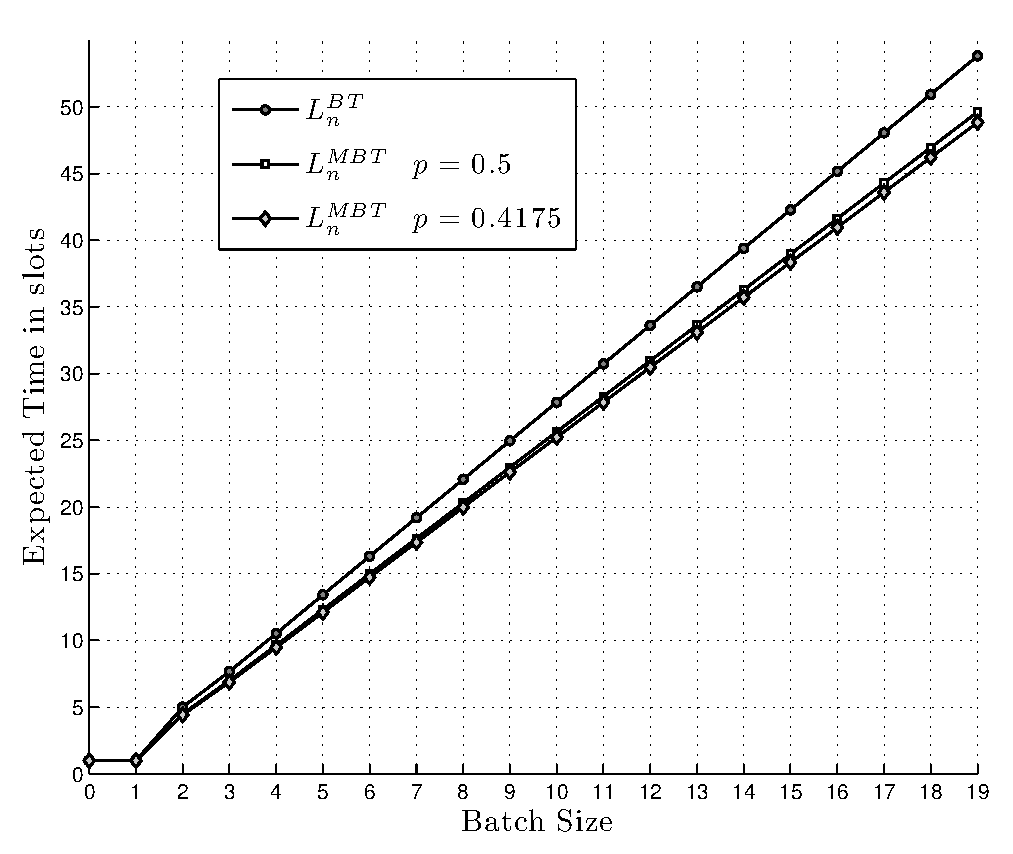
\includegraphics[width=0.7\textwidth]{matlab/BTs/bin-trees-expected-time}
\caption[Expected cost for tree algorithms in \emph{slotted-ALOHA} scenario]{The plot illustrates the expected cost in slots to solve batches of size $n=0,1,\ldots,19$ in a \emph{slotted} Aloha-like scenario using all the basic variants of the tree based algorithms: BT, MBT with sub-optimal $p=0.5$, MBT with optimal $p=0.4175$. All the algorithms show the same behavior: almost linear grow for large $n$. Best performance are provided by MBT with optimal $p$.}
\label{fig:BTs performances}
\end{center}
\end{figure}

Considering the efficiency $\eta_{n}=n/L_{n}^{BT}$ (number of resolved nodes over slots) we have a decreasing series $\eta_{1}=1$, $\eta_{2}=0.40$, $\eta_{3}=0.3913$, \dots, $\eta_{16}=0.3542$ , \dots, $\eta_{31}=0.3505$. It can be shown \cite{capetanakis} that $\eta_{\infty} \approx 0.347$.\\

Since the algorithm is much more efficient in solving small rather than large batches we would prefer to have (ideally)  $n$ batches of size 1 rather than 1 batch of size $n$.\\
Hence, knowing exactly the cardinality $n$ of the initial batch $\mathcal{B}$, we can split the nodes into small groups, of approximately one node each, and resolve them faster. \\This is the idea behind many improvements over the basic BT and it reveals the importance of having an accurate estimate of $n$ to efficiently solve a batch.

\begin{comment}
\begin{figure}
\centering
\begin{tikzpicture}[level/.style={->,thick,level distance = 20mm, sibling distance=40mm/#1}]

\node [circle,draw] (z) {$-,2$}
  {child{node [circle,draw] (a) {0,2} edge from parent
            node[ sloped, above, pos=.6] {$Q_{0}(2)$}}
  child {node [circle,draw] (b) {1,1} edge from parent
            node[ right, pos=.6] {$Q_{1}(2)$}}
  child {node [circle,draw] (c) {2,0}{child [grow=up]{node {} edge from parent [draw=none]}} edge from parent
            node[ sloped, above, pos=.6] {$Q_{2}(2)$}}
};
\end{tikzpicture}
\caption[\emph{BT}: Batch split probabilities]{Transaction probabilities to split a set of 2 elements into two sets with $i$, $j$ elements}
\end{figure}
\end{comment}

\subsubsection{Example}

\begin{figure}[htbp!]
\centering
\ovalbox{
\begin{tikzpicture}[level/.style={thick,level distance = 17mm, sibling distance=80mm/#1}]

\node [circle,draw,label=below:\itshape C,label=above:$\epsilon$] (r){1}{
  	child{node [circle,draw,label=below:\itshape C] {2} {
		child{ node [circle,draw,label=below:$n_{1}$] {3} edge from parent node[ above, pos=.5] {0}
			}
		child{ node [circle,draw, label=below:\itshape C] {4}{		
			child{ node [circle,draw,label=below:$n_{2}$] {5} edge from parent node[ above, pos=.6] {0}}
			child{ node [circle,draw,label=below:$n_{3}$] {6} edge from parent node[ above, pos=.6] {1}}
			} edge from parent node[ above, pos=.5] {1}}
			} edge from parent node[above, pos=.5] {0}
  		}
  	child {node [circle,draw, label=below:\itshape C] {7}{
		child{ node [circle,draw, label=below:\itshape C] {8}{
			child{ node [circle,draw,label=below:\itshape I ] {9} edge from parent node[ above, pos=.6] {0}}
			child{ node [circle,draw,label=below:\itshape C] (s10){10} {
				child{ node [circle,draw,label=below:$n_{4}$] {11} edge from parent node[ above, pos=.6] {0}}
				child{ node [circle,draw,label=below:$n_{5}$] (s12){12} edge from parent node[above, pos=.6]{1} }
			}edge from parent node[ above, pos=.6] {1}}
		} edge from parent node[ above, pos=.5] {0}}
		child{ node [circle,draw,label=below:\itshape I ] {13} edge from parent node[ above, pos=.5] {1}}
		} edge from parentnode[ above, pos=.5] {1}
	}
	
};
\end{tikzpicture}
}
\caption[\emph{BT}: Basic binary tree example]{An istance of BT algorithm for $n=5$ nodes. The number inside each circle identifies the slot number. The label below identifies the event occurring: \textit{I} for \emph{idle}, \textit{C} for \emph{collision}, $n_{i}$ for resolution of node $i$. 0/1 branches is analogous to head/tail.}.
\label{example-bbt}
\end{figure}

In Figure \ref{example-bbt} we provide an example to further investigate the behavior of the algorithm. We notice that the instance starts with a collision in slot 1. Then nodes $n_{1}$, $n_{2}$, $n_{3}$ decide to proceed with a retransmission while $n_{4}$, $n_{5}$ remain idle. In slot 2 we see another collision, after it $n_{1}$ transmits again while $n_{2}$ and $ n_{3}$ to stay quiet. In slot 3 we have the first resolution, $n_{1}$ successfully sends its message and leaves the collision resolution algorithm.\\
We notice that we can know the cardinality of a collision only after it has been fully  resolved. For example we know only after slot 6 that the collision in slot 2 involved 3 nodes.\\

\begin{comment}
\subsubsection{Nodes addresses}

Looking carefully to the tree you can see that each node resolved is characterized by an \emph{address}: the path from the root to node $n_{i}$ gives  a string of bits. For example node $n_{4}$'s address has as prefix 1010. The prefix in this case can be equivalent to the address but, in a more general case, node address can be a longer string. Assuming in fact that node $n_{4}$'s full address is the 8 bit long string 10100010, running the algorithm brings to the discovery of only the first 4 bits since the collision become resolved without requiring further split of the batch and deeper collision tree investigation (collision in level $t$ provokes a split and a deeper investigation in the tree at level $t+1$ and it requires to consider bit $t+1$ of the nodes' addresses).\\
\end{comment}

\subsubsection{Nodes \emph{id} interpretation}
\label{realvalueapproach}
BRAs require each node to have a \emph{unique id} to solve the batch. Usually the nodes \emph{id}s are random generated at each algorithm run and can be used to identify a node inside the algorithm. 
There are multiple ways to generate that the \emph{id}, such as:
\begin{itemize}
\item flipping a coin on demand after each collision (step-by-step \emph{id} generation),
\item generating a `long enough' random binary string  at the beginning of the algorithm.
\end{itemize}
We do not want to enter in the details of these choices since there is no reason to prefer one method to the others but device technical limitations.\\ 
We just want to introduce an interesting interpretation of the \emph{id} that will be used later in algorithms such as EBT (Section \ref{se:EBT}) and Cidon (Section \ref{se:cidon}).\\

In general any infinite length binary string $\mathbf{b_{i}}=(b_{i1}b_{i2}b_{i3}\ldots)$, with $b_{ij} \in \{0,1\}$, can be associated to a real number $r_{i} \in [0,1)$ by a bijective map $r$ defined as follows:

\begin{equation}
r_{i}=r(\mathbf{b_{i}})=\sum_{j=1}^{\infty} \ \frac{b_{ij}}{2^{j}}
\end{equation}
\emph{Each node $n_{i}$ can be associated to a point $r_{i}$ within the real interval [0,1) as well as to the string $\mathbf{b_{i}}$}.\\
For a finite length bit-string $\mathbf{a}=(a_{1}a_{2}\ldots a_{L})$ with length $L=l(\mathbf{a})$ we adapt the definition of $r$ as follows:
\begin{equation}
r(\mathbf{a})=\sum_{j=1}^{L} \ \frac{a_{j}}{2^{j}}
\end{equation}
In this case we have to carry $L$ as auxiliary information to allow the map to remain bijective.\\
Following standard conventions, the empty string $\epsilon$ is prefix of any other string, it has length 0 and $r(\epsilon)=0$.
\begin{comment}
\textcolor{red}{QUESTA OSSERVAZIONE é SOLO FRUTTO DEL MIO SACCO E MI SEMBRAVA INTERESSANTE.\\
An interesting observation is that the distribution of the nodes into the real interval depends upon $p$, the probability  to obtain 0 or 1 tossing a biased coin.
è interessante perchè per il basic binary tree p ottimo è 0.5 per cui si ottiene una distribuzione sperabilmente uniforme dei nodi (o poisson?). Mentre 0.5 non è ottimo per il Modified binary tree: p ottimo 0.4175. quindi la distribuzione migliore per il MBT è una specie di esponenziale discreta e la profondità dell'albero aumenta più ci si avvicina a 1. Questo è quello che mi dice l'intuizione e non ho visto scritto da nessuna parte (magari sul paper orginale del MBT c'è). per cui il MBT non può essere utilizzato banalmente per fare stime tramite una risoluzione parziale di un qualunque sotto intervallo $[0,x)$ con k nodi poichè $n \neq \frac{k}{x} $ (popovski) a meno che non sia nota la distribuzione dei nodi $f(x) $e si normalizzi per $f(x)$ al posto che $x$. 
NOTA: in popovski pg 295  dicono \emph{To summarize, we can say that without any modification, the BT (or the MBT) algorithm offers a way to estimate the unknown conflict multiplicity}. il che è ok ma solo se MBT usa p=0.5
per cui $f(x)=x$. studiare $f(x,p)$?}
\end{comment}

\subsubsection{Tree traversal rules}
The duality in the interpretation of nodes' \emph{id}s (bit-strings or real numbers) reflects on the duality of the tree traversal rules.\\
According to the adopted approach, enabled nodes can be specified by:
\begin{itemize}
\item a finite length string $\mathbf{a}$ which matches the path from  the root to the first node in the sub-tree they belong to. In this case $\mathbf{a}$ is a prefix  of the enabled nodes \emph{id}s.
\item the couple $ \big(r(\mathbf{a}),l(\mathbf{a})\big)$ which enables the sub-interval $r(\mathbf{a})\leq x <r(\mathbf{a})+{\displaystyle{\frac{1}{2^{l(\mathbf{a})}}}}$
\end{itemize}

\begin{comment}
\textcolor{red}{
The inquirer must provide feedback about the event in a slot but tree walking can be either explicit or implicit. It is explicit if, with feedback, the reader provides also the address in the root of the currently enabled sub-tree. Otherwise it is said to be implicit and each node compute autonomously the new enabled sub-tree.}\\
\end{comment}

To complete the overview of the algorithm we now intuitively describe the tree visit. The following description uses the bit-string approach since a binary string can be immediately mapped to a path in the tree starting from the root.
We assume, following the standard approach, to visit the tree in pre-order, giving precedence to left sub-trees, conventionally associated to 0 branches.\\
The visit starts from the root which has address $\epsilon$.\\
Let $\mathbf{a}$ be the current enabled string, then the following rules apply:
\begin{itemize}
\item If $\mathbf{a}=\epsilon$ and last the event is success or idle then the whole conflict has been resolved;
\item If the last event is collision then we visit the left child of the current node ($\mathbf{a}0$);
\item If the last event is success or idle and $\mathbf{a}_{L}=0$ then we visit the right sibling ($\mathbf{a}_{L-1}1$) of the current enabled node;
\item If the last event is success or idle and $\mathbf{a}_{L}=1$ then we look in the path back to the root for the first node whose sibling has not yet been visited. Since we visit the tree in pre-order the next enabled string will be in the form $\mathbf{a}_{k}1$ with $k<L$.
\end{itemize}

A detailed pseudo-code of an algorithm that implements the rules above (and more) can be found in \cite{popovski}. The \emph{Modified Binary Tree} algorithm presented in next section gets a remarkable performance improvement over BT by adding just one new rule.\\

\begin{comment}
Let $b_{1..k}$, with $b_{i} \in \{0,1\}$, $k \geq0$, be the current enabled $k$-bit prefix and \emph{event} $\in \{I,S,C\}$.\\
The possible cases are: \textcolor{red}{qui incasino un po' le cose con una notazione un po' imprecisa}
\begin{enumerate}[i.]
\item \emph{event} is $C$: no matter about $b_{1..k}$, next enabled interval will be $b_{1..k}0$;
\item \emph{event} is not $C$ and $b_{k}=0$: we successfully resolved the left part of the sub-tree, now we will look for right one. Next enabled prefix will be $b_{1..k-1}1$;
\item \emph{event} is not $C$ and $b_{k}=1$: we completed the  resolution of a left sub-tree, now we will look in the way back to the root for the first right sub-tree still unresolved. Let $t$ be $ \arg\underset{i \in 1..k}{\max}|b_{i}=0$ (or $t\gets 0$ if $b_{1..k}$ having 1 or more 1), in other words the position of the right most 0 in the prefix, if any. The new enabled interval will be $b_{t-1}1$. You can see this rule applied after slot 6 and 12 in the example;
\item termination condition is checking $b_{1..k}=\epsilon$.
\end{enumerate}
\end{comment}

\subsection{Modified Binary Tree}
\label{se:MBT}

The \emph{Modified Binary Tree (MBT)} is a simple way to improve the BT algorithm.\\ 
\rev{
To keep the notation simple, we will explain the idea illustrating what happens the first time it is applied. In this case  node $\tau$ is visited in slot $\tau$. This does not holds in general, but explanation would have required to use two different indexed for slots and nodes, and Figure \ref{example-mbt} would have been less immediate to understand.\\}

The observation is that, during the tree traversal, sometimes we know in advance if the next slot will be collided. This happens when, after a collided slot $\tau$, we get an idle slot ($\tau+1$) in the left branch of the binary tree. In this case, visiting the right branch ($\tau+2$), we will certainly get a collision .\\
\rev{In fact, after sensing slot $\tau$ is collided, we know that there are at least 2 nodes in the last visited sub-tree. None of them belongs to the left-branch  of that sub-tree since slot ($\tau+1$) is idle. Consequently they must be in the right branch of the sub-tree, whose enabling will hence result into a collision.
 This collision can be avoided by skipping node ($\tau+2$) and visiting its left-child node in slot ($\tau+2$).\\}

\begin{figure}[htbp!]
\centering
\ovalbox{
\begin{tikzpicture}[scale=1, level/.style={thick,level distance = 17mm, sibling distance=80mm/#1}]

\node [circle,draw,label=below:\itshape C,label=above:$\epsilon$] (r){1}{
  	child{node [circle,draw,label=below:\itshape C] {2} {
		child{ node [circle,draw,label=below:$n_{1}$] {3} edge from parent node[ above, pos=.5] {0}
			}
		child{ node [circle,draw, label=below:\itshape C] {4}{		
			child{ node [circle,draw,label=below:$n_{2}$] {5} edge from parent node[ above, pos=.6] {0}}
			child{ node [circle,draw,label=below:$n_{3}$] {6} edge from parent node[ above, pos=.6] {1}}
			} edge from parent node[ above, pos=.5] {1}}
			} edge from parent node[above, pos=.5] {0}
  		}
  	child {node [circle,draw, label=below:\itshape C] {7}{
		child{ node [circle,draw, label=below:\itshape C] (s8) {8}{
			child{ node [circle,draw,label=below:\itshape I ] (s9){9} edge from parent node[ above, pos=.6] (s89){0}}
			child{ node [circle,draw,blue,label=below:\itshape \textcolor{blue}{C},label=45:\textcolor{blue}{SKIP}] (s10){10} {
				child{ node [circle,draw,label=below:$n_{4}$] (s11){11} edge from parent node[ above, pos=.6] (s1011){0}}
				child{ node [circle,draw,label=below:$n_{5}$] (s12){12} edge from parent node[above, pos=.6]{1} }
			}edge from parent node[ above, pos=.6] {1}}
		} edge from parent node[ above, pos=.5] {0}}
		child{ node [circle,draw,label=below:\itshape I ] {13} edge from parent node[ above, pos=.5] {1}}
		} edge from parent node[ above, pos=.5] {1}
	}	
};
%scale=0.8
%\draw [-latex,blue,thin,dashed] (s9) .. controls ++(46:1.6) and ++(0.5,1.6) .. (s11);
%\draw [-latex,blue,thin,dashed] (s11) to [bend left ](s12);
%scale =1;
\draw [-latex,blue,thin,dashed] (s9) .. controls ++(45:2) and ++(0.5,2) .. (s11);
\draw [-latex,blue,thin,dashed] (s11) to [bend left ](s12);
\end{tikzpicture}
}
\caption[\emph{MBT}: Modified binary tree example]{Same example as in Figure \ref{example-bbt} but using \algname{MBT}: tree structure do not change but node 10 is skipped in the traversal.}
\label{example-mbt}
\end{figure}

Expected time analysis is analogous  to Section \ref{basicbinarytreedescription}. The only difference is that after a collision, if we get an idle slot, we will skip the ``next one'' (saving a slot that would certainly be wasted otherwise). Consequently the expected slot cost is $\left[1 \cdot \bigl(1-Q_{0}(n)\bigr)+ 0\cdot Q_{0}(n)\right]$. Let $L_{n}^{MBT}$ be the expected cost in slots to solve a batch of size $n$ using the MBT algorithm, then\\
\begin{equation}
L_{n}^{MBT} = \bigl(1 - Q_{0}(n)\bigr)+\sum_{i=0}^{n} Q_{i}(n) (L_{i}^{MBT}+L_{n-i}^{MBT}),
\end{equation}
with
\begin{equation*}
L_{0}^{MBT} = L_{1}^{MBT}  = 1.
\end{equation*}
\rev{Intuitively in this case, since a higher probability to stay silent reduces the expected slot cost, optimal transmit probability will be no longer equal to one half.} At the same time, reducing the transmit probability will increase the number of (wasted) idle slots. Thus the new optimal probability $p$ will be somewhere in the interval (0,0.5).\\
It can be shown \cite{massey} that the best result is achieved for $p=0.4175$, for which the efficiency is asymptotically equal to $\eta \approx 0.381$. This is  +10\% higher than basic BT.\\
In general we have 
\begin{equation}
L_{n}^{MBT}\leq C \cdot n +1, \qquad \textrm{where} \qquad C=2.623.
\end{equation}
Using probability $p={\displaystyle\frac{1}{2}}$  results, for large $n$, in about 1.6\% peak performance loss  ($C=2.667$), which is a moderate decrease. It is important to notice that  $p=0.4175$ is very close to the optimal bias for small $n$ as well.\\

\subsection{Clipped Modified Binary Tree}
In this section we will show that, in some cases, partial resolution algorithms can achieve higher efficiency than complete resolution algorithms.\\
The \emph{Clipped Modified Binary Tree (CMBT)} is an adaptation of the \emph{CBT} (see Section \ref{cbt-estimation}) algorithm for complete batch resolution. CBT is like the MBT algorithm but it ends up after two consecutive successful transmissions. Each CBT execution resolves at least two nodes but eventually the last run. Hence, since the multiplicity of the batch to resolve decreases of at least two units after each run, the algorithm terminates for sure.\\

\noindent Collisions tree visit is defined by the following rules: 
\begin{itemize}
\item If the last  run of the CBT does not resolves completely the left sub-tree of the current root, then the next CBT starts from the same root;
\item If the last run of the CBT resolves completely the left sub-tree of the current root, next CBT run is applied to the right child of the current root, that will be considered the new root;
\item While current root left child is \emph{idle}, set the root to the current root right child.
\end{itemize}
Applying the CBT starting each time from the current root makes the algorithm memoryless: its behavior is not affected by previous algorithm runs but the trivial root update. In fact, the root update allows to skip certain collisions and empty slots associated to already resolved sub-sets.\\ 

Efficiency in solving very small batches is CMBT most interesting property. This is a consequence of being memoryless. 
Figures \ref{fig:cmbt-vs-mbt} shows how in the average case, \revv{the CMBT performs a few better than the MBT  for batch sizes smaller than 5. Expected maximum performance improvement is about $5\%$ when batch size is 3.} Nonetheless, for bigger batch sizes, MBT performs better than CMBT and  the gap between the two algorithms gets bigger and bigger as the batch size increases.\\

Consequently, using CMBT is a good idea when the cardinality of the batch to solve is less than or equal to 5 with very high probability. For this reason CMBT is used by the EBT algorithm (following Section \ref{se:EBT}) to speed up the resolution.
  
\begin{figure}[H]
\begin{center}	
    \subfloat[\emph{CMBT vs MBT}: very small batch sizes]{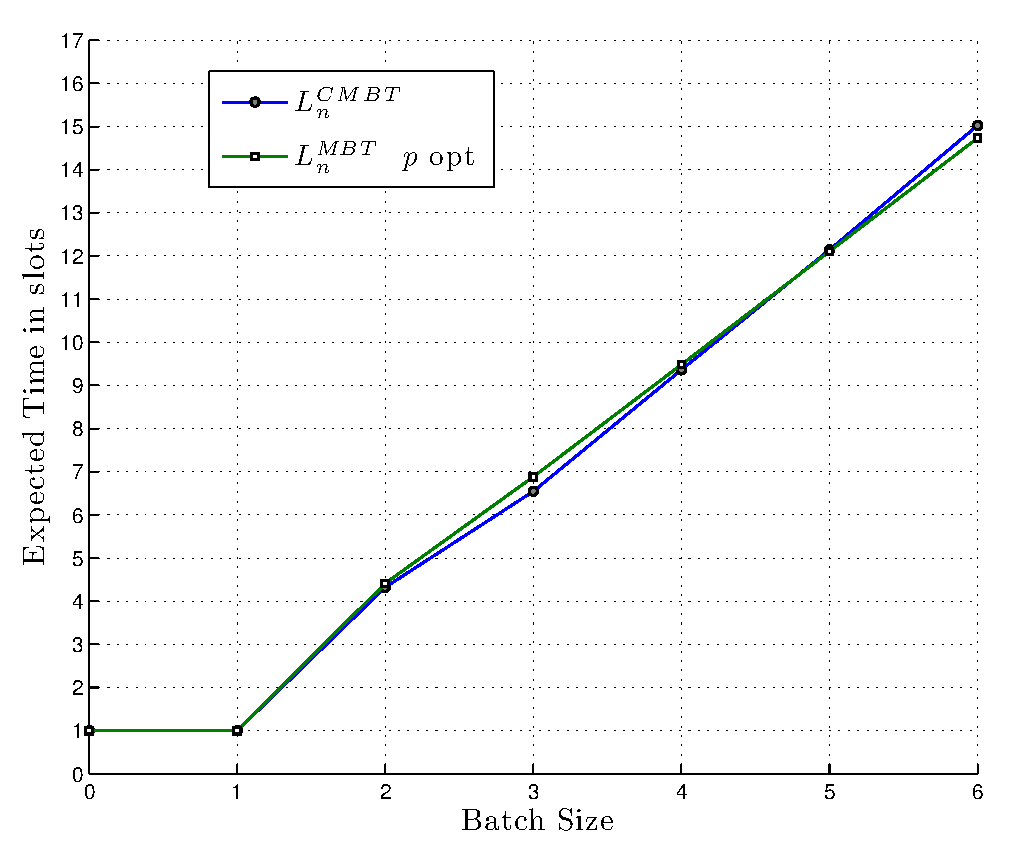
\includegraphics[scale=0.5]{matlab/EBT/CMBT-vs-MBT-small}} 
  \subfloat[\emph{CMBT vs MBT}: larger batch sizes]{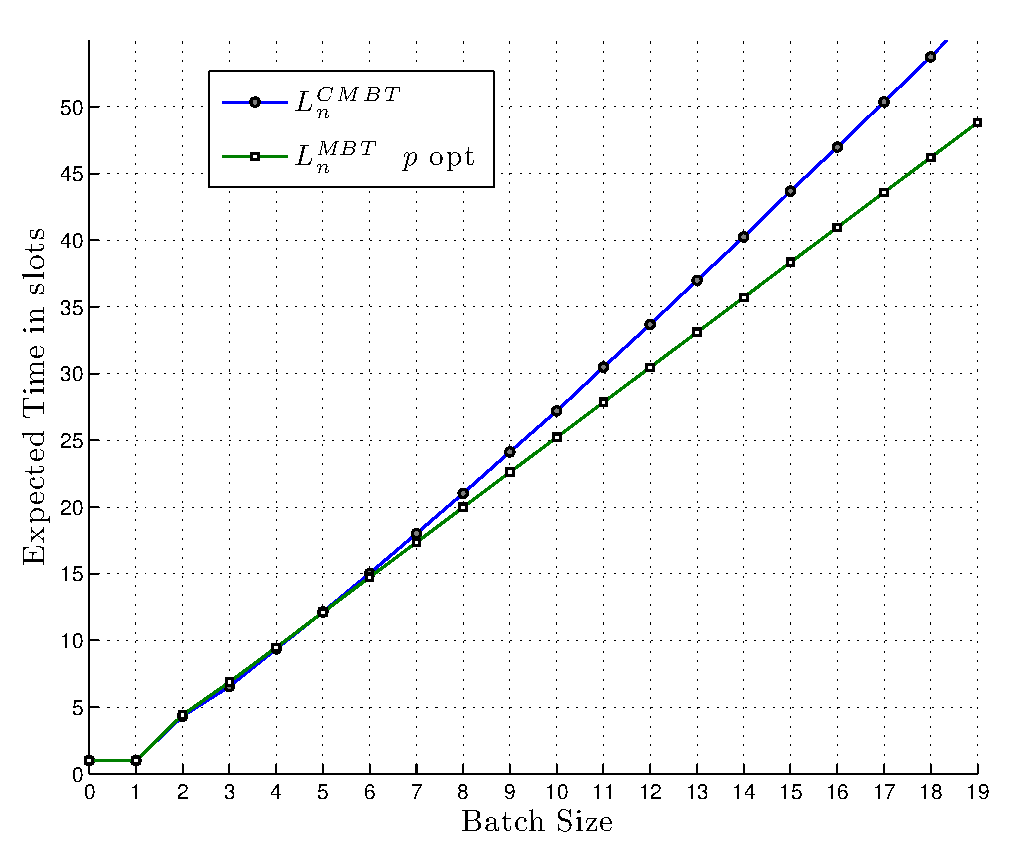
\includegraphics[scale=0.5]{matlab/EBT/CMBT-vs-MBT-large}}
  \end{center}
\caption[\emph{CMBT} vs \emph{MBT}] {Expected resolution time in slots for the \emph{CMBT} and \emph{MBT} algorithms for small batch sizes.} 
\label{fig:cmbt-vs-mbt}   
\end{figure}


\begin{comment}
\begin{figure}[H]
\begin{center}
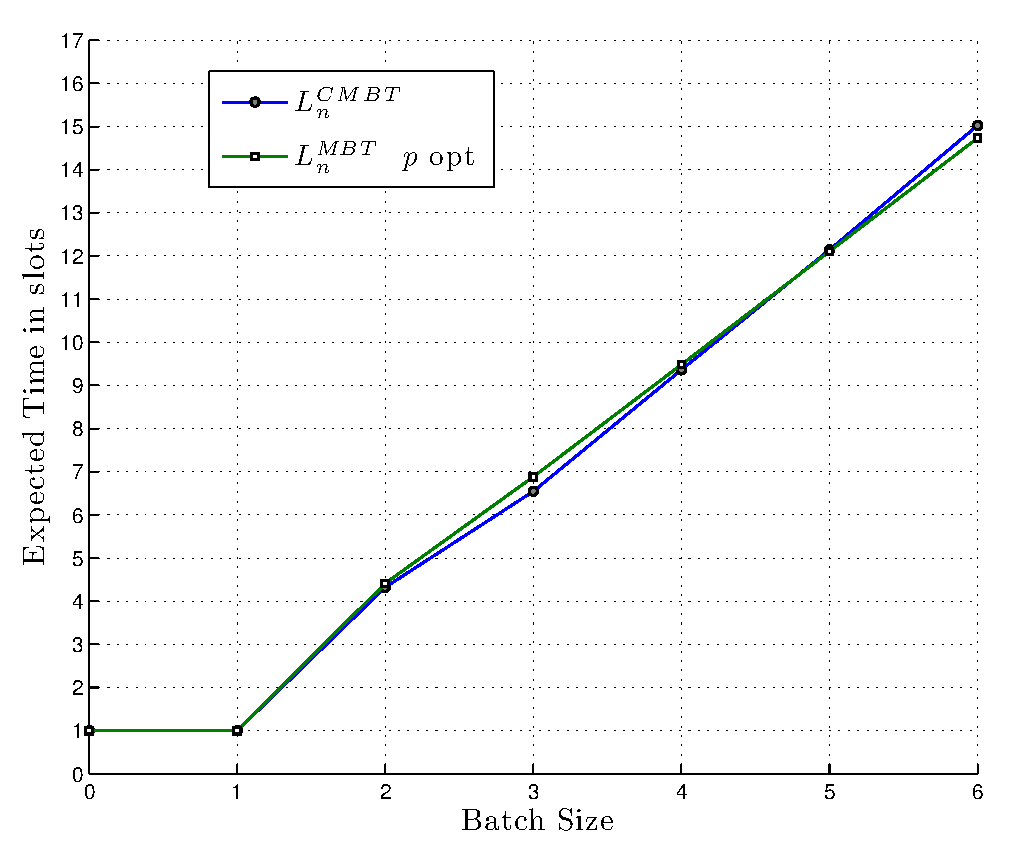
\includegraphics[scale=0.7]{matlab/EBT/CMBT-vs-MBT-small}
\caption{}
\end{center}
\end{figure}

\begin{figure}[H]
\begin{center}
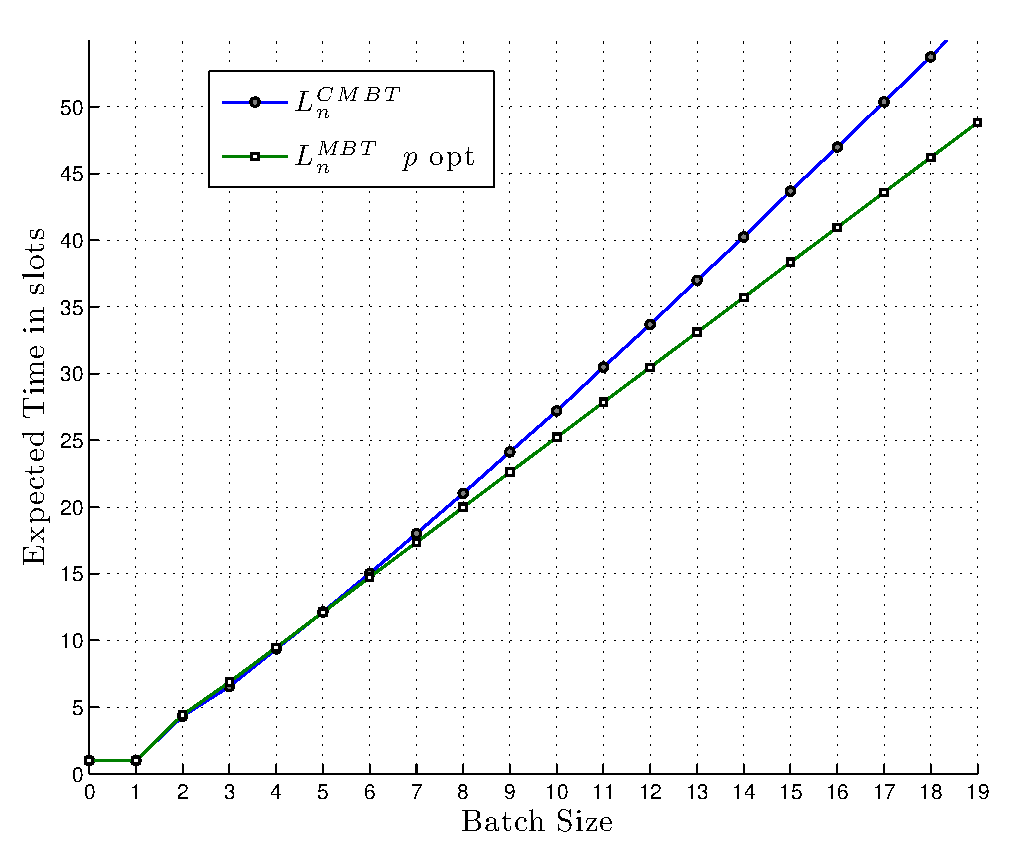
\includegraphics[scale=0.7]{matlab/EBT/CMBT-vs-MBT-large}
\caption{}
\end{center}
\end{figure}
\end{comment}

\subsection{\emph{m} Groups Tree Resolution}
\label{se:mgroups}

More advanced algorithms for batch resolution, such as those presented in \cite{cidon} and \cite{greenberg87}, share a common idea: divide the initial batch into $m$ groups. We will not deal here about the details of the algorithms and the different approaches  they use to choose $m$. Instead we will concentrate on the common part of these algorithms: divide a batch of size $n$ into $m$ groups and apply a BRA to each group.\\
Given $m$ groups, the probability to have exactly $i$ among $n$ nodes in a group is given by
\begin{equation}
P_{m}(i|n)={n \choose i} \left(\frac{1}{m}\right)^{i} \left(1-\frac{1}{m}\right)^{n-i}.
\end{equation}
Let $L_{k}$ be the expected cost to solve a batch of size $k$ with a chosen BRA. Then the expected cost to solve a batch of size $n$ dividing it into $m$ groups is given by
\begin{equation}
\label{eq:BT+m-group-ALOHA}
L'_{n}(\rho)=m \sum_{i=0}^{n}L_{i}P_{m}(i|n),
\end{equation}
where $\rho={\displaystyle\frac{n}{m}}$ is the mean number of nodes in a group.\\
\revv{
Figure \ref{m-groups-MBT-ALOHA} plots $L_{n}'(\rho)$, the average time to solve a batch of size $n$ using group splitting, over $L_{n}$, the average time   without splitting. Results were obtained computing  equation \eqref{eq:BT+m-group-ALOHA} for three different batch sizes varying $\rho$.  We plotted the results for the MBT algorithm with optimal probability $p$ in a slotted ALOHA scenario but considerations hold for any \emph{tree-based BRA}.}


\begin{figure}[H]
\begin{center}
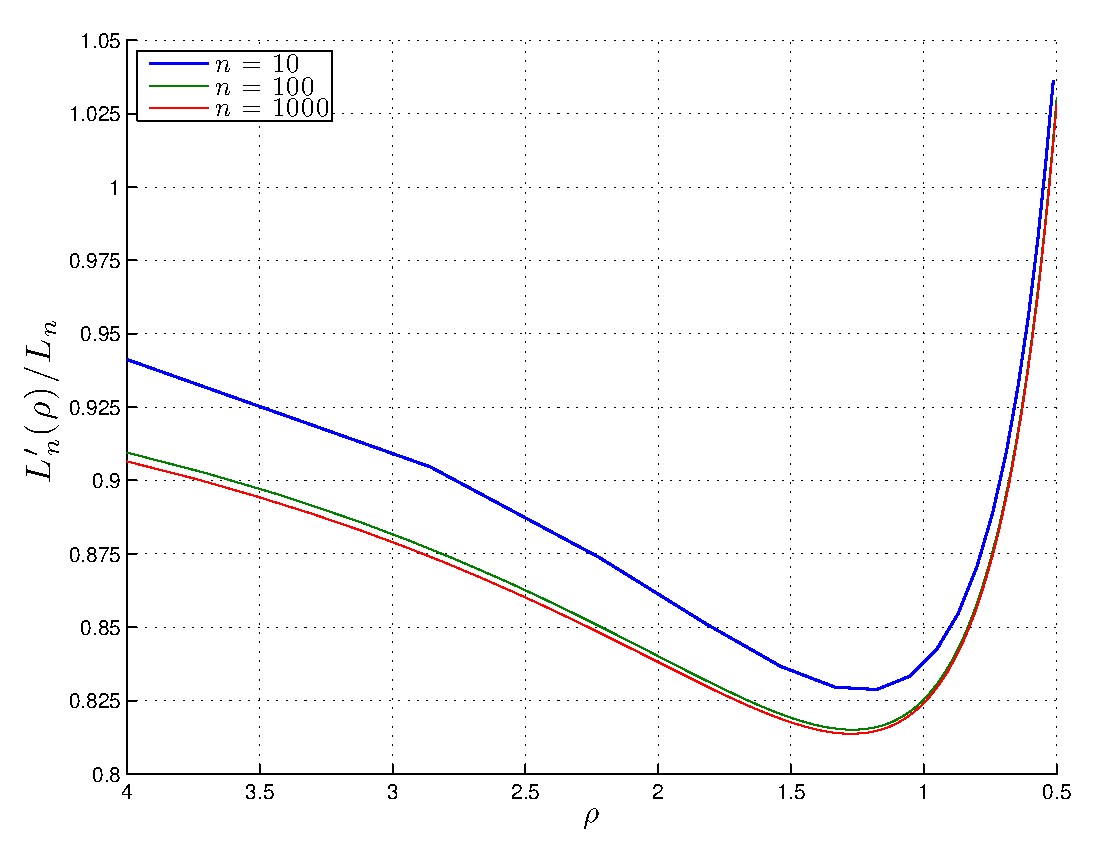
\includegraphics[width=0.7\textwidth]{matlab/BTs/m-groups-MBT-ALOHA}
\caption[$m$ Groups Split: ALOHA scenario]{\emph{$m$ Groups Split: ALOHA scenario}. \revv{Expected performance of group splitting over trivial batch resolution using optimum MBT for different $\rho$. Lower means better}.}
\label{m-groups-MBT-ALOHA}
\end{center}
\end{figure}

\revv{Splitting the batch into groups achieves lower average resolution time than applying the BRA to the original batch for a wide range of $\rho$ \mbox{(when $L_{n}'(\rho)/L_{n}<1$)}.}\\
We note that  $\rho\approx 1.26$ provides the best achievable performance. Furthermore we notice that the knowledge of the batch size is critical: $m$ can be set to the optimal value only knowing exactly the batch size $n$ but often we only have an estimate of $n$. If the estimate is smaller than $n$, performances smoothly degrade but still remain better than the trivial application of the BRA. On the other hand, overestimating $n$ can lead to performance loss when $\rho \approx 0.5$ or smaller.\\

In a CSMA scenario the performances depend also on $\beta$ and on the ratio between the nodes packet size ($S_{n}$) and the supervisor feedback size ($S_{f}$). Figure \ref{m-groups-MBT-CSMA} was obtained considering $\displaystyle\frac{S_{n}}{S_{f}}\approx4$. We notice that in CSMA increasing idle slots probability ($\rho$ small) can lower the expected cost. CSMA is also much more robust to an overestimate of $n$ than \emph{slotted}-ALOHA.

\begin{figure}[H]
\begin{center}
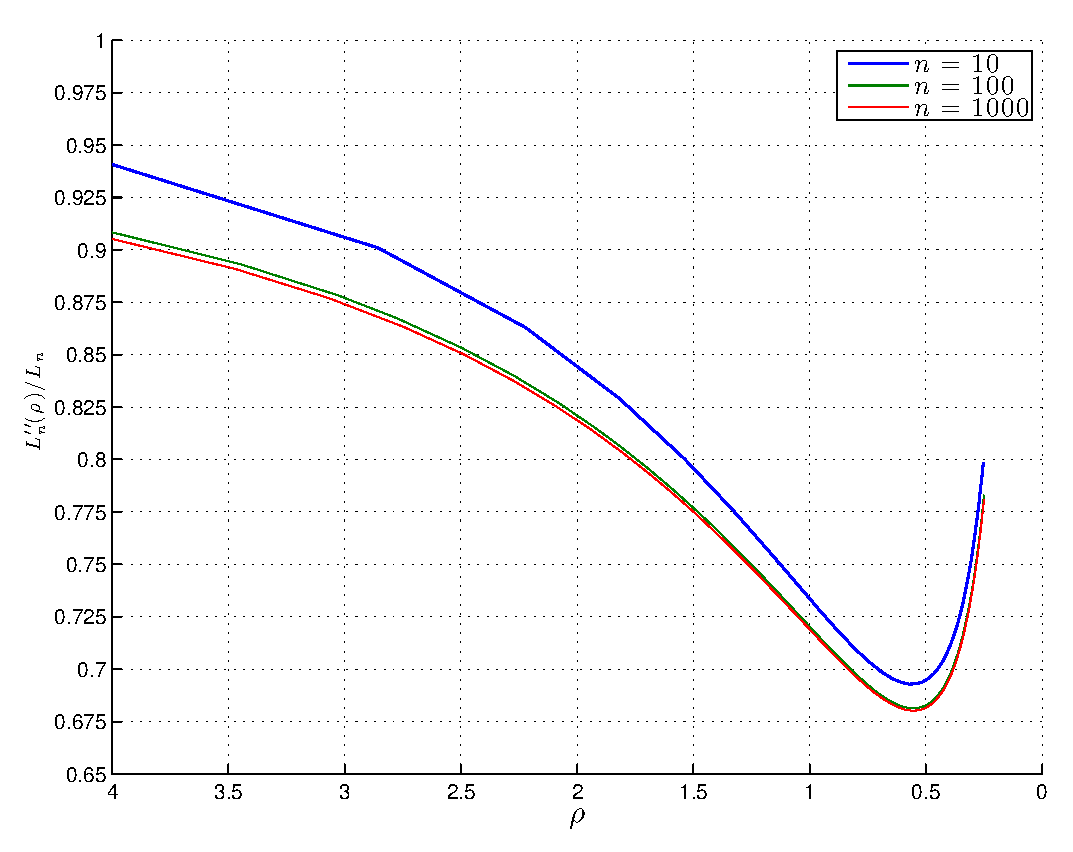
\includegraphics[width=0.7\textwidth]{matlab/BTs/m-groups-MBT-CSMA}
\caption[$m$ Groups Split: CSMA scenario]{\emph{$m$ Groups Split: CSMA scenario}.  \revv{Expected performance of group splitting over trivial batch resolution using optimum MBT for different $\rho$. Lower means better}.}
\label{m-groups-MBT-CSMA}
\end{center}
\end{figure}


\subsection{Estimating Binary Tree}
\label{se:EBT}
\marginpar{NUOVA}
\emph{Estimating Binary Tree} (EBT) has been recently proposed in \cite{popovski}. It does not work on parameters optimization but tries to use simple heuristics to skip tree nodes that will result in collisions with high probability.\\
Given a batch of size $n$, the keys to understand EBT are the following:
\begin{itemize}
\item in the luckiest scenario, running BT results in a balanced binary tree where all the leaves are at the same level,
\item consequently it seems to be a good idea to assume that nodes at levels in the tree less than $\lfloor \log_{2}n\rfloor$ will likely result in collided slots.
\end{itemize}

EBT tries to skip inner nodes of the tree by visiting only nodes at levels equal or deeper than $\lfloor \log_{2}n\rfloor$. Since $n$ is not \emph{a priori} known, a dynamic estimating technique is adopted. To effectively use this estimate tecnique each node must be able to generate values from the standard uniform distribution on the interval [0,1) and to use that value as its unique \emph{id}.\\
 Assume that there are $k$ nodes whose \emph{id}s are in the sub-interval [0,$\pc$) and that they have been previously resolved: all and only the nodes with \emph{id} less than $\pc$ successfully transmitted their messages.  Let $\hat{n}$ express the estimate of $n$. When $\pc$ is greater than 0, setting $\hat{n}$ to $\displaystyle\frac{k}{\pc}$ provides a good estimate of $n$ that becomes more and more accurate as the algorithm goes on. EBT uses $\hat{n}$ (as soon as it is available) to choose the right level in the tree to analyze.\\
 
 The most straightforward  interpretation of the EBT algorithm can be:

\begin{algorithm}
\caption{\algname{Estimating Binary Tree}}
\begin{algorithmic}
\STATE  Run the CBT algorithm
\WHILE{batch is not resolved}
\STATE  Update the estimate $\hat{n}$
\STATE Start a new CMBT at the next node from level $\lfloor\log_{2}\hat{n}\rfloor$
\ENDWHILE
\end{algorithmic}
\end{algorithm}

Here we gave only a short insight of the algorithm and the estimate technique. In particular this estimate technique is a dynamic adaptation of that described later in Section \ref{se:cidon} and originally proposed in \cite{cidon}.\\

\begin{comment}
\subsection{EBT combined with optimum MBT (DA BUTTARE)}

In this section we describe an improvement over EBT we developed.\\
EBT assumes the nodes to be uniformly distributed in the interval [0,1): this means that their \emph{id} is generated flipping a fair coin. This is a necessary condition for the collision tree to be balanced (the expected height of each leaf is the same) and allows to estimate the level in the tree to analyze using $\lfloor\log_{2}\hat{n}\rfloor$.\\ We remember also that the optimal probability $p$ that provides the best performance  for the MBT is $p=0.4175$. Nevertheless, when $p$ is optimum, the recursive splitting of the original set into 2 subsets, whose expected size is $np$ and $n(1-p)$, returns an unbalanced collision tree.\\ 

\noindent The ideas are the following: 
\begin{itemize}
\item Initially nodes \emph{id}s are uniformly distributed in the tree,
\item Changing a part of a node \emph{id} is allowed if this doesn't affects the already visited conflicting sets,
\item After a collision takes place in a node at level $\hat{N}=\lfloor\log_{2}\hat{n}\rfloor$, the devices involved in the collision  can be redistributed in the collided domain.
\end{itemize}

Let each node $n_{i}$ to be identified by a $L$-length binary string $\mathbf{b_{i}}=(b_{i1}b_{i2}\ldots b_{iL})$. Applying the MBT we resolve a sub-batch or, otherwise, get a collision. In case of collision each node involved updates its \emph{id} as follows: $\mathbf{b_{i}}=(b_{i1}b_{i2}\ldots b_{i\hat{N}}c_{i1}\ldots c_{i(L-\hat{N})})$ where $c_{ik}=0$ with probability $p=0.4175$ and $c_{ik}=1$ with probability $1-p$.\\  

\noindent This modified version of EBT can be briefly described as follows:
 \begin{enumerate}
\item Run the CBT algorithm;
\item Repeat until the end of the process the following steps:
\begin{enumerate}[a)]
\item Update the estimate $\hat{n}$;
\item Start a new MBT at the next node at level $\lfloor\log_{2}\hat{n}\rfloor$ and perform only the first transmission;
\item If the transmission results in a collision, colliding nodes regenerate their \emph{id};
\item Continue  with the current MBT.
\end{enumerate}
\end{enumerate}

\begin{figure}[htb]
\begin{center}
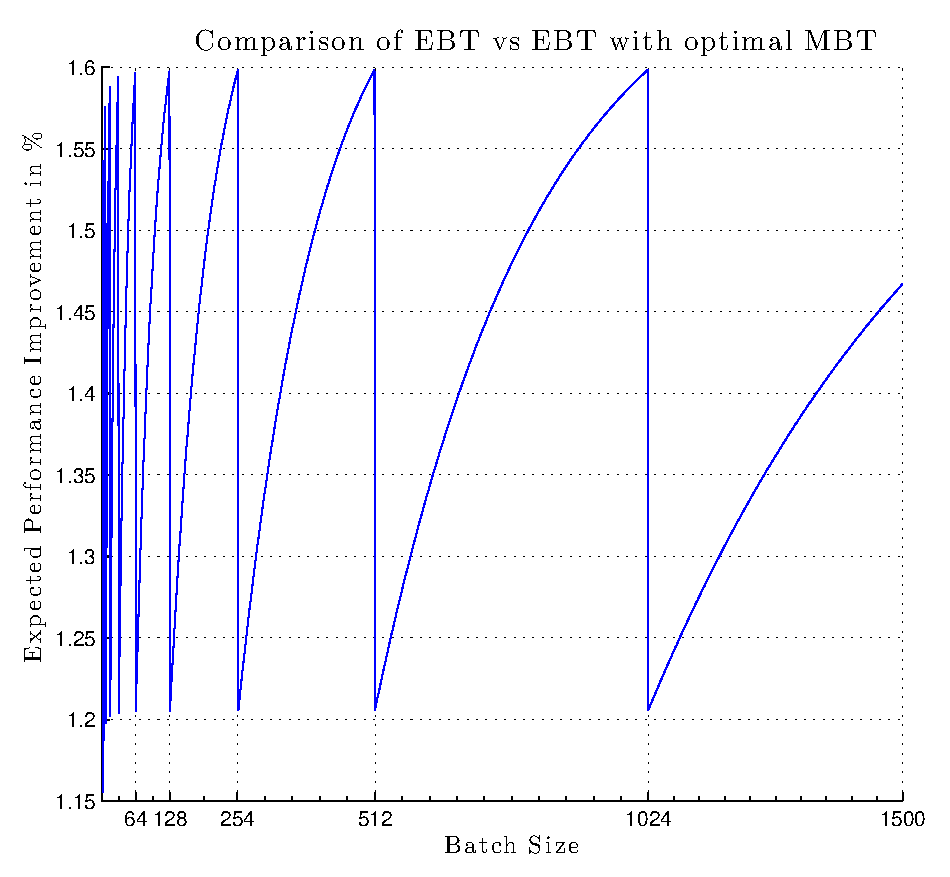
\includegraphics[scale=0.7]{matlab/BTs/EBT-EBT_MBT-Comparison}
\caption[\emph{EBT} vs \emph{EBT with optimal MBT} Performance Comparison]{EBT with optimal MBT provides a minimum expected performance improvement over EBT of 1.2\% and 1.42\% in mean.}
\label{EBTvsEBTopt}
\end{center}
\end{figure}

Figure \ref{EBTvsEBTopt} shows the expected improvement in percentage between  the EBT and the modified EBT algorithm in terms of expected cost ratio. Performance gain results oscillatory with mean 1.42.\\

The \emph{EBT using optimum MBT Algorithm}, proposed in this work, is the average case best \emph{tree-based algorithm with implicit estimate} known so far.

\end{comment}

\section{Others}
In this section we will shortly describe non \emph{tree-based} algorithms for batch resolution.
\subsection{IERC}
The \emph{Interval Estimation Conflict Resolution (IERC)} \cite{popovski} is an adaptation of the FCFS \cite{gallager} algorithm for Poisson's arrivals of packets to the batch resolution.\\
FCFS is the fastest known algorithm to solve Poisson's arrivals and it achieves efficiency $\eta=0.4871$.
It assumes \emph{a priori} knowledge of the arrival rate $\lambda$ of the packets and works by splitting the time in epochs of length $\tau$.\\
Now we briefly describe FCFS algorithm. and then we will show how it can be translated to the batch resolution problem.\\ 

At any time $k$, let $T (k)$ be the start time of the current enabled allocation interval. Packets generated in the enabled window $(T(k),T(k)+\tau]$ are allowed to be transmitted.
When an \emph{idle} or \emph{successful} event occurs enabled time window gets incremented (shifted towards current time) by $\tau$. On the other hand, if a \emph{collision} takes place, a \emph{Clipped Binary Tree} (see Section \ref{cbt-estimation}) algorithm is started. Given that CBT resolves the sub-interval $(T(k),T(k)+\alpha(k)]$, then next FCFS enabled window at time $k'$ will be $(T(k'),T(k')+\min(\tau,k'-T(k'))]$ where $T(k')=T(k)+\alpha(k)$.\\

It can be shown \cite{gallager} that setting  $\tau={\displaystyle \frac{1.26}{\lambda}}$ leads to the maximum efficiency. This means that, on average, there are 1.26 nodes in an allocation interval of length $\tau$.\\
The batch resolution problem can be adapted to be solved with an FCFS-like strategy in the following way:
\begin{itemize}
\item nodes \emph{tokens} can be interpreted as arrival times;
\item nodes must be splitted into $m={\displaystyle \frac{n}{1.26}}$ groups, so that in each group we expect to have 1.26 nodes;
\item apply FCFS to solve the problem.
\end{itemize}
\revv{Following  these ideas, IERC achieves the same efficiency $\eta=0.4871$ of FCFS for Poisson's arrivals in solving the \emph{Batch Resolution Problem}: it is the asymptotically fastest know algorithm allowed by our scenario model. }

\subsection{Window Based Approaches}

Another possible approach to the batch resolution is to consider a \emph{framed}-ALOHA scenario.\\
In \emph{framed}-ALOHA, a frame (or \emph{window}) is a sequence of consecutive slots.  When a node in the collision batch decides to transmit, it uniformly picks one and only one slot in the window and transmits in that slot.\\
In windows based scenarios, usually we can work on the optimization of two parameters: $m$, the length of the window in slots, and $p$, the probability that a node transmits in the current window.
Innovative approaches to the problem uses hybrid transmission scheme working by cycles that tries to optimize operational parameters after each transmission windows.


\chapter{Batch Size Estimate Techniques}
\label{ch:Batch Size Estimate Techniques}
Here we present some noteworthy techniques for batch size estimate that can be found in the literature.
If a technique was not already identified by a name or associated to an acronym, we used the name of one the authors as reference.\\

In general, we assume to have no \emph{a priori} statistical knowledge about the conflict multiplicity. Estimation techniques are thus required to provide accurate estimates for the general zero-knowledge scenario.\\
\section{Clipped Binary Tree}
\label{cbt-estimation}
A simple way to obtain an estimate of the batch size is to solve a certain number of nodes and then infer the batch size according to the time taken to solve these nodes. This can be done, for example, by using deterministic algorithms such as the \emph{Clipped Binary Tree (CBT) Algorithm}.\\
CBT is a partial resolution algorithm since only a fraction of the packets of the batch are successfully transmitted.
The algorithm is identical to the MBT, with $\displaystyle p=\frac{1}{2}$ since we require nodes to be uniformly distributed in the interval [0,1), except that it stops (the tree is clipped) whenever two consecutive successful transmissions follow a conflict.\\
When the algorithm stops, after $i$ collisions, we know than the last two resolved nodes belong to the same level $i$ of the tree (root is assumed to be at level 0). Therefore, an estimate of the initial batch size is given by:
\begin{equation}
\hat{n}\gets2^{i}
\end{equation}
\begin{comment}
The idea is interesting but the fact of considering recursively subsets of subsets of the initial batch brings to disastrous performance: as reported in \cite{greenberg87}, second and all higher moments of this estimate are infinite.\\
So this simple method is not good to obtain an estimate. 
\end{comment}

\begin{figure}[H]
\centering
\ovalbox{
\begin{tikzpicture}[level/.style={thick,level distance = 17mm, sibling distance=80mm/#1}]

\node [circle,draw,label=below:\itshape C,label=above:$\epsilon$] (r){1}{
  	child{node [circle,draw,label=below:\itshape C] {2} {
		child{ node [circle,draw,label=below:$n_{1}$] {3} edge from parent node[ above, pos=.5] {0}
			}
		child{ node [circle,draw, label=below:\itshape C] {4}{		
			child{ node [circle,draw,label=below:$n_{2}$] {5} edge from parent node[ above, pos=.6] {0}}
			child{ node [circle,draw,label=below:$n_{3}$] {6} edge from parent node[ above, pos=.6] {1}}
			} edge from parent node[ above, pos=.5] {1}}
			} edge from parent node[above, pos=.5] {0}
  		}
	child {node {} {child {node {} edge from parent[draw=none]} child {node {} edge from parent[draw=none]}}edge from parent[draw=none]}
};
\end{tikzpicture}
}
\caption[\emph{CBT}: Example]{ Same example as in Figure \ref{example-bbt} but resolution using CBT ends up after two consecutive successful transmissions.}
\end{figure}

Experimental results show that the variance of this estimate is extremely high and the resulting accuracy is rather poor. This is due to the fact that the batch we use for the estimate becomes, at each level, smaller and smaller. Using this algorithm we do not have knowledge of a sufficiently large number of intervals but we limit to analyze only a few leafs.
The resulting estimate, even for huge sizes, depends only on very few (3-5) outer nodes (those at the most left in the tree). Consequently estimate is quite inacurate.\\
From the tables  \ref{CBT-table-1} reported in Appendix you can notice that the distribution probability decreases rather slowly.
\section{Cidon}
\label{se:cidon}
In \cite{cidon} Cidon and Sidi proposed a complete resolution algorithm based on two phases:
 
\begin{enumerate}
\item Estimate the initial batch size using a partial deterministic resolution scheme. 
\item Perform an optimized complete deterministic resolution based on the results of phase 1. 
\end{enumerate}

Phase 1 consists in resolving a small part of the initial batch, counting the number of successful transmissions.
A node takes part either to the estimate phase or to the following resolution phase, not both.
The probability $\pc$, which is an algorithm input parameter, determines this choice.
We called it $\pc$ to underlined that this initial choice reflects the expected accuracy of the resulting estimate, as it will be discussed in more detail later on.\\

As usual we consider a batch $\mathcal{B}$ of unknown size $n$.
At the beginning of the algorithm each node chooses to transmit with probability $\pc$. Thus the $n$ nodes are partitioned into two sets, $\mathcal{E}$ and $\mathcal{D}$, where $\mathcal{E}$ consists of those that transmitted and $\mathcal{D}$ the rest. Clearly, $|\mathcal{E}|+|\mathcal{D}|=n$. If the resulting slot is empty or contains a successful transmission, we conclude that $|\mathcal{E}|=0$  or $|\mathcal{E}|=1$, respectively. When a conflict occurs ( $|\mathcal{E}|\geq2$), nodes in $\mathcal{E}$ use a complete BRA to resolve the conflict among them. Let $j$ be the number of resolved nodes at the end of phase 1, i.e. $|\mathcal{E}|=j$. Then the estimate $\hat{n}$ is given by 

\begin{equation}
\hat{n} \gets \frac{j}{\pc}.
\end{equation}
When the nodes are uniformly distributed in the real interval [0,1), $\displaystyle \frac{j}{\pc}$  identifies also the expected nodes density in the interval [0, 1) and the nodes in $\mathcal{E}$ are those whose \emph{id} can be mapped to a value belonging to the sub-interval [0, $\pc$).\\
Figure \ref{cidon-nodes-id} illustrates the concept with a simple example.
\begin{figure}[H]
    \centering
    \ovalbox{
    \begin{tikzpicture}
    \draw [thick, [-)] (0,0) node[label=below:0] {}-- (10,0) node[label=below:1] {};
    
    \foreach \x / \y in{1/$n_{1}$,2/$n_{2}$,3.5/$n_{3}$,4/$n_{4}$,5.5/$n_{5}$,7.6/$n_{6}$,9.2/$n_{7}$}
    \draw[->] (\x,1) node [label=above:\y]{} -- (\x,0.3);
    
    % 
    \draw[->] (3,-1) node [label=below:$<\pc\leq$]{} -- (3,-0.3);
    \draw[snake=crosses, very thick] (3,0) node [label=above:0.3] {}-- (3.2,0);
    
    \end{tikzpicture}
    }
    \caption[\emph{Cidon}: Initial split]{In this example $\pc=0.3$. At the beginning of the algorithm each node generates its own \emph{id} from the standard uniform distribution in the interval [0,1). Nodes whose \emph{id} is less than $\pc$ belongs to $\mathcal{E}$. Nodes whose \emph{id} is greater or equal to $\pc$ belongs to $\mathcal{D}$. Estimate of the batch returns $\lceil 2/0.3\rceil=7$ which, in this case, is the exact size of the batch.}
    \label{cidon-nodes-id}
\end{figure}

After the first phase,  nodes in $\mathcal{E}$ are resolved, whereas those in $\mathcal{D}$ have still to be counted. An estimate $\hat{k}$ of $|\mathcal{D}|$ can be obtained as
\begin{equation}
\hat{k} \gets  \frac{j}{\pc}(1-\pc).
\end{equation}
This estimate is used as starting point for the second phase of the Cidon algorithm, whose  high level peudo-code is presented in Algorithm \ref{alg-cidon}.
 
 \begin{algorithm}[h!]
\begin{algorithmic}[1]
	\REQUIRE $\mathcal{B}$ batch with $|\mathcal{B}|=n$
	\REQUIRE $\pc$, fraction of the whole batch to solve
	\STATE \COMMENT{Phase 1}
	\STATE each node flips a coin getting 0 with probability $\pc$, 1 otherwise
	\STATE $\mathcal{E} \,\gets$ \{ nodes that flipped 0\}
	\STATE $\mathcal{D} \gets$ \{ nodes that flipped 1\}
	\STATE \algname{Complete collision resolution ($\mathcal{E}$) }
	\STATE  $\hat{k} \gets |\mathcal{E}|/\pc$
	\STATE \COMMENT{Phase 2}
	\STATE \algname{Optimized complete collision resolution ($\mathcal{D}$,$\hat{k}$, $\pc$) }
	\end{algorithmic}
\caption{\algname{Cidon($\mathcal{B}$, $\pc$)}}
\label{alg-cidon}
\end{algorithm}
\noindent\algname{Complete collision resolution ($\mathcal{E}$) } identifies any procedure able to resolve all the nodes in $\mathcal{E}$ allowing them to successfully transmit their messages.\\ \algname{Optimized complete collision resolution ($\mathcal{D}$,$\hat{k}$, $\pc$) } identifies an optimized way to resolve the batch $\mathcal{D}$ that takes into account the expected multiplicity of $\mathcal{D}$.\\
 
 The original paper proposes to use an \emph{$m$ groups split} (Section \ref{se:mgroups}) approach to resolve $\mathcal{D}$, where 
 \begin{equation}
m = \max(1, \lceil\alpha \hat{k}-\beta\rceil),
\end{equation}
and each group is resolved by applying the MBT algorithm.\\
The parameter $\alpha$ determines the number of groups, and therefore the efficiency of the resolution process, when $n$ is large, while $\beta$  reduces the number of groups when $n$ is small in order to reduce the risk of empty groups. 
 
 $\alpha=0.786$ determines $\rho\approx 1.27$ which is the \emph{unique} \revv{optimum  nodes per group density}. $\beta$ and $\pc$ depend on operational requirements: in \cite{cidon} it is showed that setting $\beta=8$ and  $\pc=0.1$ is a good compromise to get efficient resolution for a wide range of batch sizes.\\  
 
The average  cost of the estimate phase \revv{(phase 1)} depends on the BRA used but in general, for tree-based BRAs,  can be considered $O(\pc n)$.

\begin{comment}
\subsection{Estimate accuracy}
%%%%%%%%%%%%%%%%%%%%%%%%%%%%%%%%%%%%
\label{cidon-estimate-accuracy}

In the original paper \cite{cidon} there is no detailed analysis of the behavior of the estimate algorithm, but it is only shown the following fact: as $n$ grows the estimator becomes more accurate.\\
    
Let $J$ be an integer random variable that expresses the number of nodes in $\mathcal{E}$. Given a batch of size $n$, $J$ is binomially distributed with parameter $\pc$. Therefore, we have the following:

\begin{equation}
	P(J=j|n)={n \choose j}\pc^{j}(1-\pc)^{n-j},
           \label{cidon-J}
\end{equation}

\begin{equation}
E[J|n]=n\pc ,
\label{cidon-e-estimate}
\end{equation}

\begin{equation}
\textrm{var}(J|n)=n\pc(1-\pc).
\end{equation}


By applying Chebychev's Inequality \eqref{eq:cheby},  we have for any $\epsilon>0$
 
 \begin{equation}
P\Bigl( \left| J-n\pc\right| \geq \epsilon n \,|\, n \Bigr) \leq \frac{\pc(1-\pc)}{\epsilon^{2}n}.
\label{eq:cidon-cheby}
 \end{equation}
 
 Let $\hat{N}={\displaystyle \frac{J}{\pc}}$ be a real-valued random variable that expresses our estimate of $n$. Then from the aforementioned equations \eqref{cidon-J} - \eqref{eq:cidon-cheby}, it follows that:

\begin{equation}
P\left(\hat{N}=\hat{n}|n\right)={n \choose j}\pc^{j}(1-\pc)^{n-j} \quad \textrm{with} \quad \hat{n}=j/\pc, \quad 0\leq j\leq n,
\end{equation}

\begin{equation}
E[\hat{N}|n]=n,
\end{equation}
and, finally,
 \begin{equation}
P\left( \left| \frac{\hat{N}}{n}-1\right| \geq \epsilon  \,\big|\, n \right) \leq \frac{1-\pc}{\epsilon^{2}n\pc}.
 \end{equation}
which shows that in this estimation method we can trade off the accuracy with the consumption of resources in terms of time or messages.
%%%%%%%%%%%%%%%%%%%%%%%%%%%%%%%%%%%%%%
\end{comment}
\section{Greenberg}


\emph{Basic Greenberg algorithm} searches for \emph{a power of 2} that is close to $n$ with high probability:
\begin{equation}
\hat{n}\geq 2^{i} \approx n
\end{equation}
Let each of the $n$ conflicting stations either or not transmit in accordance with the outcome of a biased binary coin. The coin is biased to turn up 0 (transmit) with probability  $2^{-i}$ and 1 (do not transmit) with complementary probability $1-2^{-i}$. Since the expected number of transmitters in the slot is $2^{-i}n$, a conflict supports the hypothesis that $n\geq2^{i}$.\\
Using this test repeatedly with $i=1, 2, 3, \ldots$, leads to the Greenberg \emph{base 2 estimation algorithm}.\\
Each of the conflicting stations executes Algorithm (\ref{alg-greenberg}), resulting in a series of collisions whose length determines $\hat{n}$.
The probability that at most one node transmits in a slot, monotonically grows with the slot number and approaches 1 very rapidly as $i$ increases beyond $\log_{2}n$. Consequently, we expect that the collision series stops at slot $i$ that is close to $\log_{2}n$.\\

\begin{algorithm}[H]
\begin{algorithmic}
\STATE \COMMENT Each node performs these operations
\STATE $i\gets 0$
\REPEAT
	\STATE $i\gets i+1$
	\STATE choose to transmit with probability $p=2^{-i}$
\UNTIL {no collision occurs}
\STATE $\hat{n} \gets 2^{i}$
\end{algorithmic}
\caption{\algname{Basic Greenberg ($\mathcal{B}$)}}
\label{alg-greenberg}
\end{algorithm}

The idea behind Algorithm \ref{alg-greenberg} appears to be quite simple: as the algorithm goes on, the initial unknown batch (of size $n$) is progressively sliced into smaller pieces. Only the nodes virtually inside the enabled slice are allowed to transmit. Slices get thinner and thinner until at most one node is contained in a slice. Figure \ref{fig:greeberg-split} illustrates the idea with an example:
visually, nodes can be thought to be uniformly distributed on a circumference. Using Greenberg algorithm we will analyze at each slot a smaller sector (in this case the half of the previous one) of the circle and discover when a sector contains at most 1 node. Note that no overlapping sectors are drawn to maintain the image simple. However, in general, enabled nodes get redistributed at each transmission test performed by the algorithm.\\
\begin{figure}[htb!]
    \centering
    \begin{tikzpicture}[scale=0.8]  
        \draw (0, 0) circle (3.8cm);
        \foreach \x in {3.5,13.5,...,360}
        \draw[snake=crosses] (\x:3.7) --(\x:3.8);
       \draw[-,ultra thin,dashed] (180:6) to[] (0:6); 
       \draw[-,ultra thin,dashed] (0,0) to[] (-90:6);
       \draw[-,ultra thin,dashed] (0,0) to[] (-135:6);
       \draw[-,ultra thin,dashed] (0,0) to[] (-157.5:6);
       \draw[-,ultra thin,dashed] (0,0) to[] (-168.75:6); 
       \draw[-,ultra thin,dashed] (0,0) to[] (-174.375:6);  
        %arco rosso
        \foreach \x/\text in {1.6,1.7,...,2.5}
        \draw [-,thin,red!50] (0:\x) arc(0:-90:\x);
        %arco  blue
        \foreach \x/\text in {2.6,2.7,...,3.5}
        \draw [-,thin,blue!50] (0:\x) arc(0:180:\x); 
        %arco verde
        \foreach \x/\text in {.6,.7,...,1.5}
        \draw [-,thin,green!80] (-90:\x) arc(-90:-135:\x);

        \draw [<->,ultra thin,blue] (5:5) arc(5:175:5);
        \draw [<->,ultra thin,red] (-5:5.3) arc(-5:-85:5.3);
        \draw [<->,ultra thin,green] (-95:5.6) arc(-95:-130:5.6);
        
        \path[text width=3pt]
        (90:6)      node[above right] {$\pi$}  (95:2)      node[below] {$n/2$}
        (-45:6)      node[below right] {$\pi/2$} (-50:2.7)      node[right] {$n/4$}
        (-112.5:6)      node[below left] {$\pi/4$} (-118:2)      node[below left] {$n/8$};
    \end{tikzpicture}
    \caption{\emph{Basic Greenberg}: batch split idea}
    \label{fig:greeberg-split}
\end{figure}

Expected running time is $O(log_{2}\,n)$. In particular, since in the \emph{slotted}-ALOHA model, feedback is supposed to be transmitted at the end of each transmission slot, the expected running time in slots can be expressed as $\approx 1+\log_{2}n$.\\

An important note is that the algorithm always involves all the nodes in the batch: at each slot, each node decides whatever or not transmit. Each choice is independent of the past.
This is of great importance and allows $\hat{n}$ to have bounded statistical moments: it can be shown that, for large $n$, it holds:
\begin{equation}
E[\hat{n}] \approx n\phi,
\end{equation}
\begin{equation}
E[\hat{n}^{2}] \approx n\Phi,
\end{equation}
where
\begin{equation}
\phi= \frac{1}{\log2} \int_{0}^{\infty} \! e^{-x}(1+x) \prod_{k=1}^{\infty}\bigl(1-e^{-2^{k}x}(1+2^{k}x)\bigr)x^{-2} \, dx = 0.91422
\end{equation}

\begin{equation}
\Phi= \frac{1}{\log2} \int_{0}^{\infty} \! e^{-x}(1+x) \prod_{k=1}^{\infty}\bigl(1-e^{-2^{k}x}(1+2^{k}x)\bigr)x^{-3} \, dx =1.23278
\end{equation}

\noindent $\phi$ and $\Phi$ are obtained in \cite{greenberg87} using advanced mathematical analysis supported by Mellin integral transform\footnote{In this work we only report the final results. Please, refer to the original paper for details.}.
In general $\phi$ and $\Phi$ depend on the size of the problem. Table \ref{table:phi-Phi} shows the behavior of the expected estimate (and, therefore of $\phi$) as a  function of $n$. We note that the ratio $E[\hat{n}|n]/n$ monotonically decreases and gets stable at $0.9142$. This shows that this estimate technique provides biased results.\\

\begin{table}[htb]
\caption{\emph{Basic Greenberg}: Expected estimate and bias}
\begin{center}
\begin{tabular}{rD{.}{.}{5.2}D{.}{.}{1.4}}
\toprule
 n & \multicolumn{1}{r}{$E[\hat{n}|n]$} & \multicolumn{1}{c}{$E[\hat{n}|n]/n$} \\ \midrule
1 &     2.00 &   2.0000 \\ 
2 &     2.56 &   1.2822 \\ 
4 &     4.21 &   1.0533 \\ 
8 &     7.89 &   0.9863 \\ 
16 &  15.20 &   0.9498 \\ 
32 &    29.82 &   0.9320 \\ 
64 &    59.08 &   0.9231 \\ 
128 &   117.59 &   0.9186 \\ 
256 &   234.60 &   0.9164 \\ 
512 &   468.64 &   0.9153 \\ 
1024 &   936.71 &   0.9148 \\ 
2048 &  1872.86 &   0.9145 \\ 
4096 &  3745.14 &   0.9143 \\ 
8192 &  7489.72 &   0.9143 \\ 
16384 & 14978.86 &   0.9142 \\ 
32768 & 29957.16 &   0.9142 \\ 
65536 & 59913.74 &   0.9142 \\\bottomrule
\end{tabular}
\end{center}
\label{table:phi-Phi}
\end{table}
The fact that, for large $n$, $E[\hat{n}] \approx n\phi$ suggests a way for correcting the estimate bias as $\hat{n}_{+} = {\displaystyle\frac{\hat{n}}{\phi}}$. Due to the contribution of periodic functions, $\hat{n}_{+}$ is not an asymptotically unbiased estimate of $n$, in the sense that  $E[\hat{n}_{+}]/n$ does not tend to 1 as $n$ gets large. Fortunately, the amplitude of the periodic functions turns out to be less than $2 \cdot10^{-5}$, so this bias is negligible for all practical purposes.\\


Interestingly, a simple variant of the estimation algorithm shows really poor performance. Consider the algorithm in which each station involved in the initial collision transmits to the channel with probability $1/2$. If this causes another collision, then those that just transmitted, transmit again with probability $1/2$. The others drop out. This process continues until there are no collisions. Let $2^{i}$ be the estimate of the conflict multiplicity, where $i$ is the slot  at which there is no collision. It can be shown \cite{greenberg87} that the second and all higher moments of this estimate are infinite.

\subsection{Base \emph{b} variant}

Using basic Algorithm \ref{alg-greenberg}, the expected value of $\hat{n}_{+}$ is likely different from $n$ by a factor 2. In the original work, a small generalization of the base 2 algorithm is proposed to overcome this limitation, by simply using a base $b$ instead of 2, with $1<b\leq2$.\\
\begin{algorithm}[H]
\begin{algorithmic}
\STATE $i\gets 0$
\REPEAT
	\STATE $i\gets i+1$
	\STATE transmit with probability $b^{-i}$
\UNTIL {no collision occurs}
\STATE $\hat{n}(b) \gets 2^{i}$
\STATE $\hat{n}_{+}(b) \gets \hat{n}(b)/\phi(b)$
\end{algorithmic}
\caption{\algname{base \emph{b} Greenberg ($\mathcal{B}$)}}
\label{alg-greenberg-base-b}
\end{algorithm}

In Algorithm \ref{alg-greenberg-base-b}, the term $\phi(b)$ corrects the bias of the estimator. Table \ref{table:greenberg-b-phi} shows how $\phi$ and the expected cost in slots vary for different $b$. Expected cost ($\lesssim \log_{b}n$) is expressed as a multiplicative factor for the basic Greenberg algorithm cost ($\lesssim \log_{2}n$). We can notice that smaller $b$ results in smaller $\phi(b)$. This means that $b$ deeply biases the estimate: if $b^{'} < b^{''}$ then $E[\hat{n}(b^{'})] < E[\hat{n}(b^{''})]$. This follows form the fact that, decreasing $b$, the stop probability ``shift'' towards ``early slots'' associated to lower estimates.   

%nota della tabella, assicurarsi che sia nella stessa pagina

\begin{table}[H]
\caption{\emph{Base $b$ Greenberg}: Bias and expected cost summary}
\label{table:greenberg-b-phi}
\begin{center}
%\begin{threeparttable}
\begin{tabular}{lccl}
$b$ & $\phi(b)$ &\,\,\,& Expected cost in slots-1\\
\toprule
2          & $\approx 0.9142$ && $\lesssim 1 \qquad\,\,\, \times \log_{2} n$\\
1.1       & $\approx 0.3484$ && $ \lesssim 7.27$\\
1.01     & $\approx 0.1960$ && $ \lesssim 69.66$\\
1.001   & $\approx 0.1348$ && $ \lesssim 693.49$\\
1.0001 & $\approx 0.1027$ && $ \lesssim 6931.81$\\
\bottomrule
\end{tabular}
\begin{comment}\tnote{a}\end{comment} 
%\begin{tablenotes}
%\item [a] {\footnotesize \smaller Code used to compute $\phi(b)$ is provided in Appendix \ref{sec:greenberg-moments}}
%\end{tablenotes}
%\end{threeparttable}
\end{center}
\end{table}
\noindent In\cite{greenberg87}, it is shown that, \emph{for all n greater than some constant $n_{0}(b)$, it holds}
	\begin{equation} 
		\left |\frac{E[\hat{n}_{+}(b)]}{n}-1 \right | < \epsilon(b) ,
	  \end{equation}

\begin{equation}
		\frac{\sigma\bigl(\hat{n}_{+}(b)\bigr)}{n}< \epsilon(b) ,
	\end{equation}
\noindent where $\epsilon(b) \to 0$ as $b \to 1$.\\
 In other words when $b \to 1$ and $n$ is large the estimate becomes unbiased and its variance goes to zero. However, our experimental results showed that the performance of base $b$ estimator is not ideal in practical scenarios.  




\section{Window Based}

Window based approaches use a \emph{framed}-ALOHA transmission scheme, where the reader provides feedback to the nodes after each frame. \emph{Framed}-ALOHA is characterized by the frame length $L$, whose choice is critical for the performance of the resolution process as well as the estimation phase. \begin{comment}In fact, in \emph{framed}-ALOHA there is no clear distinction between resolving the nodes and estimating  their number since the estimate can be performed only by knowing the outcome of the last enabled window.\end{comment}\\
Setting $L$ large compared to the batch size increases the probability to solve all the nodes in the current window but, on the other hand, it leads to a waste of slots and consequently sub-optimal running time.  At the same time, a large value of $L$ allows for a very accurate estimate of the batch size.\\
Setting $L$ small increases the probability of collided slots. Since the number of nodes involved in a collision is unknown, collisions provide poor information about the batch multiplicity. The more collisions we have, the less accurate the estimate.\\

An interesting approach to the problem is presented in \cite{lucent}. When the scenario allows to use a \emph{probabilistic-framed-ALOHA}\footnote{\emph{Probabilistic-framed-ALOHA} is an extension of the \emph{framed-ALOHA} model where a node takes part to the current contention window with probabily $p$ or waits for the next one with probability $1-p$. Nodes that decide to transmit behave like in the standard \emph{framed-ALOHA}.} scheme we can act on the parameter $p$, i.e. the probability for a node to take part in the current transmission window. Small $p$ value allows to keep $L$ small too and hence, when $n$ is large, provides an accurate estimate of the whole batch considering only a sub-set of it. This results in shorter estimate time.\\

Since when $p=1$ \emph{probabilistic-framed-ALOHA} reduces to simple \emph{framed-ALOHA} and it is reasonable to start any estimate algorithm with $p=1$, we will show a possible approach to the problem in a \emph{framed-ALOHA} scenario. \\

Let $n$ be the batch size and $L$ the window length. The number of nodes $k$ out of $n$ that choose the same slot is binomially distributed with parameters $B(n,1/L)$. Then, the probability to get an \emph{idle}, \emph{successful} or \emph{collision} slot is respectively given by:
\begin{equation}
p_{0}(n)=\left(1-\frac{1}{L}\right)^{n},
\end{equation}

\begin{equation}
p_{1}(n)=\frac{n}{L}\left(1-\frac{1}{L}\right)^{n-1},
\end{equation}

\begin{equation}
p_{2+}(n)=1-p_{0}(n)-p_{1}(n).
\end{equation}

Considering the whole window, the outcome  consists in a tuple $(i,s,c)$, denoting the number of idle, success, and collision slots, which satisfies $i+s+c=L$.
Hence, the probability of ($i$,$s$,$c$) is given by:
\begin{equation}
P(i,s,c)= \frac{L!}{i!\,s!\,c!} \ p_{0}(n)^{i} \ p_{1}(n)^{s}\ p_{2+}(n)^{c} = \frac{L!}{i!\,s!\,c!} \  \fw(i,s,c,n).
\label{eq:Pisc}
\end{equation}
We note that \eqref{eq:Pisc}, does not take into account the fact that a node is allowed to transmit only once in a window:  equation \eqref{eq:Pisc} is only an approximation of the distribution of the nodes in the slots when both $n$ and $L$ are large. A Poisson distribution of parameter $\lambda=n\frac{1}{L}$ would model better the scenario but \eqref{eq:Pisc} allows simpler numerical computation.\\
Once we have tried to resolve the batch using a window approach we know how many idle, successful or collided slots there were.\\ Then we  find the estimate $\hat{n}$ as the batch size that  maximizes the probability to see the tuple $(i,s,c)$ in a $L$ length window:
\begin{equation}
\hat{n}=\argmax_{\displaystyle n} \fw(i,s,c,n),
\end{equation}
where we discarded the factorial terms because they not contribute to identify the maximum since $L$, $i$, $s$, $c$ are fixed. Furthermore, since $L$, $i$, $s$, $c$ are fixed, $\fw(i,s,c,n)$ becomes a one-variable function which results well behaved in $n$, being initially monotonically increasing and then monotonically decreasing. Therefore $\fw(i,s,c,n)$ has only one maximum.

By setting 
\begin{equation}
\fw'(i,s,c,n)=0,
\label{eq:dummy-eq}
\end{equation}
and numerically solving \eqref{eq:dummy-eq} we can obtain the batch size that maximizes our function. In general the solution will not be integer-valued and a rounding operation is necessary to achieve a real world batch estimate.\\
\begin{table}[H]
\centering
\caption[\emph{Window Based Estimate}: Possible estimates when $L=10$]{Estimate given $(i,c,s)$ when $L=i+c+s =10$.}
\label{tb:window-estimate}
\resizebox{0.6\textwidth}{!}{
\begin{tabular}{|c|c|c|c|c|c|c|c|c|c|c|}
\hline
\backslashbox{$c$}{$s$}&0&1&2&3&4&5&6&7&8&9 \\\hline
1 & 3 & 3 & 4 & 5 & 6 & \multicolumn{1}{r|}{7} & \multicolumn{1}{r|}{8} & \multicolumn{1}{r|}{9} & \multicolumn{1}{r|}{10} &11 \\ \hline
2 & 5 & 6 & 7 & 8 & 8 & \multicolumn{1}{r|}{10} & \multicolumn{1}{r|}{11} & \multicolumn{1}{r|}{12} & \multicolumn{1}{r|}{13} & - \\ \hline
3 & 7 & 8 & 9 & 10 & 11 & \multicolumn{1}{r|}{12} & \multicolumn{1}{r|}{13} & \multicolumn{1}{r|}{14} & - & - \\ \hline
4 & 10 & 11 & 12 & 13 & 14 & \multicolumn{1}{r|}{15} & \multicolumn{1}{r|}{16} & - & - & - \\ \hline
5 & 12 & 14 & 15 & 16 & 17 & \multicolumn{1}{r|}{19} & - & - & - & - \\ \hline
6 & 16 & 17 & 19 & 20 & 22 & - & - & - & - & - \\ \hline
7 & 20 & 22 & 23 & 25 & \multicolumn{1}{l|}{-} & - & - & - & - & - \\ \hline
8 & 26 & 28 & 30 & \multicolumn{1}{l|}{-} & \multicolumn{1}{l|}{-} & - & - & - & - & - \\ \hline
9 & 35 & 38 & \multicolumn{1}{l|}{-} & \multicolumn{1}{l|}{-} & \multicolumn{1}{l|}{-} & - & - & - & - & - \\ \hline
10 & \multicolumn{1}{l|}{$\infty$} & \multicolumn{1}{l|}{-} & \multicolumn{1}{l|}{-} & \multicolumn{1}{l|}{-} & \multicolumn{1}{l|}{-} & - & - & - & - & -\\\hline
\end{tabular}
}
\end{table}

Table \ref{tb:window-estimate} shows the estimate provided by the explained technique when $L=10$. Cells, identified by $(c,s)$, where $c+s>10$ cannot be associated to any estimate since their events are impossible. The case $c=0$ is trivial since the estimate is exact and is given by the number of successful transmission.\\
We note also that when we see only collisions, the estimator is not able to provide a finite estimate. The event $c=10$ in the table is in fact associated to $\hat{n}=\infty$. In general, when $c=L$ we have that \eqref{eq:Pisc} reduces to:

\begin{equation}
P(0,0,L)=\ p_{2+}(n)^{L} = \left[1-\left(1-\frac{1}{L}\right)^{n}-\frac{n}{L}\left(1-\frac{1}{L}\right)^{n-1}\right]^{L},
\end{equation}

\noindent which is maximized ($P(0,0,L)=1$) by $n=\infty$ for any $L$. Hence we would not to have only collisions since they do not provide any information about the cardinality of the batch.\\ A larger  window has to be used to get a finite estimate but its optimal length remains unknown.

\chapter{Estimate Performance Analysis}
\label{ch:Performance Analysis}

In this Chapter, we present a performance analysis of some of the already mentioned noteworthy  \emph{batch size estimation  (BSE) algorithms}. The overview will obviously consider different batch sizes, algorithm parameters, time required and accuracy of the estimate. We want to support reader in choosing the best estimate technique suitable for its needs. \\
First we will provide a detailed analytical analysis of  \emph{Cidon} algorithm and then, supported by numerical computation, we will derive its features in term of time and accuracy.\\  
We will then discuss the behavior of \emph{Greenberg} with its pros and cons and try to overcome its limitations by introducing a modification of the original algorithm to achieve better estimate. \emph{Enhanced Greenberg Algorithm (EGA)} is the middle-step in the development of our proposed estimate algorithm: it improves the estimate in terms of ``choosing the best power of 2'', maintaining the same target estimates allowed by basic Greenberg.  
Then, we will describe and analyze the \emph{Generalized Enhanced Greenberg Algorithm (GEGA)}, which combines Greenberg with a further test and performs a \emph{maximum likelihood estimation} to determine the ``best'' estimate. Finally, the comparison between \emph{GEGA} and \emph{Cidon} will lead to the conclusions.
\section{Cidon BSE}
The original paper \cite{cidon} describes the estimate technique but does not characterize it in details. The interest is focused on other aspects and, therefore, no detailed analysis of the behavior of the estimate algorithm is presented: it is only mentioned that as $n$ grows the estimator becomes more accurate. Hence, in this section we will provide a complete analysis of the estimate algorithm.\\
    
Following from Section \ref{se:cidon}, let $j$ denote the number of nodes in $\mathcal{E}$ and $\pc$ be the expected fraction of nodes to be resolved in Cidon algorithm  Phase 1. Parameter $\pc$ can be considered fixed \emph{a priori} since it is an input of the algorithm and, therefore, given a batch of size $n$, $j$ is a binomially distributed random variable with parameters $n$ and $\pc$. Hence, we have the following:
\begin{equation}
E[j|n,\pc]=n\pc ,
\label{cidon-e-estimate}
\end{equation}
\begin{equation}
\textrm{var}(j|n,\pc)=n\pc(1-\pc).
\end{equation}


By applying Chebychev's Inequality \eqref{eq:cheby},  we have for any $\epsilon>0$
 
 \begin{equation}
P\Bigl( \left| j-n\pc\right| \geq \epsilon n \,|\, n, \pc\Bigr) \leq \frac{\pc(1-\pc)}{\epsilon^{2}n}.
\label{eq:cidon-cheby}
 \end{equation}
 
We remember that the Cidon estimate is given by $\hat{n}={\displaystyle \frac{j}{\pc}}$. Then, from the aforementioned equations \eqref{cidon-e-estimate}-\eqref{eq:cidon-cheby}, it follows that:

\begin{equation}
E[\hat{n}|n,\pc]=\frac{1}{\pc}E\left[j|n,\pc\right]=n, \qquad \forall \,\pc
\end{equation}
and
 \begin{equation}
P\left( \left| \frac{\hat{n}}{n}-1\right| \geq \epsilon  \,\big|\, n,\pc \right) \leq \frac{1-\pc}{\epsilon^{2}n\pc}.
 \end{equation}
which shows that using this estimation method we can trade off the accuracy with the consumption of resources in terms of time or messages. Furthermore, Cidon estimate is unbiased independently of $\pc$, which influences  the variance of the estimator. In fact, we have 
\begin{equation}
\textrm{var}(\hat{n}|n)  =  \frac{n}{\pc}-n
\end{equation}
which reveals that as the number of resolved terminals (and therefore $\pc$) increases the estimate $\hat{n}$ becomes more accurate.
%%%%%%%%%%%%%%%%%%%%%
\begin{comment}
\begin{equation}
\begin{split}
\textrm{var}(\hat{n}|n) & =E[\hat{n}^{2}|n]- E[\hat{n}|n]^{2}\\
& = \frac{1}{\pc^{2}}E[j^{2}|n] - n^{2}\\
& = \frac{n\pc(1-\pc)+n^{2}\pc^{2}}{\pc^{2}}- n^{2}\\
& =  \frac{n}{\pc}-n.
\end{split}
\end{equation}
\end{comment}
%%%%%%%%%%%%%%%%%%%%
\begin{figure}[htbp]
\begin{center}
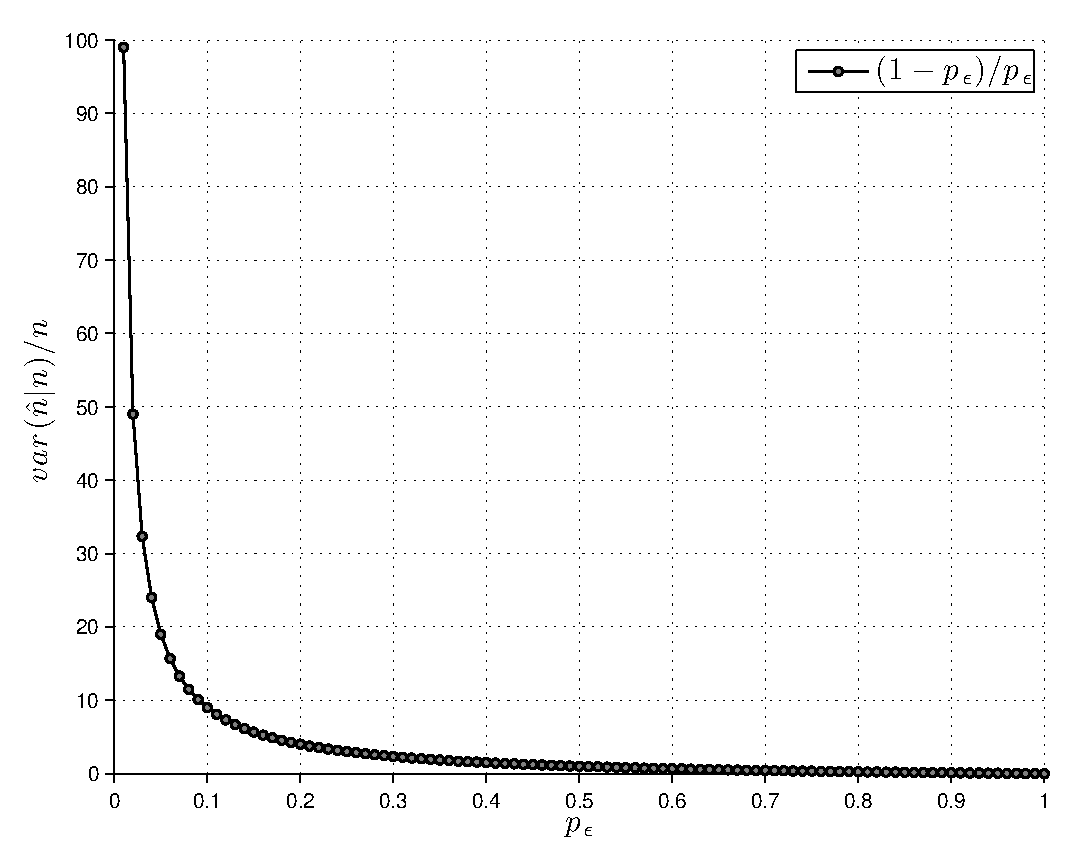
\includegraphics[width=0.7\textwidth]{matlab/Cidon/cidon-variance-p}
%\epsfile{file=matlab/Cidon/cidon-variance-p.eps,scale=0.8}
\caption[\emph{Cidon}: Normalized variance]{\emph{Cidon}:  estimate normalized variance as function of $\pc$.}
\label{fig:cidon-normalized-variance}
\end{center}
\end{figure}

\subsection{Performance}
Figure \ref{fig:cidon-normalized-variance} shows that the variance is strict monotonically decreasing in $\pc$. Furthermore, you can notice that, for $\pc$ smaller than 0.1, a small increment in $\pc$ produces a large decrease in the normalized variance which reflects in a large estimate accuracy improvement. Hence, considering the tread-off between estimate overhead and resolution efficiency, solving up to $\frac{1}{10}$ of the initial batch in the estimate phase is a good practical choice.\\

However, it is difficult to establish in what measure an estimate can be considered accurate. The idea we adopt is to require the estimate to be ``near'' the real batch size with very high probability. 
Given the real batch size $n$, let the \emph{error coefficient} $k \geq1$ identify an interval surrounding $n$ in the following way: 
\begin{equation}
\frac{n}{k}\leq\hat{n}\leq kn
\label{cidon-accuracy-constrains}
\end{equation}
We can study the algorithm behavior by considering as index for the estimate accuracy
\begin{equation}
\theta_{k}=P\left(\frac{n}{k}\leq\hat{n}\leq kn\right)
\label{eq:zanella-bound}
\end{equation}
Let $\theta$ be the minimum allowed value for $\theta_{k}$: in other words $\theta$ is the probability we require for constrains \eqref{cidon-accuracy-constrains} to be satisfied.\\
If we set $\theta=0.99$, we can find the minimum $\pc$, ensuring the estimate to be within interval \eqref{cidon-accuracy-constrains}, by solving the following problem.\\
\begin{equation}
\begin{split}
P\left(\frac{n}{k}\leq \hat{n} \leq kn \big| k,n\right)=& P\left(\frac{n}{k}\leq j/\pc \leq kn \big| k,n,\pc\right)\\
=&P\left(\frac{n\pc}{k}\leq j \leq kn\pc \big| k,n,\pc\right)
\end{split}
\label{cidon-accuracy-bounds}
\end{equation}
Since $j$ assumes positive integer values, we introduce rounding operations. In particular, rounding effect is non neglectible when $n\leq 200$.  \\
\begin{equation}
f(k,n,\pc) = P\left(\left\lceil \frac{n\pc}{k}\right\rceil\leq j \leq \left\lfloor kn\pc\right\rfloor \big| k,n,\pc\right)\geq \theta
\end{equation}
Fixed $k$, $n$ and $\theta$, $\pc$ can be found by numerically solving the following equation:
\begin{equation}
f(k,n,\pc) = \theta
\end{equation}

\begin{figure}[htbp]
\begin{center}
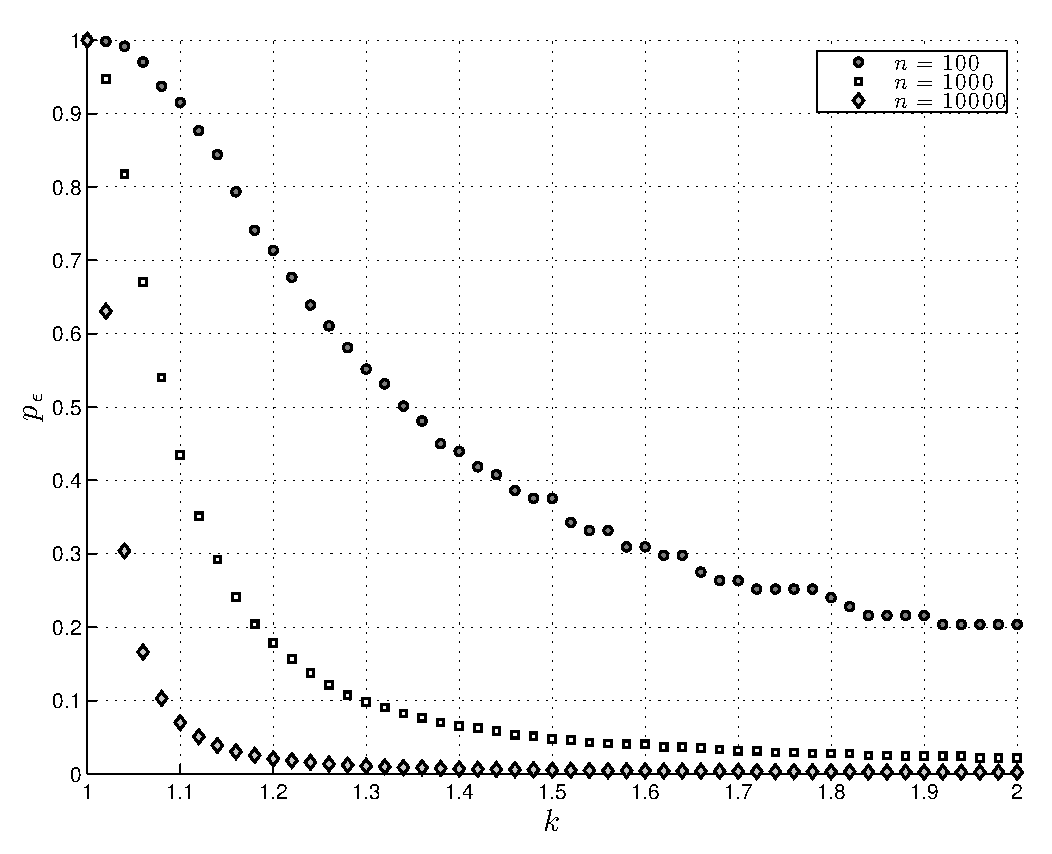
\includegraphics[width=0.7\textwidth]{matlab/Cidon/cidon-k-p-minimum}
\caption[\emph{Cidon}: Minimum $\pc$ required for error coefficient $k$]{\emph{Cidon}: Minimum $\pc$ as function of $k$ when $\theta=0.99$.}
\label{cidon-k-p-minimum}
\end{center}
\end{figure}

Figure \ref{cidon-k-p-minimum} plots the minimum fraction $\pc$ of the batch to be resolved as function of $k$ when $\theta=0.99$. As you could expect, once the batch size is fixed, the minimum $\pc$ is  monotonically decreasing in $k$. In the same manner, when $k$ is fixed, the minimum fraction of the batch to resolve to achieve the desired accuracy is lower for larger batch sizes. In Figure \ref{cidon-k-L-minimum} we report the expected time (in slots) required by \emph{Cidon} to achieve the desired accuracy in the estimate.  We notice that initially, when $k$ is larger than 1.5, the time required to achieve a given accuracy is very similar for each considered batch size. For tighter accuracies the time required depends largely on the size of the problem.\\ Furthermore, the time required by the largest considered batch size to achieve a given accuracy provides an upper bound for smaller batch sizes: in the same amount of time smaller batch sizes are expected to achieve higher accuracy.\\

\begin{figure}[htb!]
\begin{center}
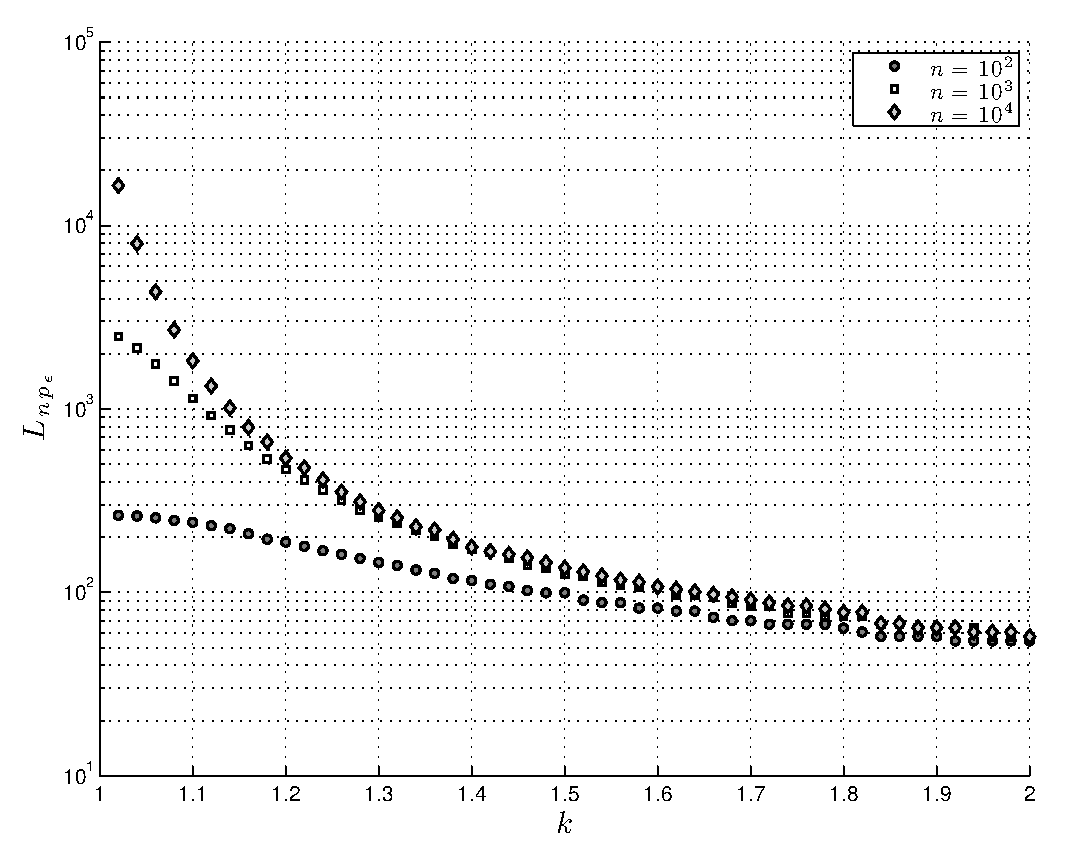
\includegraphics[width=0.7\textwidth]{matlab/Cidon/cidon-k-L-minimum}
\caption[\emph{Cidon}: Expected time as function of the error coefficient]{\emph{Cidon}: Expected time as function of $k$ when $\theta=0.99$.}
\label{cidon-k-L-minimum}
\end{center}
\end{figure}

\section{Greenberg BSE}
Given a current slot transmission probability $p$ and a batch of size $n$ we define respectively:
\begin{enumerate}
\item the probability to get an empty slot (no transmissions)
\begin{equation}q_{0}(p,n)=(1-p)^{n} \label{eq:greenberg-prob-empty}\end{equation}
\item the probability to get a successful slot (exactly one transmission)
\begin{equation}q_{1}(p,n)=n p (1-p)^{n-1} \label{eq:greenberg-prob-succ}\end{equation} 
\item the probability to get a collision (two or more transmissions)
\begin{equation}q_{2+}(p,n)=1-q_{0}(p,n)-q_{1}(p,n)\label{eq:greenberg-prob-coll}\end{equation}
\end{enumerate}

In basic Greenberg (\emph{algorithm} \ref{alg-greenberg}) each slot is associated with a different probability $p$. Numbering slots $i$ from $1, 2,$ and so on we hence have
\begin{equation}
	p_{i}=p(i)=2^{i}.
\end{equation}

Given $n$ nodes, the probability to terminate Greenberg algorithm  in slot $i$ is given by:
\begin{equation}
\fg(n,i)=\prod_{k=1}^{i-1}q_{2+}(p_{k},n) \cdot \bigl( q_{0}(p_{i},n)+q_{1}(p_{i},n)\bigr)  .
\label{eq:bgstopprobability}
\end{equation}

\begin{figure}[h]
\begin{center}
%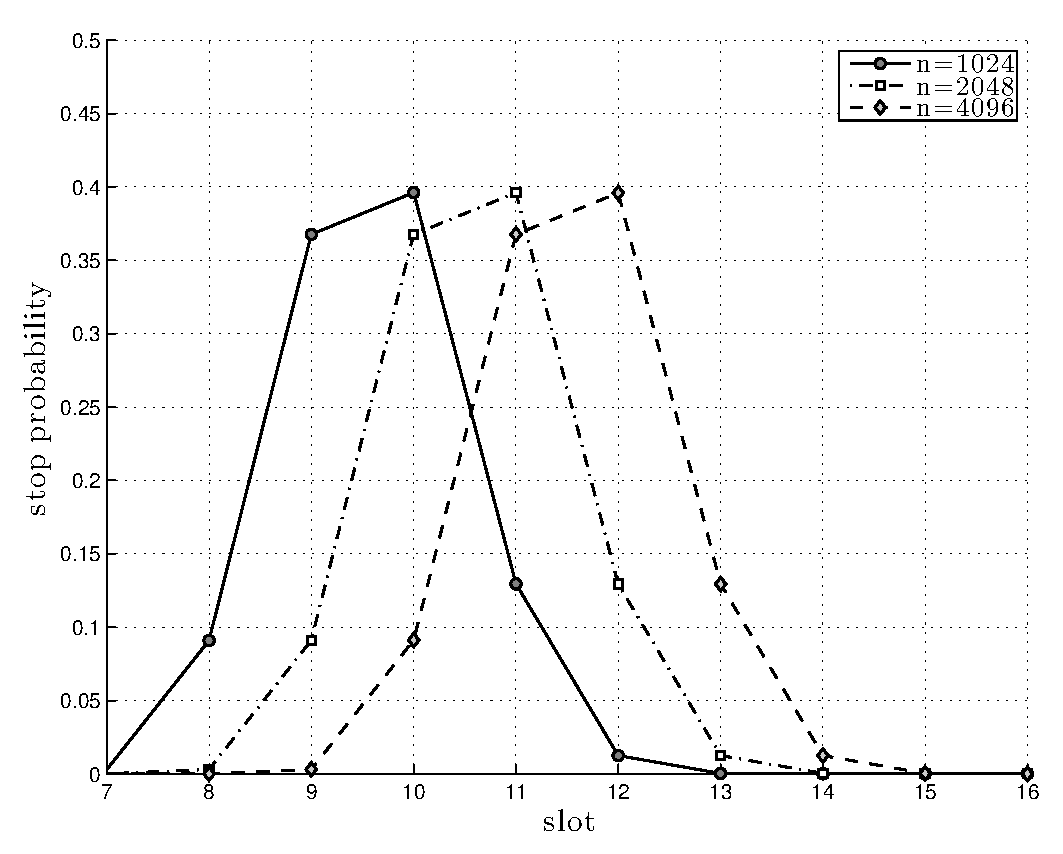
\epsfig{file=matlab/Greenberg_stop_prob/greenberg-stop-distribution-uniformity.eps,scale=0.7}
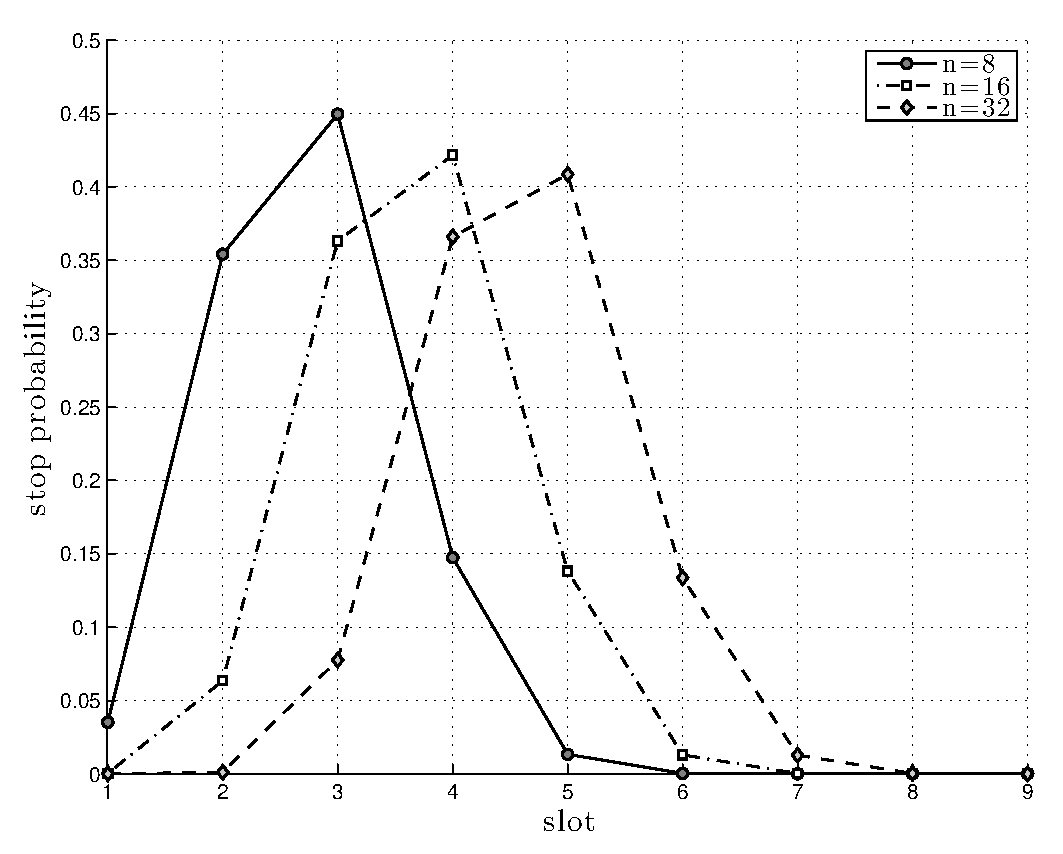
\includegraphics[width=0.7\textwidth]{matlab/Greenberg_stop_prob/greenberg-stop-distribution-uniformity-init}
\caption{\emph{Basic Greenberg}:  Small $2^{k}$ sizes distribution.}
\label{fig:greenberg-dist-small}
\end{center}
\end{figure}


\begin{figure}[H]
\begin{center}
%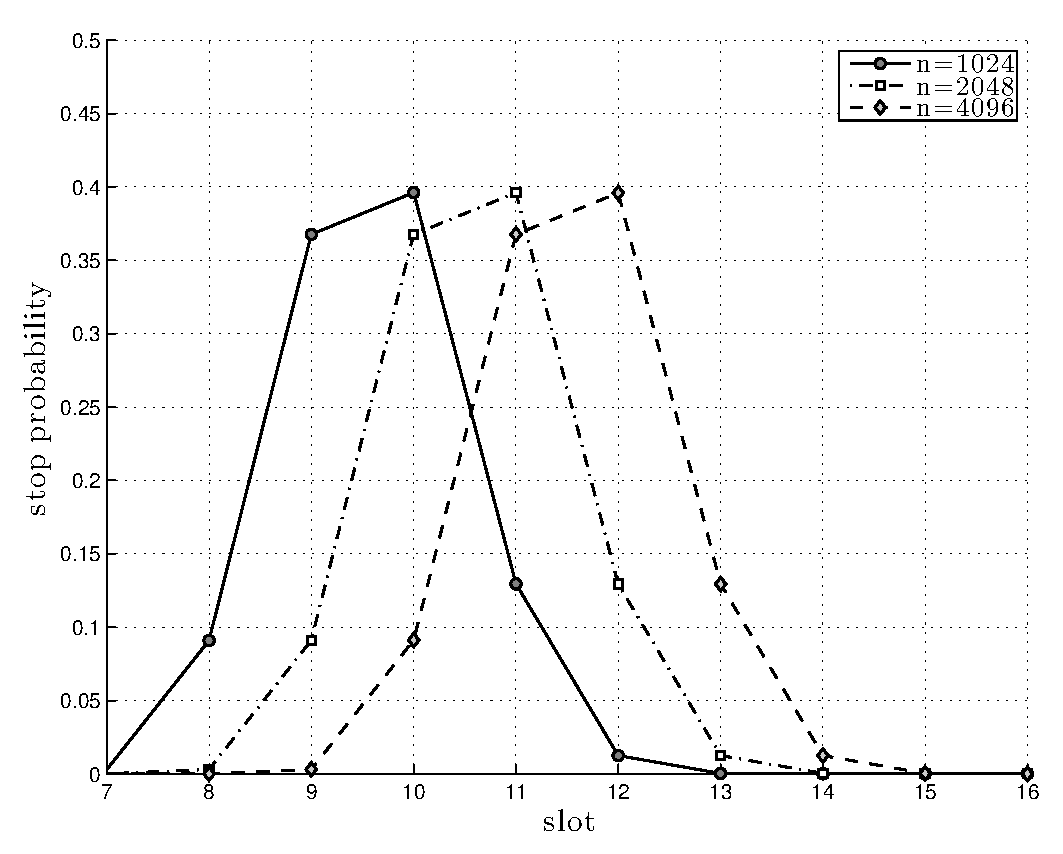
\epsfig{file=matlab/Greenberg_stop_prob/greenberg-stop-distribution-uniformity.eps,scale=0.7}
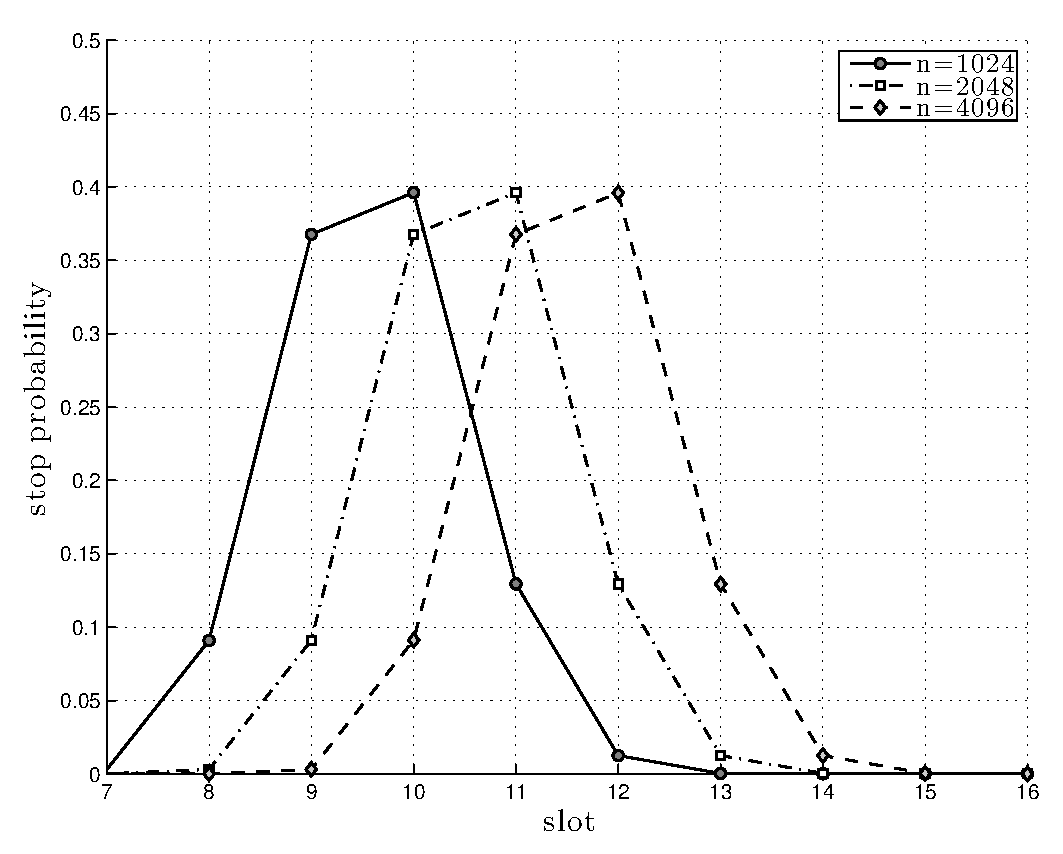
\includegraphics[width=0.7\textwidth]{matlab/Greenberg_stop_prob/greenberg-stop-distribution-uniformity}
\caption{\emph{Basic Greenberg}:  Large $2^{k}$ sizes distribution.}
\label{fig:greenberg-dist-large}
\end{center}
\end{figure}
An overview of the behavior of $\fg(n,i)$ is presented in Appendix in Table \ref{basic-greenberg-stop-probabilities} on page \pageref{basic-greenberg-stop-probabilities}.\\ Equation \eqref{eq:bgstopprobability} defines the probability for biased estimate $\hat{n}$ to be equal to $2^{i}$ when the batch size is $n$. 
\begin{equation}
\textrm{Pr}\left( \hat{n}=2^{i}|n\right)=\fg(n,i)  
\end{equation}

Figures \ref{fig:greenberg-dist-small} and \ref{fig:greenberg-dist-large} show how the distribution behaves respectively for small and large sizes.
We note that, for any fixed $n$, the distribution is well behaved with a bell-like shape. It turns out that, for batch sizes larger than 128, the distribution is ``stable'' in the sense that doubling the number of nodes produces only a shift of the stop probability of one slot to the right (see Figure \ref{fig:greenberg-dist-large} ).\\


\begin{figure}[htb]
\begin{center}
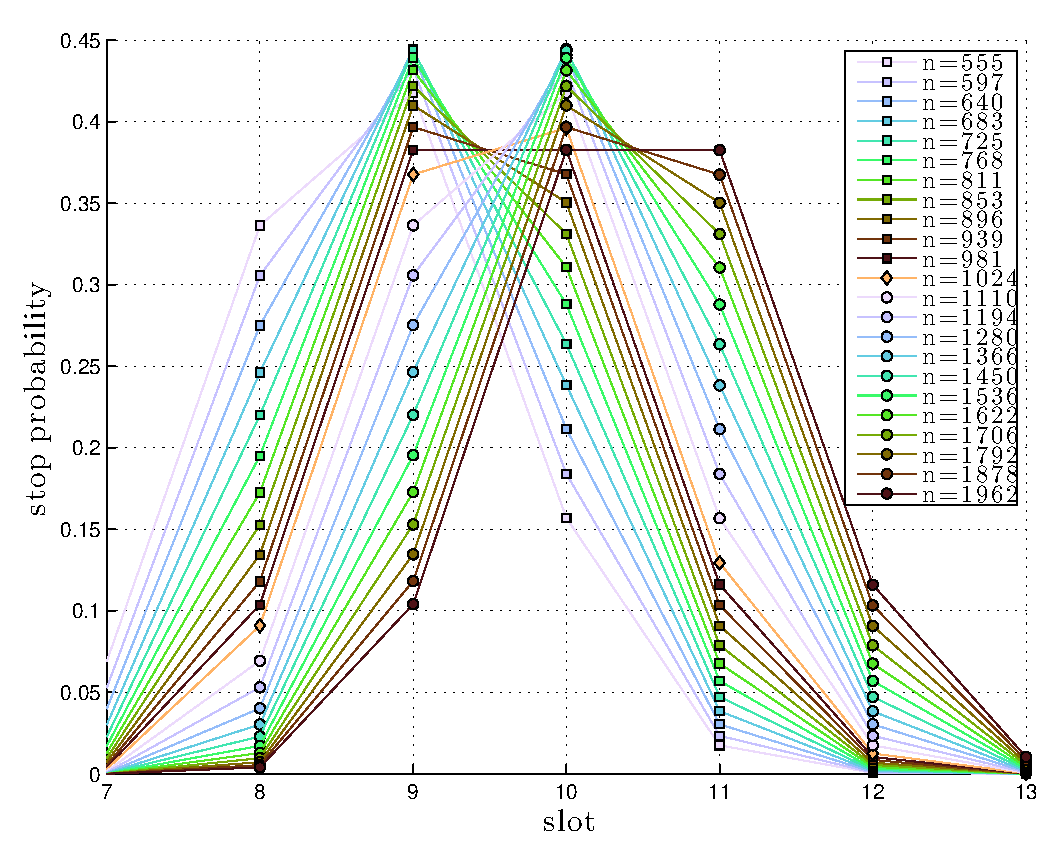
\includegraphics[width=0.85\textwidth]{matlab/Greenberg_stop_prob/greenberg-stop-distribution-intermediate-values}
\caption{\emph{Basic Greenberg}:  General batch sizes distribution.}
\label{fig:greenberg-dist-general}
\end{center}
\end{figure}
This is actually even for batch sizes that are not power of 2. Figure \ref{fig:greenberg-dist-general} shows the case.

%\subsection{Base $b$ Greenberg}
\subsection{Considerations}
Greenberg method is really good in terms of running time cost, which is $O\bigl(\log_{2}n\bigr)$. However it has some non negligible drawbacks:
\begin{enumerate}[\bf a)]
\item The estimation phase results in a sequence of colliding messages. These provide information about the cardinality of the batch, but do not help to solve an even small portion of the batch and can not carry auxiliary information. An algorithm that allows to get an estimate while resolving nodes would offer some advantages when the problem is not only the pure batch size estimation, but the batch resolution.
\item Basic Greenberg does not allow to achieve arbitrary precision in the estimate. In fact, we have that:
	\begin{enumerate}[\it i.]
		\item  the estimate is, by construction, a power of 2. Only a small subset of batch sizes can be mapped without error.
		\item the estimate distribution is not sharp enough around the correct value of the batch size but it spans over a few slots: this is shown in Figure \ref{fig:greenberg-dist-large}. We notice that using Greenberg algorithm it is difficult to discriminate between $n$ and $\frac{n}{2}$. 
	\end{enumerate}
\item Base $b$ Greenberg could  be used to get a tighter estimate. Anyway, to improve the accuracy, very small $b$ has to be choosen which results in much worse running times (see Table \ref{table:greenberg-b-phi}): even if theoretically it remains $O(log_{b}n)$ which is sublinear in $n$, in practice estimate time can even overwhelm $n$ when $b$ is small.
\end{enumerate}

\section{EGA BSE}
The \emph{Enhached Greenberg Algorithm (EGA)} is a first improvement over the Basic Greenberg algorithm. \\

Let $n$ be a batch size and $p$ be a given transmission probability. As expressed by \eqref{eq:greenberg-prob-empty} \eqref{eq:greenberg-prob-succ} \eqref{eq:greenberg-prob-coll}, varying $n$ while $p$ is fixed results in very different probabilities for \emph{idle}, \emph{successful} and \emph{collided} slots.

\begin{figure}[htbp]
\begin{center}
%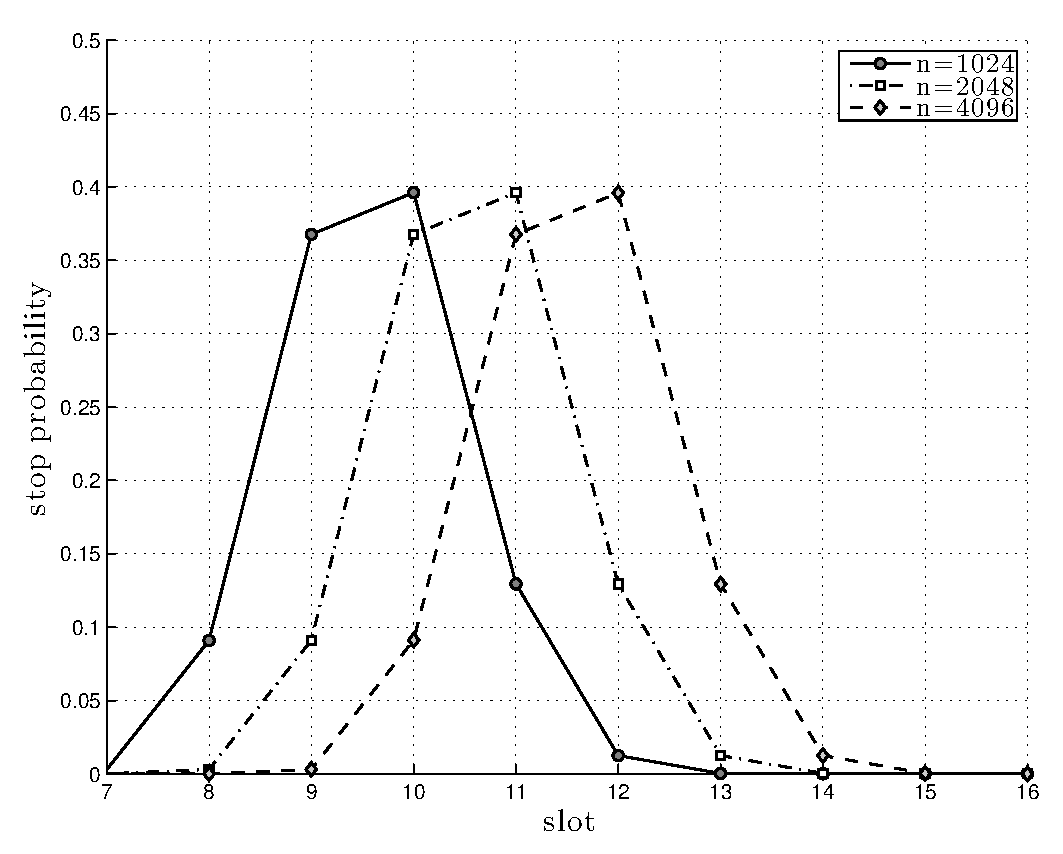
\epsfig{file=matlab/Greenberg_stop_prob/greenberg-stop-distribution-uniformity.eps,scale=0.7}
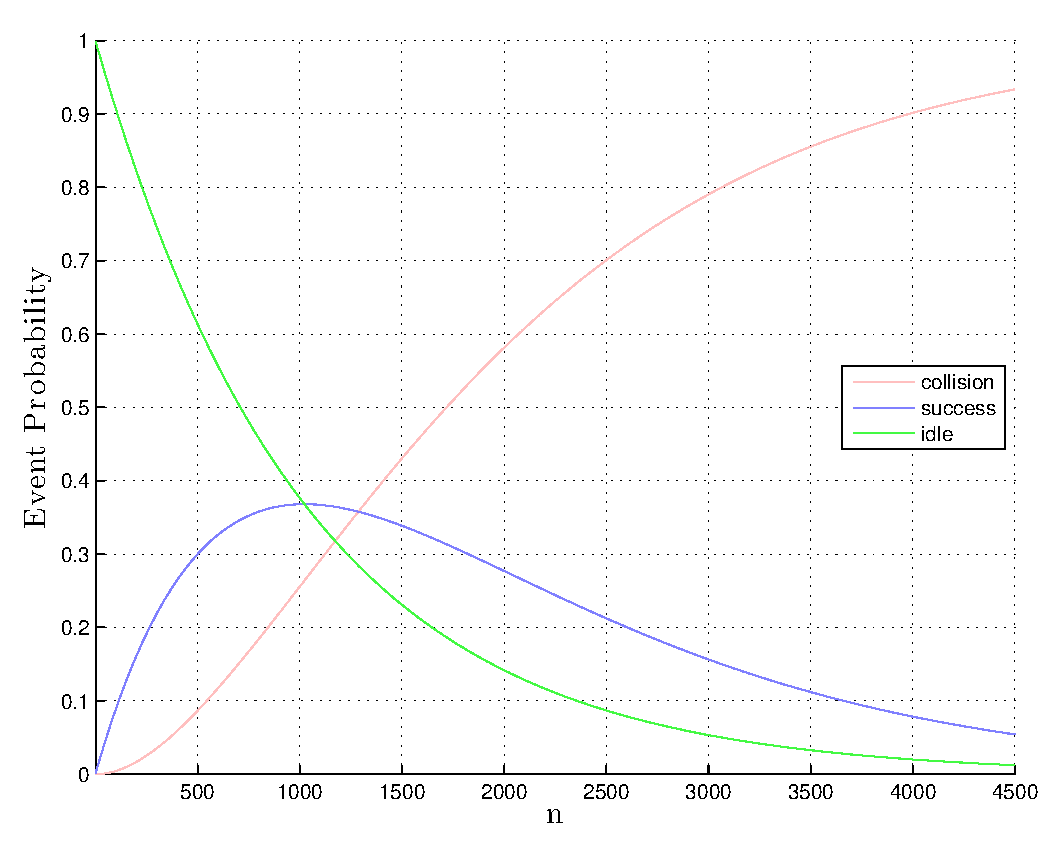
\includegraphics[width=0.7\textwidth]{matlab/Greenberg_MLE/draw_coll_idle_succ_fixed_p}
\caption[\emph{Basic Greenberg}: Event probability fixed $p$]{Probability of \emph{idle}, \emph{successful} or \emph{collided} slots varying $n$ while  $p=1/1024$.  $q_{0}(p,n) \approx  q_{1}(p,n)$ for $n=1023$}
\label{fg:event-prob-fixed-p-varying-n}
\end{center}
\end{figure}

Examining Figure \ref{fg:event-prob-fixed-p-varying-n}, it is quite immediate to see that:
\begin{itemize}
\item $q_{0}(p,n) \approx q_{1}(p,n)$ when $p\approx {\displaystyle\frac{1}{n}}$ and, obviously,
\item $q_{0}(p,n) \gg q_{1}(p,n)$ and $q_{0}(p,n) \gg q_{2+}(p,n)$ when $p \ll {\displaystyle\frac{1}{n}}$,
\item $q_{2+}(p,n) \gg q_{0}(p,n)$ and $q_{2+}(p,n) \gg q_{0}(p,n)$ when $p \gg {\displaystyle\frac{1}{n}}$.
\end{itemize}
The collision probability $q_{2+}(p,n)$ is strictly monotonic  increasing, while the empty slot probability $q_{0}(p,n)$ is strictly decreasing. Repeating a large number $T$ of transmission with  probability $p$, we can simply use the number of collisions or idle slots to uniquely determined the batch size. On the other hand, successful probability $q_{1}(p,n)$ is non-monotonic and hence can not be used to uniquely determine the batch size.\\
 
\noindent The proposed technique to refine the estimate is the following.\\
Running \emph{Basic Greenberg Algorithm} provides a raw estimate and the associated transmission probability $p$. Then we perform $T$ more transmissions and use a \emph{Maximum Likelihood Estimation (MLE)} to refine the estimate.\\ 
 
 Let $T$ be the number of slots we will use to refine the estimate and let $N_{0}$, $N_{1}$, $N_{2+}$ be random variables which represent the total number of idle, successful and collided slots, respectively, observed after the T additional slots.\\
 $N_{0}$, $N_{1}$, $N_{2+}$ are binomial distributions with parameters $B(n,q_{0}(p,n))$, $B(n,q_{1}(p,n))$ and $B(n,q_{2+}(p,n))$, respectively. Of course $N_{0}+N_{1}+N_{2+}=T$ and
 \begin{eqnarray*}
E[N_{0}] &=& Tq_{0}(p,n),\\
E[N_{1}] &=& Tq_{1}(p,n),\\
E[N_{2+}] &=& Tq_{2+}(p,n).
\end{eqnarray*}
Let $f_{T}(i,s,c,p',n')$ denote the probability to get $i$ idle, $s$ success and $c$ collision slots:
\begin{align}
\label{eg:Bettiol-test}
f_{T}(i,s,c,p',n')&= \textrm{Pr}(N_{0}=i,N_{1}=s,N_{2+}=c|n=n',p=p')\\
\nonumber
 &=\textrm{Pr}(N_{0}=i|n=n',p=p')\textrm{Pr}(N_{1}=s,N_{2+}=c|n=n',p=p',i),
\end{align}
when we transmit with probability $p'$ and the batch size is $n'$.\\
Let $\mathcal{N}$ be the set of the target batch sizes. Then, we can define
\begin{equation}
MLE(i,s,c,l) \gets \argmax_{\displaystyle{n' \in \mathcal{N}}} \Bigl( f_{T}\bigl(i,s,c,p(l),n')\cdot \fg\bigl(n',l\bigr)\Bigr).
\label{eq:MLEiscl}
\end{equation}
$MLE(i,s,c,l)$ is a $T \times T \times L$ matrix where $L$ is the index of the ``farthest'' slot that can be visited during the  \emph{Basic Greenberg Algorithm}. $L$ depends on the maximum cardinality  $n_{max}$ considered for the problem. Consequently  $L$ must be chosen so not to worse the performance of our estimator (if $n_{max}$ is smaller than the real batch size $n$) and not to waste too much memory.\\
Hence, our estimate is simply the result of a look-up in the $MLE$ table,
\begin{equation}
\hat{n} \longleftarrow MLE(i,s,c,l).
\end{equation}
Is it worth mentioning that:
\begin{itemize}
\item  For performance tuning, the $MLE$ table can be precomputed before running the estimate algorithm. The computational cost to fill the whole $MLE$ table depends on $T$ and $L$ and, if trivial exhaustive search on $\mathcal{N}$ is performed, also on $|\mathcal{N}|$. A fast way to compute the MLE table is described in Section \ref{sc:GEGA BSE}.
\item The size of the $MLE$ table does not depend on $|\mathcal{N}|$ but only on $T$ and $L$.
\item The estimate deeply depends on the way the elements in $\mathcal{N}$ are chosen. \\
\end{itemize}

The high level pseudo-code of the algorithm is the following: 
\begin{algorithm}[H]
\begin{algorithmic}
\STATE precompute or load the $MLE$ table characterized by $T$, $L$, $\mathcal{N}$
\STATE $l\gets 0$
\REPEAT
	\STATE $l\gets l+1$
	\STATE $p \gets {\displaystyle\frac{1}{2^{l}}}$
	\STATE choose to transmit with probability $p$
\UNTIL {no collision occurs}
\STATE $(i,s,c) \gets$ events resulting from $T$ transmissions with probability $p$
\STATE $\hat{n}\gets MLE(i,s,c,l)$
\end{algorithmic}
\caption{\algname{EGA $(\mathcal{B},T,\mathcal{N})$}}
\label{alg-greenberg+MLE}
\end{algorithm}
Expected running time in slots follows from Greenberg expected running time and the further used slots. Therefore expected slot cost is is $\approx \log_{2}n+T$.\\ 
We note also that only $MLE(i,s,c,l)$ is involved by the algorithm and not the whole $MLE$ table. Hence, is it possible to choose wheter precomputing and storing the whole table or computing only $MLE(i,s,c,l)$ on-demand.\\
Once both the batch size $n$ and the $MLE$ table are fixed, the probability to estimate $\hat{n}$ can be expressed as:
\begin{equation}
\textrm{Pr}(\hat{n}=n'|n)=\sum_{l}\fg(n,l)\sum_{i}\sum_{s} \hat{X}_{MLE(i,s,c,l)}(n') \cdot f_{T}\big(i,s,c,p(l),n\bigl),
\end{equation}
 where  $\hat{X}_{MLE(i,s,c,l)}(n')=1$ iff $MLE(i,s,c,l)=n'$,  $\hat{X}_{MLE(i,s,c,l)}(n')=0$ otherwise. \\
Hence the expected value of the estimate given $n$ can be trivially computed as follows:
\begin{equation}
E[\hat{n}|n]=\sum_{n'\in\,\mathcal{N}}n'\cdot\textrm{Pr}(\hat{n}=n'|n).
\label{eq:EGA expected estimate given n}
\end{equation}
 
\begin{comment}
\begin{figure}[H]
\begin{center}
\includegraphics[width=0.7\textwidth]{matlab/Greenberg_MLE/greenberg-mle-T10}
\caption{\emph{EGA}: PROVVISORIO $T=10$  power of 2 distribution.}
\end{center}
\end{figure}
\end{comment}

\subsection{Performance}
\begin{figure}[H]
\begin{center}
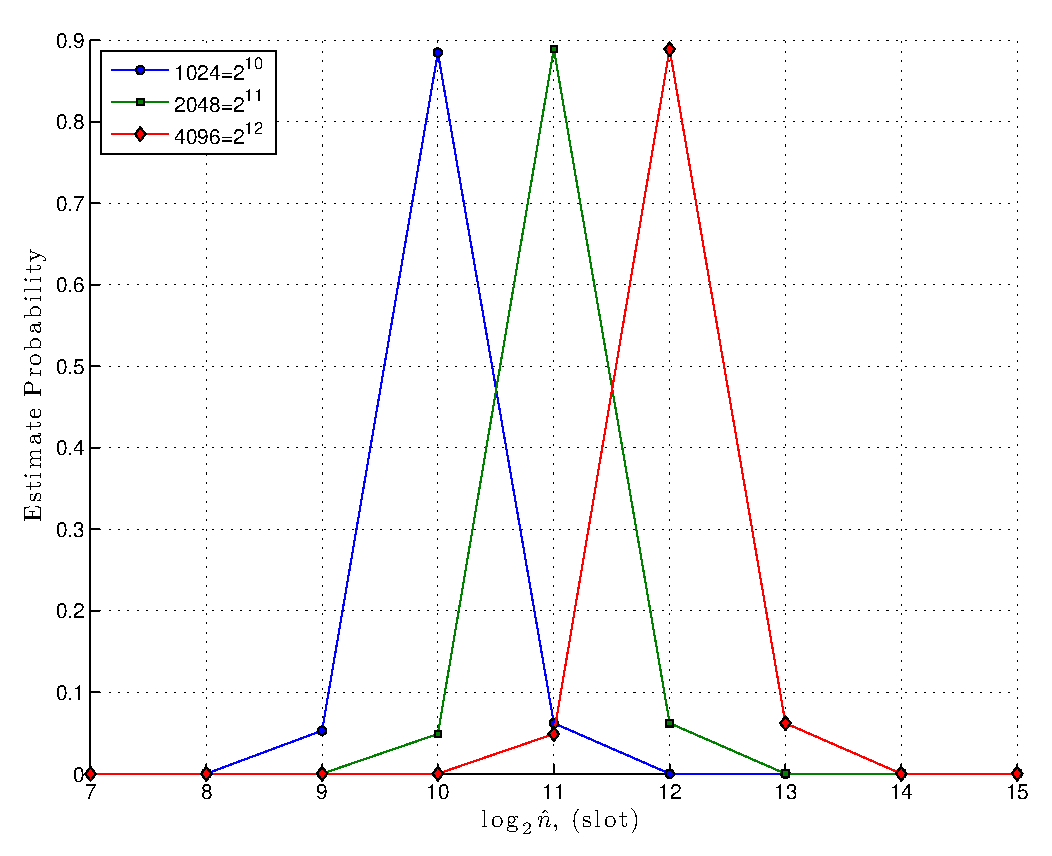
\includegraphics[width=0.7\textwidth]{matlab/Greenberg_MLE/greenberg-mle-T20}
\caption{\emph{EGA}:  Large $2^{k}$ sizes distribution.}
\label{fg:EGA-sharp-peaks}
\end{center}
\end{figure}

\begin{figure}[H]
\begin{center}
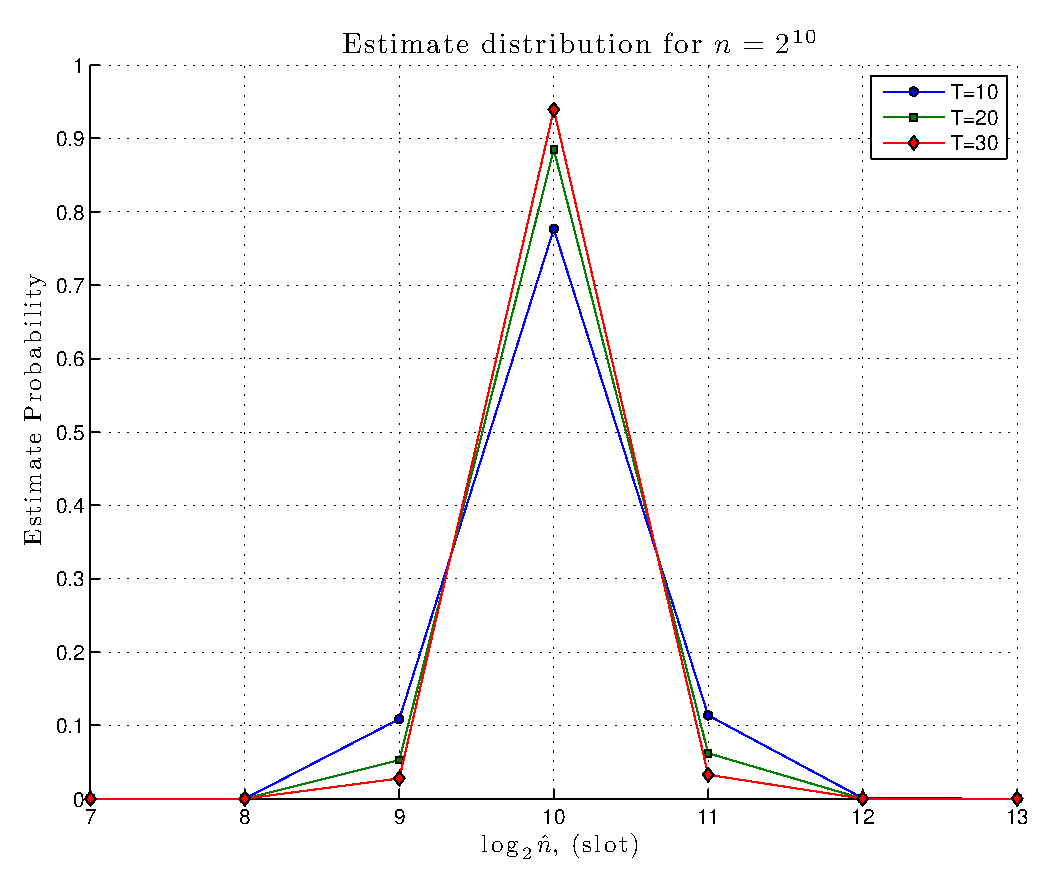
\includegraphics[width=0.7\textwidth]{matlab/Greenberg_MLE/greenberg-mle-fixed-n-varying-T}
\caption[\emph{EGA}: Estimate distribution when varying $T$.]{\emph{EGA}: Estimate distribution when varying $T$. Plot refers to $n=1024$.}
\label{fg:EGA-peaks-fixed-n-varing-T}
\end{center}
\end{figure}
Figures in this section were obtained by considering $\mathcal{N}=\{\textrm{powers of 2}\}$. Therefore, the target estimates are the same as for \emph{basic Greenberg algorithm}.\\
Figure \ref{fg:EGA-sharp-peaks} shows that the proposed method peaks sharply near the right estimate. Comparing to the basic Greenberg method (see Figure \ref{fig:greenberg-dist-large}) you can notice that there is only one extremely sharp peak located in a single slot, instead of a bell-like shape distributed among consecutive slots. Furthermore, you can also notice how the probability to overestimate the batch size is a bit higher than the probability to underestimate it.\\
Figure \ref{fg:EGA-peaks-fixed-n-varing-T} shows how the peak behaves when varying $T$ for a fixed batch size: increasing $T$ the peak becomes more and more sharp.
%\clearpage
\section{GEGA BSE}
\label{sc:GEGA BSE}
The  \emph{Generalized Enhanced Greenberg Algorithm (GEGA)} is a less restrictive form of the EGA algorithm in the sense that we do not  limit \emph{a priori} the set  of target estimates. This can be simply achieved by letting $\mathcal{N}$ be the set of all the positive integer numbers.
\begin{equation*}
\mathcal{N}=\{1,2,3,...\}.
\end{equation*}
In this case the algorithm can be interpreted as follows:
\begin{enumerate}
\item Find the transmission probability $p$ for which the multiplicity of the activated set is 1 with very high probability,
\item Use $T$ consecutive slots (a ``window'') to refine the estimate. The idea is similar to a window based estimate except that a node is allowed to transmit in each slot.
\end{enumerate}

\noindent Recalling \eqref{eq:MLEiscl}, given $i$, $s$, $c$ and $l$, the estimate can be found by solving:
\begin{equation}
\frac{d\Bigl( f_{T}\bigl(i,s,c,p(l),n)\cdot \fg\bigl(n,l\bigr)\Bigr)}{dn}=0,
\end{equation}
which is not trivial to solve and involves numerical problems since $\fg(n,l)$ can present very small product terms. Then we solved the problem by using bisection method on  \eqref{eq:MLEiscl} and taking the largest integer $n$ for which
\begin{equation}
f_{T}\bigl(i,s,c,p(l),n+1)\cdot \fg\bigl(n+1,l\bigr)-f_{T}\bigl(i,s,c,p(l),n)\cdot \fg\bigl(n,l\bigr)\geq0.
\end{equation}
As an example, the results of this computation when $T=10$ and $l=10$ are presented in Table \ref{tb:GEGA-T10-l10}.

\begin{table}[htbp]
\centering
\resizebox{0.8\textwidth}{!}{
\begin{tabular}{|r|l|l|l|l|l|l|l|l|l|l|l|}
\hline
\backslashbox{$c$}{$s$} & \multicolumn{1}{r|}{0} & \multicolumn{1}{r|}{1} & \multicolumn{1}{r|}{2} & \multicolumn{1}{r|}{3} & \multicolumn{1}{r|}{4} & \multicolumn{1}{r|}{5} & \multicolumn{1}{r|}{6} & \multicolumn{1}{r|}{7} & \multicolumn{1}{r|}{8} & \multicolumn{1}{r|}{9} & \multicolumn{1}{r|}{10} \\ \hline
0 & 352 & 413 & 477 & 545 & 616 & 689 & 765 & 843 & 922 & 1003 & 1086 \\ \hline
1 & 489 & 559 & 632 & 709 & 787 & 868 & 951 & 1036 & 1122 & 1210 & - \\ \hline
2 & 650 & 730 & 812 & 896 & 983 & 1072 & 1162 & 1254 & 1347 & - & - \\ \hline
3 & 838 & 927 & 1017 & 1111 & 1206 & 1302 & 1401 & 1501 & - & - & - \\ \hline
4 & 1055 & 1153 & 1254 & 1356 & 1461 & 1567 & 1675 & - & - & - & - \\ \hline
5 & 1307 & 1416 & 1527 & 1641 & 1757 & 1875 & - & - & - & - & - \\ \hline
6 & 1603 & 1726 & 1851 & 1979 & 2110 & - & - & - & - & - & - \\ \hline
7 & 1962 & 2103 & 2248 & 2396 & - & - & - & - & - & - & - \\ \hline
8 & 2416 & 2585 & 2761 & - & - & - & - & - & - & - & - \\ \hline
9 & 3044 & 3267 & - & - & - & - & - & - & - & - & - \\ \hline
10 & 4111 & - & - & - & - & - & - & - & - & - & - \\ \hline
\end{tabular}
}
\caption{\emph{GEGA}: Possible estimates when $T=10$ and $l=10$.}
\label{tb:GEGA-T10-l10}
\end{table}

Table \ref{tb:GEGA-T10-l10} reveals that the estimate is always finite. This good feature  follows from the bounded moments of the Greenberg algorithm. In general (see Table \ref{tb:window-estimate}), simple window based MLE estimators can not achieve finite estimate when all the events are collisions.\\

The EGA MLE Table defined in \eqref{eq:MLEiscl} can be obtained as sub-case from GEGA MLE Table. In fact, once the GEGA MLE Table has been computed,  for each tuple ($i$,$s$,$c$,$l$) providing estimate $n'$, the corresponding EGA estimate can be obtained by considering the closest two EGA target estimates surrounding $n'$ and by taking the best between the two by using \eqref{eq:MLEiscl} as usual. Even more, since extensive computation of the  GEGA MLE can take really long time, it is worth to mention that computation can be speed up looking only for solutions which satisfy the following constrain:\\
\begin{equation}
\max(MLE(T-s-c,s-1,c,l),MLE(T-s-c,s,c-1,l))\leq MLE(i,s,c,l)
\label{eq:speedup}
\end{equation}

This simply means that computing Table \ref{tb:GEGA-T10-l10} cells  by diagonal can benefit of \ref{eq:speedup} and speed up the computation process.

\clearpage
\subsection{Performance}

The estimate provided by GEGA is biased. Figure \ref{fg:GEGA-bias} shows that the algorithm tends to overestimate the real batch size. Anyway, the bias can be easily corrected since it is always really near to the average value: the oscillations have very small amplitude. Increasing $T$ reduces the bias as well as the oscillations amplitude. Very small batch sizes (less than 20) show higher oscillations compared to larger ones: this fact is negligible in practice since the oscillations are too small to affect the estimate and are hidden by the rounding operation. Table \ref{tb:GEGA-average-bias} reports the average bias $\phi(T)$ as a function of $T$. 
\begin{figure}[hb]
\makebox[\textwidth][c]{% exchange [l] with [r] or [c] to extend it into the left border or both, respectively
  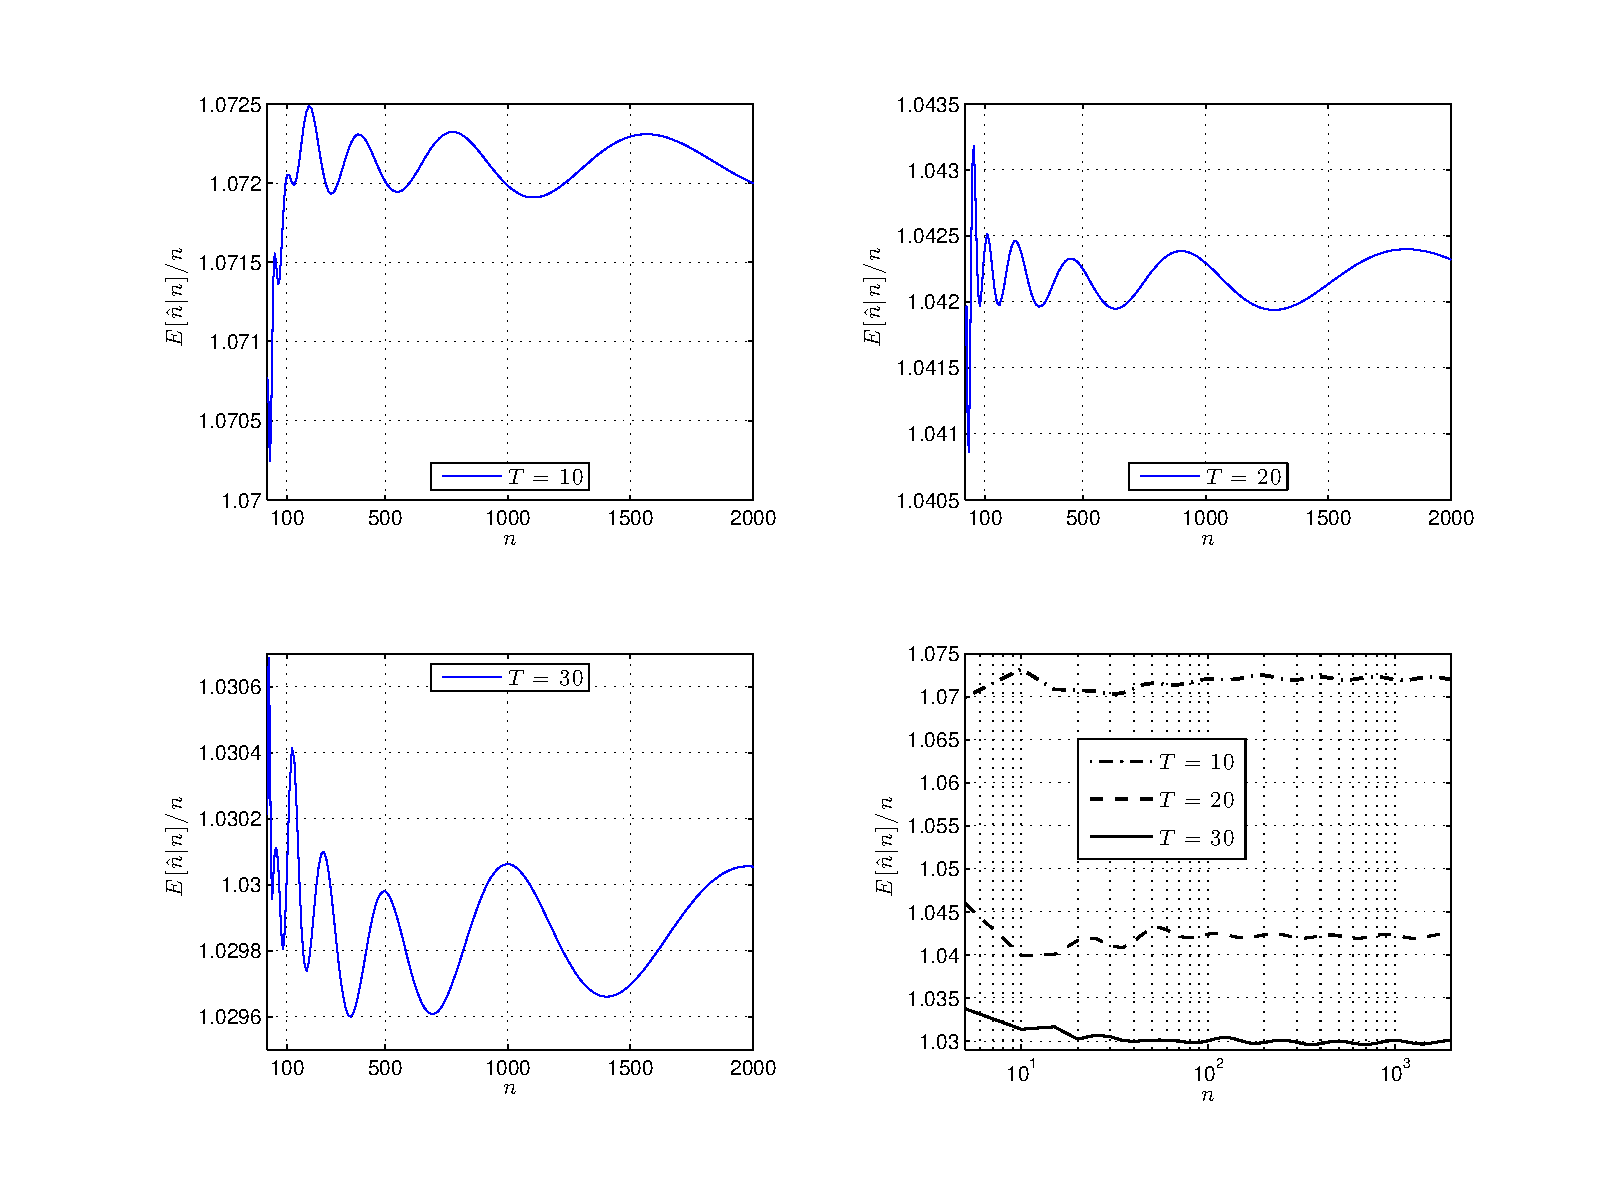
\includegraphics[width=1.2\textwidth]{matlab/GEGA/GEGA-bias-varying-T}% here 20% wider than \textwidth
 }
\caption[\emph{GEGA}: Estimate Bias]{\emph{GEGA}: Estimate Bias. The first tree plots show the estimate expected value over the real batch size for different $T$. Right below corner plot provides a summary in a log x-scale. Data reported were computed using formula \eqref{eq:EGA expected estimate given n}.}
\label{fg:GEGA-bias}
\end{figure}

The results where computed by averaging the bias estimate for batch sizes from 2 to 2000.\\ 

\begin{table}[htdp]
\centering
\begin{tabular}{c|c}
\toprule
$T$ & $\phi(T)$ \\
\midrule
10 & 0.0723  \\
20 & 0.0422  \\
30 & 0.0299\\
\bottomrule
\end{tabular} 
\caption{\emph{GEGA}: Average bias.}
\label{tb:GEGA-average-bias}
\end{table}

\begin{figure}[h]
\makebox[\textwidth][c]{% exchange [l] with [r] or [c] to extend it into the left border or both, respectively
    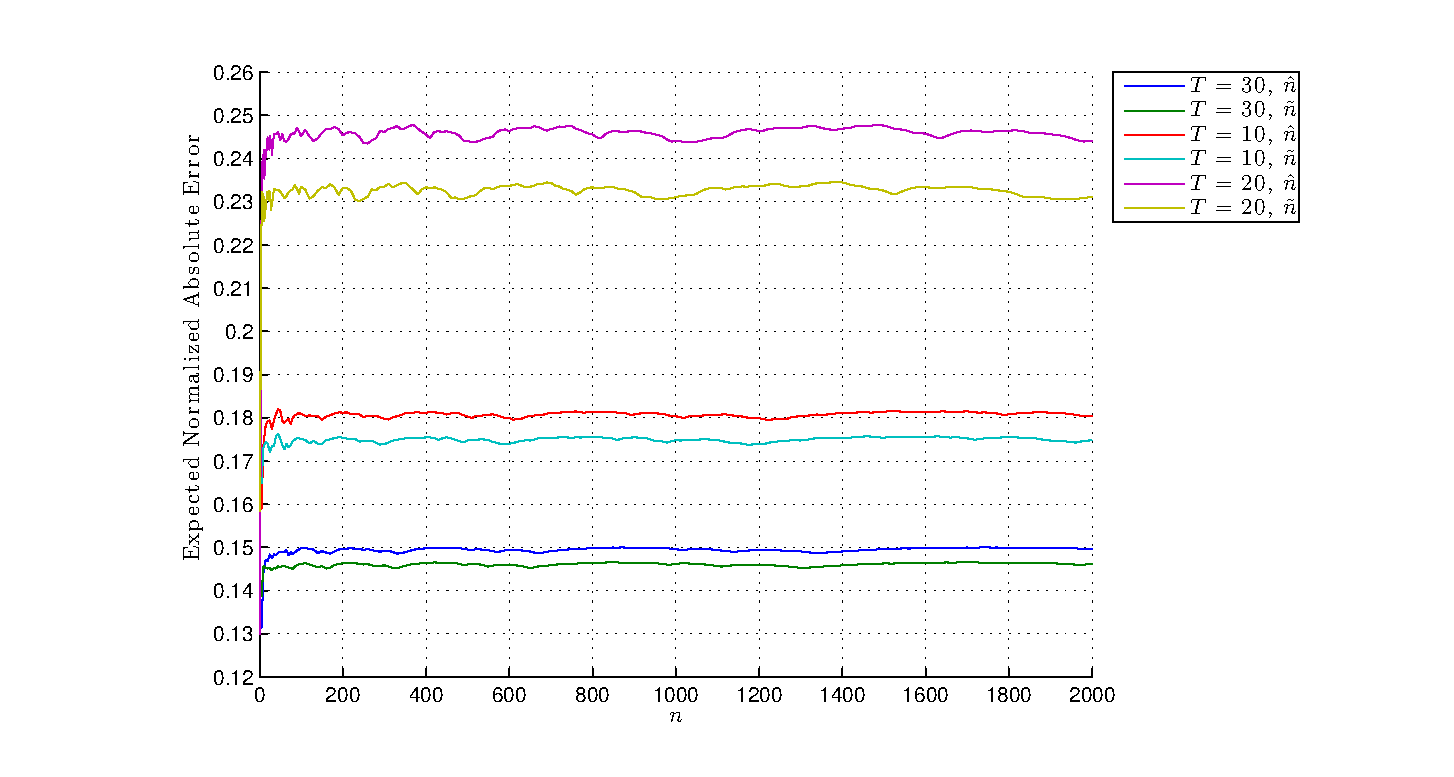
\includegraphics[width=1.2\textwidth]{matlab/GEGA/GEGA-bias-unbias-absolute-normalized-error}% here 20% wider than \textwidth
 }
 \caption[\emph{GEGA}: Biased/unbiased absolute normalized estimate error]{\emph{GEGA}: biased/unbiased absolute normalized estimate error. The plot presents $e(\hat{n})$ and $e(\tilde{n})$ for different $T$.}
 \label{fg:GEGA-biased-unbiased}
\end{figure}

Estimate bias can be corrected by considering $\tilde{n}={\displaystyle \frac{\hat{n}}{\phi(T)+1}}$. We will see that in this way we get higher quality estimate.\\
To measure the performance of the proposed estimation method, we define the normalized absolute estimate error as
\begin{equation}
e(\hat{n})=\frac{|\hat{n}-n|}{n}.
\label{GEGA-abs-error}
\end{equation}
In the same manner we can define $e(\tilde{n})$. The parameter $T$ is implicitly present in \eqref{GEGA-abs-error}.
Figure \ref{fg:GEGA-biased-unbiased} shows that the bias-corrected estimate performs better than the biased estimate for any batch size and $T$. Furthermore, you can notice that the error is independent of the batch size.  
\begin{figure}[H]
\centering
    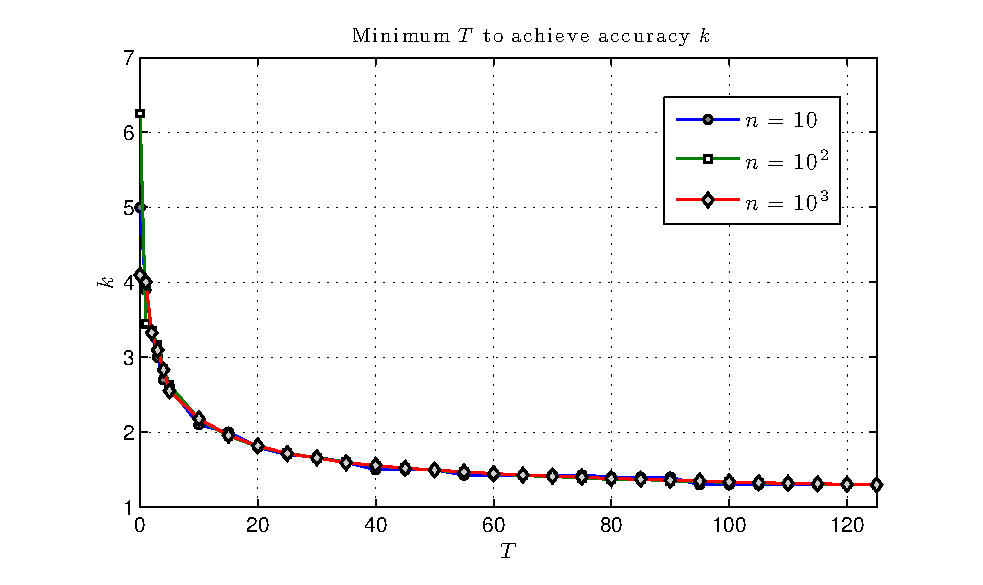
\includegraphics[width=0.8\textwidth,height=0.3\textheight]{matlab/GEGA/GEGA-min-T-for-k}% here 20% wider than \textwidth
 \caption{\emph{GEGA}: Minimum $T$ to achieve error coefficient lower than $k$ with $\theta=0.99$}
 \label{fg:GEGA-min-T-for-k}
\end{figure}

\begin{figure}[H]
\centering
    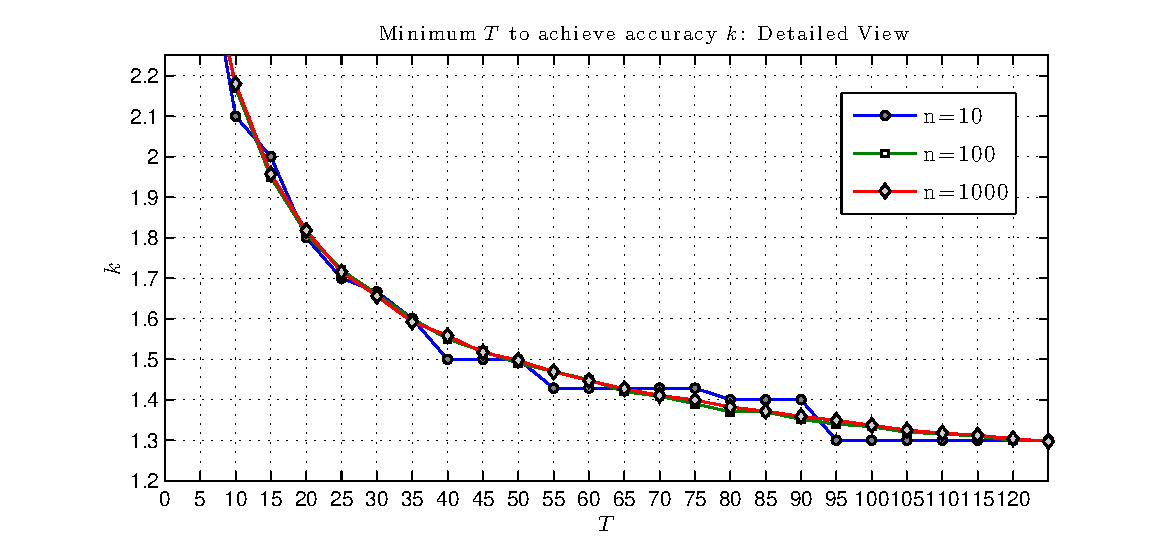
\includegraphics[width=0.8\textwidth,height=0.3\textheight]{matlab/GEGA/GEGA-min-T-for-k-detail}% here 20% wider than \textwidth
 \caption{\emph{GEGA}: Minimum $T$ to achieve error coefficient lower than $k$ with $\theta=0.99$ , detailed view}
 \label{fg:GEGA-min-T-for-k-detail}
\end{figure}
Results presented in Figures  \ref{fg:GEGA-min-T-for-k} and  \ref{fg:GEGA-min-T-for-k-detail} show that the accuracy in the estimate grows as $T$ increases and it is independent of the batch size when the batch size is not too small (e.g.: $n=10$). In fact, for very small batch sizes, the error coefficient $k$ shows a descending steps trend since the  probability distribution is discrete and the adopted algorithm performs rounding operations. Furthermore, it is important to mention that $T$ allows the user to choose estimate accuracy easily, without caring about the batch size. In other words, if we require a given estimate accuracy, in terms of error coefficient $k$, the minimum necessary $T$ can be easily determined looking at Figure  \ref{fg:GEGA-min-T-for-k-detail}.

%\clearpage
\section{Comparison}
Here we will provide the reader a comparison between the estimates obtained using \emph{Cidon} and \emph{GEGA} algorithms in terms of accuracy and time. In fact, in real life scenarios, we will be interested in getting a ``tight enough'' estimate of the real batch size in a reasonable time. We must always remember that there is a trade-off between the time taken by an explicit estimate phase and the following resolution: the goal is to minimize the total cost.\\ For the comparison we considered the dynamically  adapting versions of the described algorithms:
\begin{itemize}
\item in \emph{Cidon} this means that $\pc$ is not \emph{a priori} fixed but, as the resolution goes on, gets updated in accordance to the resolved interval.
\item in \emph{GEGA} this simply means that $T$ grows as the elapsed time.
\end{itemize}
\begin{figure}[h]
\centering
% !TEX root = ../tesi.tex
% This file was created by matlab2tikz v0.0.6.
% Copyright (c) 2008--2010, Nico Schlömer <nico.schloemer@gmail.com>
% All rights reserved.
% 
% The latest updates can be retrieved from
%   http://www.mathworks.com/matlabcentral/fileexchange/22022-matlab2tikz
% where you can also make suggestions and rate matlab2tikz.
% 
\begin{comment}
\begin{tikzpicture}

% defining custom colors

\definecolor{mycolor1}{rgb}{0,0.5,0}
\definecolor{mycolor2}{rgb}{0,0.75,0.75}
\definecolor{mycolor3}{rgb}{0.75,0,0.75}
\definecolor{mycolor4}{rgb}{0.75,0.75,0}


\begin{axis}[
        xlabel=Elapsed time in slots,
        ylabel=$k$ accuracy
	view={0}{90},
	scale only axis,
	width=4.82222in,
	height=3.80333in,
	xmin=0, xmax=100,
	ymin=1, ymax=7,
	xtick={0,10,20,30,40,50,60,70,80,90,100},
	ytick={0,0.5,1,1.5,2,2.5,3,3.5,4,4.5,5,5.5,6,6.5,7,7.5,8},
	yticklabels={1,1.5,2,2.5,3,3.5,4,4.5,5,5.5,6,6.5,7},
	xlabel={Elapsed time in slots},
	ylabel={$k$ accuracy},
	xmajorgrids,
	ymajorgrids,
	legend entries={Cidon \ $n=10$,Cidon \ $n=10^{2}$,Cidon \ $n=10^{3}$,GEGA $n=10$,GEGA $n=10^{2}$,GEGA $n=10^{3}$},
	legend style={nodes=right},
	mark repeat=15
    ]
\addplot [
color=blue, const plot
]
coordinates{ (9.7051,3.7) (9.79253,3.7) (9.87997,3.7) (9.9674,3.7) (10.0548,3.7) (10.1423,3.7) (10.2297,3.7) (10.3171,3.7) (10.4046,3.7) (10.492,3.7) (10.5794,3.7) (10.6669,3.7) (10.7543,3.7) (10.8417,3.7) (10.9292,3.7) (11.0166,3.7) (11.104,3.7) (11.1915,3.7) (11.2789,3.7) (11.3663,3.7) (11.4538,3.7) (11.5412,3.7) (11.6286,3.7) (11.7161,3.7) (11.8035,3.7) (11.8909,3.7) (11.9784,3.7) (12.0658,3.7) (12.1532,3.7) (12.2407,3.7) (12.3281,3.7) (12.4155,3.7) (12.503,3.7) (12.5904,3.7) (12.6778,3.7) (12.7653,3.7) (12.8527,3.7) (12.9401,3.7) (13.0276,3.7) (13.115,3.7) (13.2024,3.7) (13.2899,2.53333) (13.3773,2.53333) (13.4647,2.53333) (13.5522,2.53333) (13.6396,2.53333) (13.727,2.53333) (13.8145,2.53333) (13.9019,2.53333) (13.9893,2.53333) (14.0768,2.53333) (14.1642,2.53333) (14.2516,2.53333) (14.3391,2.53333) (14.4265,2.53333) (14.5139,2.53333) (14.6014,2.53333) (14.6888,2.53333) (14.7762,2.53333) (14.8637,2.53333) (14.9511,2.53333) (15.0385,2.53333) (15.126,2.53333) (15.2134,2.53333) (15.3008,2.53333) (15.3883,2.53333) (15.4757,2.53333) (15.5631,2.53333) (15.6506,2.53333) (15.738,2.53333) (15.8254,2.53333) (15.9129,2.53333) (16.0003,2.53333) (16.0877,2.04444) (16.1752,2.04444) (16.2626,2.04444) (16.35,2.04444) (16.4375,2.04444) (16.5249,2.04444) (16.6123,2.04444) (16.6998,2.04444) (16.7872,2.04444) (16.8746,2.04444) (16.9621,2.04444) (17.0495,2.04444) (17.1369,2.04444) (17.2244,2.04444) (17.3118,2.04444) (17.3992,2.04444) (17.4867,2.04444) (17.5741,2.04444) (17.6615,2.04444) (17.749,2.04444) (17.8364,2.04444) (17.9238,2.04444) (18.0113,2.04444) (18.0987,2.04444) (18.1861,2.04444) (18.2736,2.04444) (18.361,2.04444) (18.4484,1.75833) (18.5359,1.75833) (18.6233,1.75833) (18.7107,1.75833) (18.7982,1.75833) (18.8856,1.75833) (18.973,1.75833) (19.0605,1.75833) (19.1479,1.75833) (19.2353,1.75833) (19.3228,1.75833) (19.4102,1.75833) (19.4976,1.75833) (19.5851,1.75833) (19.6725,1.75833) (19.7599,1.75833) (19.8474,1.75833) (19.9348,1.75833) (20.0222,1.75833) (20.1097,1.75833) (20.1971,1.75833) (20.2845,1.75833) (20.372,1.75833) (20.4594,1.75833) (20.5468,1.56667) (20.6343,1.56667) (20.7217,1.56667) (20.8091,1.56667) (20.8966,1.56667) (20.984,1.56667) (21.0714,1.56667) (21.1589,1.56667) (21.2463,1.56667) (21.3337,1.56667) (21.4212,1.56667) (21.5086,1.56667) (21.596,1.56667) (21.6835,1.56667) (21.7709,1.56667) (21.8583,1.56667) (21.9458,1.56667) (22.0332,1.56667) (22.1206,1.56667) (22.2081,1.56667) (22.2955,1.41667) (22.3829,1.41667) (22.4704,1.41667) (22.5578,1.41667) (22.6452,1.41667) (22.7327,1.41667) (22.8201,1.41667) (22.9075,1.41667) (22.995,1.41667) (23.0824,1.41667) (23.1698,1.41667) (23.2573,1.41667) (23.3447,1.41667) (23.4321,1.41667) (23.5196,1.41667) (23.607,1.41667) (23.6944,1.41667) (23.7819,1.41667) (23.8693,1.3) (23.9567,1.3) (24.0442,1.3) (24.1316,1.3) (24.219,1.3) (24.3065,1.3) (24.3939,1.3) (24.4813,1.3) (24.5688,1.3) (24.6562,1.3) (24.7436,1.3) (24.8311,1.3) (24.9185,1.3) (25.0059,1.19167) (25.0934,1.19167) (25.1808,1.19167) (25.2682,1.19167) (25.3557,1.19167) (25.4431,1.19167) (25.5305,1.19167) (25.618,1.19167) (25.7054,1.19167) (25.7928,1.19167) (25.8803,1.0963) (25.9677,1.0963) (26.0551,1.0963) (26.1426,1.0963) (26.23,1)
};

\addplot [
color=mycolor1,
]
coordinates{ (12.1179,4.61988) (12.5668,4.61988) (13.0156,4.61988) (13.4644,4.61988) (13.9132,4.61988) (14.362,4.61988) (14.8108,4.61988) (15.2596,4.61988) (15.7084,4.61988) (16.1573,4.61988) (16.6061,4.61988) (17.0549,3.25103) (17.5037,3.25103) (17.9525,3.25103) (18.4013,3.25103) (18.8501,3.25103) (19.299,3.25103) (19.7478,3.25103) (20.1966,3.25103) (20.6454,3.25103) (21.0942,3.25103) (21.543,2.73771) (21.9918,2.73771) (22.4406,2.73771) (22.8895,2.73771) (23.3383,2.73771) (23.7871,2.73771) (24.2359,2.73771) (24.6847,2.73771) (25.1335,2.73771) (25.5823,2.43827) (26.0311,2.43827) (26.48,2.43827) (26.9288,2.43827) (27.3776,2.43827) (27.8264,2.43827) (28.2752,2.43827) (28.724,2.43827) (29.1728,2.43827) (29.6216,2.25861) (30.0705,2.25861) (30.5193,2.25861) (30.9681,2.25861) (31.4169,2.25861) (31.8657,2.25861) (32.3145,2.25861) (32.7633,2.25861) (33.2122,2.11032) (33.661,2.11032) (34.1098,2.11032) (34.5586,2.11032) (35.0074,2.11032) (35.4562,2.11032) (35.905,2.11032) (36.3538,2.11032) (36.8027,2.00439) (37.2515,2.00439) (37.7003,2.00439) (38.1491,2.00439) (38.5979,2.00439) (39.0467,2.00439) (39.4955,2.00439) (39.9443,2.00439) (40.3932,1.92495) (40.842,1.92495) (41.2908,1.92495) (41.7396,1.92495) (42.1884,1.92495) (42.6372,1.92495) (43.086,1.92495) (43.5348,1.92495) (43.9837,1.86316) (44.4325,1.86316) (44.8813,1.86316) (45.3301,1.86316) (45.7789,1.86316) (46.2277,1.86316) (46.6765,1.86316) (47.1253,1.79662) (47.5742,1.79662) (48.023,1.79662) (48.4718,1.79662) (48.9206,1.79662) (49.3694,1.79662) (49.8182,1.79662) (50.267,1.77416) (50.7159,1.75773) (51.1647,1.75773) (51.6135,1.75773) (52.0623,1.75773) (52.5111,1.75773) (52.9599,1.75773) (53.4087,1.75773) (53.8575,1.71107) (54.3064,1.71107) (54.7552,1.71107) (55.204,1.71107) (55.6528,1.71107) (56.1016,1.71107) (56.5504,1.71107) (56.9992,1.67158) (57.448,1.67158) (57.8969,1.67158) (58.3457,1.67158) (58.7945,1.67158) (59.2433,1.67158) (59.6921,1.67158) (60.1409,1.63774) (60.5897,1.63774) (61.0385,1.63774) (61.4874,1.63774) (61.9362,1.63774) (62.385,1.63774) (62.8338,1.63774) (63.2826,1.6084) (63.7314,1.6084) (64.1802,1.6084) (64.6291,1.6084) (65.0779,1.6084) (65.5267,1.6084) (65.9755,1.6084) (66.4243,1.58274) (66.8731,1.58274) (67.3219,1.58274) (67.7707,1.58274) (68.2196,1.58274) (68.6684,1.58274) (69.1172,1.58274) (69.566,1.56009) (70.0148,1.56009) (70.4636,1.56009) (70.9124,1.56009) (71.3612,1.56009) (71.8101,1.56009) (72.2589,1.56009) (72.7077,1.53996) (73.1565,1.53996) (73.6053,1.53996) (74.0541,1.53996) (74.5029,1.53996) (74.9517,1.53996) (75.4006,1.53065) (75.8494,1.52195) (76.2982,1.52195) (76.747,1.52195) (77.1958,1.52195) (77.6446,1.52195) (78.0934,1.52195) (78.5422,1.50282) (78.9911,1.50282) (79.4399,1.50282) (79.8887,1.50282) (80.3375,1.50282) (80.7863,1.50282) (81.2351,1.50282) (81.6839,1.48292) (82.1328,1.48292) (82.5816,1.48292) (83.0304,1.48292) (83.4792,1.48292) (83.928,1.48292) (84.3768,1.48292) (84.8256,1.46996) (85.2744,1.46996) (85.7233,1.46996) (86.1721,1.46996) (86.6209,1.46996) (87.0697,1.46996) (87.5185,1.45069) (87.9673,1.45069) (88.4161,1.45069) (88.8649,1.45069) (89.3138,1.45069) (89.7626,1.45069) (90.2114,1.45069) (90.6602,1.44015) (91.109,1.44015) (91.5578,1.44015) (92.0066,1.44015) (92.4554,1.44015) (92.9043,1.44015) (93.3531,1.42361) (93.8019,1.42361) (94.2507,1.42361) (94.6995,1.42361) (95.1483,1.42361) (95.5971,1.42361) (96.046,1.42011) (96.4948,1.41492) (96.9436,1.41492) (97.3924,1.41492) (97.8412,1.41492) (98.29,1.41492) (98.7388,1.41492) (99.1876,1.40158) (99.6365,1.40158) (100.085,1.40158)
};

\addplot [
color=red,
]
coordinates{ (12.4169,4.73386) (12.8768,4.73386) (13.3367,4.73386) (13.7966,4.73386) (14.2565,4.73386) (14.7164,4.73386) (15.1762,4.73386) (15.6361,4.73386) (16.096,4.73386) (16.5559,4.73386) (17.0158,4.73386) (17.4757,3.33124) (17.9356,3.33124) (18.3954,3.33124) (18.8553,3.33124) (19.3152,3.33124) (19.7751,3.33124) (20.235,3.33124) (20.6949,3.33124) (21.1548,3.33124) (21.6146,3.33124) (22.0745,2.80525) (22.5344,2.80525) (22.9943,2.80525) (23.4542,2.80525) (23.9141,2.80525) (24.374,2.80525) (24.8338,2.80525) (25.2937,2.80525) (25.7536,2.80525) (26.2135,2.80525) (26.6734,2.54226) (27.1333,2.54226) (27.5932,2.54226) (28.053,2.54226) (28.5129,2.54226) (28.9728,2.54226) (29.4327,2.54226) (29.8926,2.54226) (30.3525,2.31433) (30.8124,2.31433) (31.2722,2.31433) (31.7321,2.31433) (32.192,2.31433) (32.6519,2.31433) (33.1118,2.31433) (33.5717,2.31433) (34.0316,2.31433) (34.4914,2.1916) (34.9513,2.1916) (35.4112,2.1916) (35.8711,2.1916) (36.331,2.1916) (36.7909,2.1916) (37.2508,2.1916) (37.7106,2.1916) (38.1705,2.07889) (38.6304,2.07889) (39.0903,2.07889) (39.5502,2.07889) (40.0101,2.07889) (40.47,2.07889) (40.9298,2.07889) (41.3897,2.07889) (41.8496,2.00566) (42.3095,2.00566) (42.7694,2.00566) (43.2293,2.00566) (43.6892,2.00566) (44.1491,2.00566) (44.6089,2.00566) (45.0688,2.00566) (45.5287,1.95881) (45.9886,1.94809) (46.4485,1.94809) (46.9084,1.94809) (47.3683,1.94809) (47.8281,1.94809) (48.288,1.94809) (48.7479,1.94809) (49.2078,1.87601) (49.6677,1.87601) (50.1276,1.87601) (50.5875,1.87601) (51.0473,1.87601) (51.5072,1.87601) (51.9671,1.87601) (52.427,1.87601) (52.8869,1.83298) (53.3468,1.83298) (53.8067,1.83298) (54.2665,1.83298) (54.7264,1.83298) (55.1863,1.83298) (55.6462,1.83298) (56.1061,1.83298) (56.566,1.79711) (57.0259,1.79711) (57.4857,1.79711) (57.9456,1.79711) (58.4055,1.79711) (58.8654,1.79711) (59.3253,1.79711) (59.7852,1.75495) (60.2451,1.75495) (60.7049,1.75495) (61.1648,1.75495) (61.6247,1.75495) (62.0846,1.75495) (62.5445,1.75495) (63.0044,1.75495) (63.4643,1.72824) (63.9241,1.72824) (64.384,1.72824) (64.8439,1.72824) (65.3038,1.72824) (65.7637,1.72824) (66.2236,1.72824) (66.6835,1.69484) (67.1433,1.69484) (67.6032,1.69484) (68.0631,1.69484) (68.523,1.69484) (68.9829,1.69484) (69.4428,1.69484) (69.9027,1.69484) (70.3625,1.67658) (70.8224,1.67658) (71.2823,1.67658) (71.7422,1.67658) (72.2021,1.67658) (72.662,1.67658) (73.1219,1.67658) (73.5818,1.65015) (74.0416,1.65015) (74.5015,1.65015) (74.9614,1.65015) (75.4213,1.65015) (75.8812,1.65015) (76.3411,1.65015) (76.801,1.63935) (77.2608,1.6364) (77.7207,1.6364) (78.1806,1.6364) (78.6405,1.6364) (79.1004,1.6364) (79.5603,1.6364) (80.0202,1.6364) (80.48,1.61487) (80.9399,1.61487) (81.3998,1.61487) (81.8597,1.61487) (82.3196,1.61487) (82.7795,1.61487) (83.2394,1.61487) (83.6992,1.59549) (84.1591,1.59549) (84.619,1.59549) (85.0789,1.59549) (85.5388,1.59549) (85.9987,1.59549) (86.4586,1.59549) (86.9184,1.57795) (87.3783,1.57795) (87.8382,1.57795) (88.2981,1.57795) (88.758,1.57795) (89.2179,1.57795) (89.6778,1.57795) (90.1376,1.56202) (90.5975,1.56202) (91.0574,1.56202) (91.5173,1.56202) (91.9772,1.56202) (92.4371,1.56202) (92.897,1.56202) (93.3568,1.54746) (93.8167,1.54746) (94.2766,1.54746) (94.7365,1.54746) (95.1964,1.54746) (95.6563,1.54746) (96.1162,1.54746) (96.576,1.54746) (97.0359,1.54143) (97.4958,1.54143) (97.9557,1.54143) (98.4156,1.54143) (98.8755,1.54143) (99.3354,1.54143) (99.7953,1.52446) (100.255,1.52446)
};

\addplot [
color=mycolor2,
]
coordinates{ (3.32193,5) (4.32193,3.9) (5.32193,3.33333) (6.32193,3) (7.32193,2.7) (8.32193,2.6) (9.32193,2.5) (10.3219,2.5) (11.3219,2.3) (12.3219,2.2) (13.3219,2.1) (14.3219,2) (15.3219,2) (16.3219,2) (17.3219,2) (18.3219,2) (19.3219,1.9) (20.3219,1.9) (21.3219,1.9) (22.3219,1.8) (23.3219,1.8) (24.3219,1.8) (25.3219,1.7) (26.3219,1.7) (27.3219,1.7) (28.3219,1.7) (29.3219,1.7) (30.3219,1.66667) (31.3219,1.66667) (32.3219,1.66667) (33.3219,1.66667) (34.3219,1.66667) (35.3219,1.66667) (36.3219,1.6) (37.3219,1.6) (38.3219,1.6) (39.3219,1.6) (40.3219,1.6) (41.3219,1.6) (42.3219,1.6) (43.3219,1.5) (44.3219,1.5) (45.3219,1.5) (46.3219,1.5) (47.3219,1.5) (48.3219,1.5) (49.3219,1.5) (50.3219,1.5) (51.3219,1.5) (52.3219,1.5) (53.3219,1.5) (54.3219,1.42857) (55.3219,1.42857) (56.3219,1.42857) (57.3219,1.42857) (58.3219,1.42857) (59.3219,1.42857) (60.3219,1.42857) (61.3219,1.42857) (62.3219,1.42857) (63.3219,1.42857) (64.3219,1.42857) (65.3219,1.42857) (66.3219,1.42857) (67.3219,1.42857) (68.3219,1.42857) (69.3219,1.42857) (70.3219,1.42857) (71.3219,1.42857) (72.3219,1.42857) (73.3219,1.42857) (74.3219,1.42857) (75.3219,1.42857) (76.3219,1.42857) (77.3219,1.42857) (78.3219,1.42857) (79.3219,1.4) (80.3219,1.4) (81.3219,1.4) (82.3219,1.4) (83.3219,1.4) (84.3219,1.4) (85.3219,1.4) (86.3219,1.4) (87.3219,1.4) (88.3219,1.4) (89.3219,1.4) (90.3219,1.4) (91.3219,1.4) (92.3219,1.4) (93.3219,1.4) (94.3219,1.4) (95.3219,1.3) (96.3219,1.3) (97.3219,1.3) (98.3219,1.3) (99.3219,1.3) (100.322,1.3)
};

\addplot [
color=mycolor3,
]
coordinates{ (6.64386,6.25) (7.64386,3.44828) (8.64386,3.35) (9.64386,3.17) (10.6439,2.84) (11.6439,2.63158) (12.6439,2.47) (13.6439,2.42) (14.6439,2.36) (15.6439,2.21) (16.6439,2.17) (17.6439,2.1) (18.6439,2.1) (19.6439,2.01) (20.6439,2) (21.6439,1.95) (22.6439,1.92308) (23.6439,1.88679) (24.6439,1.86) (25.6439,1.84) (26.6439,1.81) (27.6439,1.79) (28.6439,1.76) (29.6439,1.75) (30.6439,1.73) (31.6439,1.72) (32.6439,1.7) (33.6439,1.68) (34.6439,1.69) (35.6439,1.66) (36.6439,1.66) (37.6439,1.63934) (38.6439,1.63) (39.6439,1.6129) (40.6439,1.61) (41.6439,1.6) (42.6439,1.5873) (43.6439,1.58) (44.6439,1.57) (45.6439,1.56) (46.6439,1.55) (47.6439,1.54) (48.6439,1.54) (49.6439,1.53846) (50.6439,1.52) (51.6439,1.52) (52.6439,1.51515) (53.6439,1.51) (54.6439,1.5) (55.6439,1.49254) (56.6439,1.49) (57.6439,1.49) (58.6439,1.48) (59.6439,1.47059) (60.6439,1.47059) (61.6439,1.47) (62.6439,1.46) (63.6439,1.45) (64.6439,1.45) (65.6439,1.44928) (66.6439,1.44928) (67.6439,1.43) (68.6439,1.43) (69.6439,1.43) (70.6439,1.42857) (71.6439,1.42) (72.6439,1.42) (73.6439,1.42) (74.6439,1.41) (75.6439,1.40845) (76.6439,1.40845) (77.6439,1.4) (78.6439,1.4) (79.6439,1.4) (80.6439,1.39) (81.6439,1.39) (82.6439,1.38889) (83.6439,1.38889) (84.6439,1.38) (85.6439,1.38) (86.6439,1.37) (87.6439,1.37) (88.6439,1.37) (89.6439,1.37) (90.6439,1.36986) (91.6439,1.36986) (92.6439,1.36) (93.6439,1.36) (94.6439,1.36) (95.6439,1.35135) (96.6439,1.35135) (97.6439,1.35135) (98.6439,1.35) (99.6439,1.35) (99.7877,1.35)
};

\addplot [
color=mycolor4,
]
coordinates{ (9.96578,4.096) (10.9658,4.004) (11.9658,3.328) (12.9658,3.09598) (13.9658,2.831) (14.9658,2.551) (15.9658,2.51256) (16.9658,2.40964) (17.9658,2.29885) (18.9658,2.26244) (19.9658,2.18) (20.9658,2.11) (21.9658,2.083) (22.9658,2.038) (23.9658,1.974) (24.9658,1.95695) (25.9658,1.92) (26.9658,1.891) (27.9658,1.865) (28.9658,1.839) (29.9658,1.818) (30.9658,1.78891) (31.9658,1.778) (32.9658,1.761) (33.9658,1.72712) (34.9658,1.71527) (35.9658,1.716) (36.9658,1.687) (37.9658,1.668) (38.9658,1.66113) (39.9658,1.65563) (40.9658,1.63934) (41.9658,1.628) (42.9658,1.623) (43.9658,1.60772) (44.9658,1.59236) (45.9658,1.59236) (46.9658,1.581) (47.9658,1.571) (48.9658,1.5674) (49.9658,1.558) (50.9658,1.546) (51.9658,1.5361) (52.9658,1.53846) (53.9658,1.53) (54.9658,1.517) (55.9658,1.51976) (56.9658,1.513) (57.9658,1.501) (58.9658,1.49701) (59.9658,1.497) (60.9658,1.492) (61.9658,1.486) (62.9658,1.47929) (63.9658,1.479) (64.9658,1.469) (65.9658,1.466) (66.9658,1.463) (67.9658,1.455) (68.9658,1.451) (69.9658,1.44718) (70.9658,1.444) (71.9658,1.438) (72.9658,1.431) (73.9658,1.433) (74.9658,1.427) (75.9658,1.422) (76.9658,1.422) (77.9658,1.418) (78.9658,1.413) (79.9658,1.41044) (80.9658,1.408) (81.9658,1.40647) (82.9658,1.402) (83.9658,1.40252) (84.9658,1.399) (85.9658,1.394) (86.9658,1.39276) (87.9658,1.39082) (88.9658,1.387) (89.9658,1.382) (90.9658,1.38122) (91.9658,1.37931) (92.9658,1.375) (93.9658,1.37174) (94.9658,1.37174) (95.9658,1.369) (96.9658,1.365) (97.9658,1.361) (98.9658,1.363) (99.9658,1.359) (100.432,1.35714)
};

\end{axis}

\end{tikzpicture}

\end{comment}
%%%%%%%%%%%%%%%%%%%%%%%%%%%%%%%%%%%%%%
\begin{comment}
\begin{tikzpicture}
    \begin{axis}[
        xlabel=$x$,
        ylabel=$y$]
    \addplot[smooth,mark=*,blue] plot coordinates {
        (0,2)
        (2,3)
        (3,1)
    };
    \addlegendentry{Case 1}

    \addplot[smooth,color=red,mark=x]
        plot coordinates {
            (0,0)
            (1,1)
            (2,1)
            (3,2)
        };
    \addlegendentry{Case 2}
    \end{axis}
    \end{tikzpicture}
\end{comment}

%\begin{comment}
\pgfplotsset{every axis/.append style={
font=\large, line width=1pt, tick style={line width=0.8pt}}}
\begin{tikzpicture}
    \begin{axis}[
        xlabel=Elapsed time in slots,
        ylabel=$k$ accuracy
	view={0}{90},
	scale only axis,
	width=4.82222in,
	height=3.80333in,
	xmin=0, xmax=100,
	ymin=1, ymax=7,
	xtick={0,10,20,30,40,50,60,70,80,90,100},
	ytick={0,0.5,1,1.5,2,2.5,3,3.5,4,4.5,5,5.5,6,6.5,7,7.5,8},
	yticklabels={1,1.5,2,2.5,3,3.5,4,4.5,5,5.5,6,6.5,7},
	xlabel={Elapsed time in slots},
	ylabel={$k$ accuracy},
	xmajorgrids,
	ymajorgrids,
	legend entries={Cidon \ $n=10$,Cidon \ $n=10^{2}$,Cidon \ $n=10^{3}$,GEGA $n=10$,GEGA $n=10^{2}$,GEGA $n=10^{3}$},
	legend style={nodes=right},
	mark repeat=20 options={fill=yellow!80!black, const plot mark left},
    ]
    \axispath\draw
            (7.49165,-10.02171)
        |-  (8.31801,-11.32467)
        node[near start,left] {$\frac{dy}{dx} = -1.58$};
\addplot [black, mark=otimes, ]%[ dashed,const plot, mark=o] 
coordinates{ (9.7051,3.7) (9.79253,3.7) (9.87997,3.7) (9.9674,3.7) (10.0548,3.7) (10.1423,3.7) (10.2297,3.7) (10.3171,3.7) (10.4046,3.7) (10.492,3.7) (10.5794,3.7) (10.6669,3.7) (10.7543,3.7) (10.8417,3.7) (10.9292,3.7) (11.0166,3.7) (11.104,3.7) (11.1915,3.7) (11.2789,3.7) (11.3663,3.7) (11.4538,3.7) (11.5412,3.7) (11.6286,3.7) (11.7161,3.7) (11.8035,3.7) (11.8909,3.7) (11.9784,3.7) (12.0658,3.7) (12.1532,3.7) (12.2407,3.7) (12.3281,3.7) (12.4155,3.7) (12.503,3.7) (12.5904,3.7) (12.6778,3.7) (12.7653,3.7) (12.8527,3.7) (12.9401,3.7) (13.0276,3.7) (13.115,3.7) (13.2024,3.7) (13.2899,2.53333) (13.3773,2.53333) (13.4647,2.53333) (13.5522,2.53333) (13.6396,2.53333) (13.727,2.53333) (13.8145,2.53333) (13.9019,2.53333) (13.9893,2.53333) (14.0768,2.53333) (14.1642,2.53333) (14.2516,2.53333) (14.3391,2.53333) (14.4265,2.53333) (14.5139,2.53333) (14.6014,2.53333) (14.6888,2.53333) (14.7762,2.53333) (14.8637,2.53333) (14.9511,2.53333) (15.0385,2.53333) (15.126,2.53333) (15.2134,2.53333) (15.3008,2.53333) (15.3883,2.53333) (15.4757,2.53333) (15.5631,2.53333) (15.6506,2.53333) (15.738,2.53333) (15.8254,2.53333) (15.9129,2.53333) (16.0003,2.53333) (16.0877,2.04444) (16.1752,2.04444) (16.2626,2.04444) (16.35,2.04444) (16.4375,2.04444) (16.5249,2.04444) (16.6123,2.04444) (16.6998,2.04444) (16.7872,2.04444) (16.8746,2.04444) (16.9621,2.04444) (17.0495,2.04444) (17.1369,2.04444) (17.2244,2.04444) (17.3118,2.04444) (17.3992,2.04444) (17.4867,2.04444) (17.5741,2.04444) (17.6615,2.04444) (17.749,2.04444) (17.8364,2.04444) (17.9238,2.04444) (18.0113,2.04444) (18.0987,2.04444) (18.1861,2.04444) (18.2736,2.04444) (18.361,2.04444) (18.4484,1.75833) (18.5359,1.75833) (18.6233,1.75833) (18.7107,1.75833) (18.7982,1.75833) (18.8856,1.75833) (18.973,1.75833) (19.0605,1.75833) (19.1479,1.75833) (19.2353,1.75833) (19.3228,1.75833) (19.4102,1.75833) (19.4976,1.75833) (19.5851,1.75833) (19.6725,1.75833) (19.7599,1.75833) (19.8474,1.75833) (19.9348,1.75833) (20.0222,1.75833) (20.1097,1.75833) (20.1971,1.75833) (20.2845,1.75833) (20.372,1.75833) (20.4594,1.75833) (20.5468,1.56667) (20.6343,1.56667) (20.7217,1.56667) (20.8091,1.56667) (20.8966,1.56667) (20.984,1.56667) (21.0714,1.56667) (21.1589,1.56667) (21.2463,1.56667) (21.3337,1.56667) (21.4212,1.56667) (21.5086,1.56667) (21.596,1.56667) (21.6835,1.56667) (21.7709,1.56667) (21.8583,1.56667) (21.9458,1.56667) (22.0332,1.56667) (22.1206,1.56667) (22.2081,1.56667) (22.2955,1.41667) (22.3829,1.41667) (22.4704,1.41667) (22.5578,1.41667) (22.6452,1.41667) (22.7327,1.41667) (22.8201,1.41667) (22.9075,1.41667) (22.995,1.41667) (23.0824,1.41667) (23.1698,1.41667) (23.2573,1.41667) (23.3447,1.41667) (23.4321,1.41667) (23.5196,1.41667) (23.607,1.41667) (23.6944,1.41667) (23.7819,1.41667) (23.8693,1.3) (23.9567,1.3) (24.0442,1.3) (24.1316,1.3) (24.219,1.3) (24.3065,1.3) (24.3939,1.3) (24.4813,1.3) (24.5688,1.3) (24.6562,1.3) (24.7436,1.3) (24.8311,1.3) (24.9185,1.3) (25.0059,1.19167) (25.0934,1.19167) (25.1808,1.19167) (25.2682,1.19167) (25.3557,1.19167) (25.4431,1.19167) (25.5305,1.19167) (25.618,1.19167) (25.7054,1.19167) (25.7928,1.19167) (25.8803,1.0963) (25.9677,1.0963) (26.0551,1.0963) (26.1426,1.0963) (26.23,1)
};

\addplot [blue, mark=square*]%[dashed, mark=x]
coordinates{ (12.1179,4.61988) (12.5668,4.61988) (13.0156,4.61988) (13.4644,4.61988) (13.9132,4.61988) (14.362,4.61988) (14.8108,4.61988) (15.2596,4.61988) (15.7084,4.61988) (16.1573,4.61988) (16.6061,4.61988) (17.0549,3.25103) (17.5037,3.25103) (17.9525,3.25103) (18.4013,3.25103) (18.8501,3.25103) (19.299,3.25103) (19.7478,3.25103) (20.1966,3.25103) (20.6454,3.25103) (21.0942,3.25103) (21.543,2.73771) (21.9918,2.73771) (22.4406,2.73771) (22.8895,2.73771) (23.3383,2.73771) (23.7871,2.73771) (24.2359,2.73771) (24.6847,2.73771) (25.1335,2.73771) (25.5823,2.43827) (26.0311,2.43827) (26.48,2.43827) (26.9288,2.43827) (27.3776,2.43827) (27.8264,2.43827) (28.2752,2.43827) (28.724,2.43827) (29.1728,2.43827) (29.6216,2.25861) (30.0705,2.25861) (30.5193,2.25861) (30.9681,2.25861) (31.4169,2.25861) (31.8657,2.25861) (32.3145,2.25861) (32.7633,2.25861) (33.2122,2.11032) (33.661,2.11032) (34.1098,2.11032) (34.5586,2.11032) (35.0074,2.11032) (35.4562,2.11032) (35.905,2.11032) (36.3538,2.11032) (36.8027,2.00439) (37.2515,2.00439) (37.7003,2.00439) (38.1491,2.00439) (38.5979,2.00439) (39.0467,2.00439) (39.4955,2.00439) (39.9443,2.00439) (40.3932,1.92495) (40.842,1.92495) (41.2908,1.92495) (41.7396,1.92495) (42.1884,1.92495) (42.6372,1.92495) (43.086,1.92495) (43.5348,1.92495) (43.9837,1.86316) (44.4325,1.86316) (44.8813,1.86316) (45.3301,1.86316) (45.7789,1.86316) (46.2277,1.86316) (46.6765,1.86316) (47.1253,1.79662) (47.5742,1.79662) (48.023,1.79662) (48.4718,1.79662) (48.9206,1.79662) (49.3694,1.79662) (49.8182,1.79662) (50.267,1.77416) (50.7159,1.75773) (51.1647,1.75773) (51.6135,1.75773) (52.0623,1.75773) (52.5111,1.75773) (52.9599,1.75773) (53.4087,1.75773) (53.8575,1.71107) (54.3064,1.71107) (54.7552,1.71107) (55.204,1.71107) (55.6528,1.71107) (56.1016,1.71107) (56.5504,1.71107) (56.9992,1.67158) (57.448,1.67158) (57.8969,1.67158) (58.3457,1.67158) (58.7945,1.67158) (59.2433,1.67158) (59.6921,1.67158) (60.1409,1.63774) (60.5897,1.63774) (61.0385,1.63774) (61.4874,1.63774) (61.9362,1.63774) (62.385,1.63774) (62.8338,1.63774) (63.2826,1.6084) (63.7314,1.6084) (64.1802,1.6084) (64.6291,1.6084) (65.0779,1.6084) (65.5267,1.6084) (65.9755,1.6084) (66.4243,1.58274) (66.8731,1.58274) (67.3219,1.58274) (67.7707,1.58274) (68.2196,1.58274) (68.6684,1.58274) (69.1172,1.58274) (69.566,1.56009) (70.0148,1.56009) (70.4636,1.56009) (70.9124,1.56009) (71.3612,1.56009) (71.8101,1.56009) (72.2589,1.56009) (72.7077,1.53996) (73.1565,1.53996) (73.6053,1.53996) (74.0541,1.53996) (74.5029,1.53996) (74.9517,1.53996) (75.4006,1.53065) (75.8494,1.52195) (76.2982,1.52195) (76.747,1.52195) (77.1958,1.52195) (77.6446,1.52195) (78.0934,1.52195) (78.5422,1.50282) (78.9911,1.50282) (79.4399,1.50282) (79.8887,1.50282) (80.3375,1.50282) (80.7863,1.50282) (81.2351,1.50282) (81.6839,1.48292) (82.1328,1.48292) (82.5816,1.48292) (83.0304,1.48292) (83.4792,1.48292) (83.928,1.48292) (84.3768,1.48292) (84.8256,1.46996) (85.2744,1.46996) (85.7233,1.46996) (86.1721,1.46996) (86.6209,1.46996) (87.0697,1.46996) (87.5185,1.45069) (87.9673,1.45069) (88.4161,1.45069) (88.8649,1.45069) (89.3138,1.45069) (89.7626,1.45069) (90.2114,1.45069) (90.6602,1.44015) (91.109,1.44015) (91.5578,1.44015) (92.0066,1.44015) (92.4554,1.44015) (92.9043,1.44015) (93.3531,1.42361) (93.8019,1.42361) (94.2507,1.42361) (94.6995,1.42361) (95.1483,1.42361) (95.5971,1.42361) (96.046,1.42011) (96.4948,1.41492) (96.9436,1.41492) (97.3924,1.41492) (97.8412,1.41492) (98.29,1.41492) (98.7388,1.41492) (99.1876,1.40158) (99.6365,1.40158) (100.085,1.40158)
};

\addplot [brown, mark=*]%[dashed, mark=triangle]
coordinates{ (12.4169,4.73386) (12.8768,4.73386) (13.3367,4.73386) (13.7966,4.73386) (14.2565,4.73386) (14.7164,4.73386) (15.1762,4.73386) (15.6361,4.73386) (16.096,4.73386) (16.5559,4.73386) (17.0158,4.73386) (17.4757,3.33124) (17.9356,3.33124) (18.3954,3.33124) (18.8553,3.33124) (19.3152,3.33124) (19.7751,3.33124) (20.235,3.33124) (20.6949,3.33124) (21.1548,3.33124) (21.6146,3.33124) (22.0745,2.80525) (22.5344,2.80525) (22.9943,2.80525) (23.4542,2.80525) (23.9141,2.80525) (24.374,2.80525) (24.8338,2.80525) (25.2937,2.80525) (25.7536,2.80525) (26.2135,2.80525) (26.6734,2.54226) (27.1333,2.54226) (27.5932,2.54226) (28.053,2.54226) (28.5129,2.54226) (28.9728,2.54226) (29.4327,2.54226) (29.8926,2.54226) (30.3525,2.31433) (30.8124,2.31433) (31.2722,2.31433) (31.7321,2.31433) (32.192,2.31433) (32.6519,2.31433) (33.1118,2.31433) (33.5717,2.31433) (34.0316,2.31433) (34.4914,2.1916) (34.9513,2.1916) (35.4112,2.1916) (35.8711,2.1916) (36.331,2.1916) (36.7909,2.1916) (37.2508,2.1916) (37.7106,2.1916) (38.1705,2.07889) (38.6304,2.07889) (39.0903,2.07889) (39.5502,2.07889) (40.0101,2.07889) (40.47,2.07889) (40.9298,2.07889) (41.3897,2.07889) (41.8496,2.00566) (42.3095,2.00566) (42.7694,2.00566) (43.2293,2.00566) (43.6892,2.00566) (44.1491,2.00566) (44.6089,2.00566) (45.0688,2.00566) (45.5287,1.95881) (45.9886,1.94809) (46.4485,1.94809) (46.9084,1.94809) (47.3683,1.94809) (47.8281,1.94809) (48.288,1.94809) (48.7479,1.94809) (49.2078,1.87601) (49.6677,1.87601) (50.1276,1.87601) (50.5875,1.87601) (51.0473,1.87601) (51.5072,1.87601) (51.9671,1.87601) (52.427,1.87601) (52.8869,1.83298) (53.3468,1.83298) (53.8067,1.83298) (54.2665,1.83298) (54.7264,1.83298) (55.1863,1.83298) (55.6462,1.83298) (56.1061,1.83298) (56.566,1.79711) (57.0259,1.79711) (57.4857,1.79711) (57.9456,1.79711) (58.4055,1.79711) (58.8654,1.79711) (59.3253,1.79711) (59.7852,1.75495) (60.2451,1.75495) (60.7049,1.75495) (61.1648,1.75495) (61.6247,1.75495) (62.0846,1.75495) (62.5445,1.75495) (63.0044,1.75495) (63.4643,1.72824) (63.9241,1.72824) (64.384,1.72824) (64.8439,1.72824) (65.3038,1.72824) (65.7637,1.72824) (66.2236,1.72824) (66.6835,1.69484) (67.1433,1.69484) (67.6032,1.69484) (68.0631,1.69484) (68.523,1.69484) (68.9829,1.69484) (69.4428,1.69484) (69.9027,1.69484) (70.3625,1.67658) (70.8224,1.67658) (71.2823,1.67658) (71.7422,1.67658) (72.2021,1.67658) (72.662,1.67658) (73.1219,1.67658) (73.5818,1.65015) (74.0416,1.65015) (74.5015,1.65015) (74.9614,1.65015) (75.4213,1.65015) (75.8812,1.65015) (76.3411,1.65015) (76.801,1.63935) (77.2608,1.6364) (77.7207,1.6364) (78.1806,1.6364) (78.6405,1.6364) (79.1004,1.6364) (79.5603,1.6364) (80.0202,1.6364) (80.48,1.61487) (80.9399,1.61487) (81.3998,1.61487) (81.8597,1.61487) (82.3196,1.61487) (82.7795,1.61487) (83.2394,1.61487) (83.6992,1.59549) (84.1591,1.59549) (84.619,1.59549) (85.0789,1.59549) (85.5388,1.59549) (85.9987,1.59549) (86.4586,1.59549) (86.9184,1.57795) (87.3783,1.57795) (87.8382,1.57795) (88.2981,1.57795) (88.758,1.57795) (89.2179,1.57795) (89.6778,1.57795) (90.1376,1.56202) (90.5975,1.56202) (91.0574,1.56202) (91.5173,1.56202) (91.9772,1.56202) (92.4371,1.56202) (92.897,1.56202) (93.3568,1.54746) (93.8167,1.54746) (94.2766,1.54746) (94.7365,1.54746) (95.1964,1.54746) (95.6563,1.54746) (96.1162,1.54746) (96.576,1.54746) (97.0359,1.54143) (97.4958,1.54143) (97.9557,1.54143) (98.4156,1.54143) (98.8755,1.54143) (99.3354,1.54143) (99.7953,1.52446) (100.255,1.52446)
};

\addplot [black, dashed, mark=star, mark repeat=5]%[solid, mark=o]
coordinates{ (3.32193,5) (4.32193,3.9) (5.32193,3.33333) (6.32193,3) (7.32193,2.7) (8.32193,2.6) (9.32193,2.5) (10.3219,2.5) (11.3219,2.3) (12.3219,2.2) (13.3219,2.1) (14.3219,2) (15.3219,2) (16.3219,2) (17.3219,2) (18.3219,2) (19.3219,1.9) (20.3219,1.9) (21.3219,1.9) (22.3219,1.8) (23.3219,1.8) (24.3219,1.8) (25.3219,1.7) (26.3219,1.7) (27.3219,1.7) (28.3219,1.7) (29.3219,1.7) (30.3219,1.66667) (31.3219,1.66667) (32.3219,1.66667) (33.3219,1.66667) (34.3219,1.66667) (35.3219,1.66667) (36.3219,1.6) (37.3219,1.6) (38.3219,1.6) (39.3219,1.6) (40.3219,1.6) (41.3219,1.6) (42.3219,1.6) (43.3219,1.5) (44.3219,1.5) (45.3219,1.5) (46.3219,1.5) (47.3219,1.5) (48.3219,1.5) (49.3219,1.5) (50.3219,1.5) (51.3219,1.5) (52.3219,1.5) (53.3219,1.5) (54.3219,1.42857) (55.3219,1.42857) (56.3219,1.42857) (57.3219,1.42857) (58.3219,1.42857) (59.3219,1.42857) (60.3219,1.42857) (61.3219,1.42857) (62.3219,1.42857) (63.3219,1.42857) (64.3219,1.42857) (65.3219,1.42857) (66.3219,1.42857) (67.3219,1.42857) (68.3219,1.42857) (69.3219,1.42857) (70.3219,1.42857) (71.3219,1.42857) (72.3219,1.42857) (73.3219,1.42857) (74.3219,1.42857) (75.3219,1.42857) (76.3219,1.42857) (77.3219,1.42857) (78.3219,1.42857) (79.3219,1.4) (80.3219,1.4) (81.3219,1.4) (82.3219,1.4) (83.3219,1.4) (84.3219,1.4) (85.3219,1.4) (86.3219,1.4) (87.3219,1.4) (88.3219,1.4) (89.3219,1.4) (90.3219,1.4) (91.3219,1.4) (92.3219,1.4) (93.3219,1.4) (94.3219,1.4) (95.3219,1.3) (96.3219,1.3) (97.3219,1.3) (98.3219,1.3) (99.3219,1.3) (100.322,1.3)
};

\addplot [blue, mark=diamond*]%[solid, mark=x]
coordinates{ (6.64386,6.25) (7.64386,3.44828) (8.64386,3.35) (9.64386,3.17) (10.6439,2.84) (11.6439,2.63158) (12.6439,2.47) (13.6439,2.42) (14.6439,2.36) (15.6439,2.21) (16.6439,2.17) (17.6439,2.1) (18.6439,2.1) (19.6439,2.01) (20.6439,2) (21.6439,1.95) (22.6439,1.92308) (23.6439,1.88679) (24.6439,1.86) (25.6439,1.84) (26.6439,1.81) (27.6439,1.79) (28.6439,1.76) (29.6439,1.75) (30.6439,1.73) (31.6439,1.72) (32.6439,1.7) (33.6439,1.68) (34.6439,1.69) (35.6439,1.66) (36.6439,1.66) (37.6439,1.63934) (38.6439,1.63) (39.6439,1.6129) (40.6439,1.61) (41.6439,1.6) (42.6439,1.5873) (43.6439,1.58) (44.6439,1.57) (45.6439,1.56) (46.6439,1.55) (47.6439,1.54) (48.6439,1.54) (49.6439,1.53846) (50.6439,1.52) (51.6439,1.52) (52.6439,1.51515) (53.6439,1.51) (54.6439,1.5) (55.6439,1.49254) (56.6439,1.49) (57.6439,1.49) (58.6439,1.48) (59.6439,1.47059) (60.6439,1.47059) (61.6439,1.47) (62.6439,1.46) (63.6439,1.45) (64.6439,1.45) (65.6439,1.44928) (66.6439,1.44928) (67.6439,1.43) (68.6439,1.43) (69.6439,1.43) (70.6439,1.42857) (71.6439,1.42) (72.6439,1.42) (73.6439,1.42) (74.6439,1.41) (75.6439,1.40845) (76.6439,1.40845) (77.6439,1.4) (78.6439,1.4) (79.6439,1.4) (80.6439,1.39) (81.6439,1.39) (82.6439,1.38889) (83.6439,1.38889) (84.6439,1.38) (85.6439,1.38) (86.6439,1.37) (87.6439,1.37) (88.6439,1.37) (89.6439,1.37) (90.6439,1.36986) (91.6439,1.36986) (92.6439,1.36) (93.6439,1.36) (94.6439,1.36) (95.6439,1.35135) (96.6439,1.35135) (97.6439,1.35135) (98.6439,1.35) (99.6439,1.35) (99.7877,1.35)
};

\addplot [brown, mark=*, dashed, mark repeat=5]%[solid, mark=triangle]
coordinates{ (9.96578,4.096) (10.9658,4.004) (11.9658,3.328) (12.9658,3.09598) (13.9658,2.831) (14.9658,2.551) (15.9658,2.51256) (16.9658,2.40964) (17.9658,2.29885) (18.9658,2.26244) (19.9658,2.18) (20.9658,2.11) (21.9658,2.083) (22.9658,2.038) (23.9658,1.974) (24.9658,1.95695) (25.9658,1.92) (26.9658,1.891) (27.9658,1.865) (28.9658,1.839) (29.9658,1.818) (30.9658,1.78891) (31.9658,1.778) (32.9658,1.761) (33.9658,1.72712) (34.9658,1.71527) (35.9658,1.716) (36.9658,1.687) (37.9658,1.668) (38.9658,1.66113) (39.9658,1.65563) (40.9658,1.63934) (41.9658,1.628) (42.9658,1.623) (43.9658,1.60772) (44.9658,1.59236) (45.9658,1.59236) (46.9658,1.581) (47.9658,1.571) (48.9658,1.5674) (49.9658,1.558) (50.9658,1.546) (51.9658,1.5361) (52.9658,1.53846) (53.9658,1.53) (54.9658,1.517) (55.9658,1.51976) (56.9658,1.513) (57.9658,1.501) (58.9658,1.49701) (59.9658,1.497) (60.9658,1.492) (61.9658,1.486) (62.9658,1.47929) (63.9658,1.479) (64.9658,1.469) (65.9658,1.466) (66.9658,1.463) (67.9658,1.455) (68.9658,1.451) (69.9658,1.44718) (70.9658,1.444) (71.9658,1.438) (72.9658,1.431) (73.9658,1.433) (74.9658,1.427) (75.9658,1.422) (76.9658,1.422) (77.9658,1.418) (78.9658,1.413) (79.9658,1.41044) (80.9658,1.408) (81.9658,1.40647) (82.9658,1.402) (83.9658,1.40252) (84.9658,1.399) (85.9658,1.394) (86.9658,1.39276) (87.9658,1.39082) (88.9658,1.387) (89.9658,1.382) (90.9658,1.38122) (91.9658,1.37931) (92.9658,1.375) (93.9658,1.37174) (94.9658,1.37174) (95.9658,1.369) (96.9658,1.365) (97.9658,1.361) (98.9658,1.363) (99.9658,1.359) (100.432,1.35714)
};

    \end{axis}
\end{tikzpicture}
%\end{comment}
\caption{\emph{GEGA vs Cidon}: Error coefficient $k$ as function of elapsed time}
\label{fg:comparison}
\end{figure}

In Figure \ref{fg:comparison} we try to answer the question: ``When time $t$ is  elapsed, what is the accuracy of the estimate?''.
We considered the average running time for both the algorithms to provide a meaningful and as fair as possible comparison: in \emph{GEGA} $t\approx\log(n)+T$, in \emph{Cidon} $t\approx n\pc C$.   Figure \ref{fg:comparison} shows the minimum  $k$ for which $\theta_{k}$ in \eqref{eq:zanella-bound} is greater than or equal to 0.99.
You can notice that the \emph{GEGA} algorithm, since it provides always a finite estimate, gives a bound on the accuracy after just  $\approx\log_{2}n$ slots: as soon as phase 1 ends. Therefore, it results faster than \emph{Cidon} in providing the first bound for any batch size. Considering $n=10$ in the Figure as an index of the behavior for very small batch sizes, you can see that initially \gega estimate is more accurate than \cidon but later, for $k$ smaller than two, \cidon takes less time. For larger sizes ($n=100$ and $n=1000$) \gega achieves accuracy $k=2$ in about the half of the time taken by \cidon, and $k=1.5$ saving about 40\% of time.\\


\begin{comment}
\begin{figure}[h]
\centering
    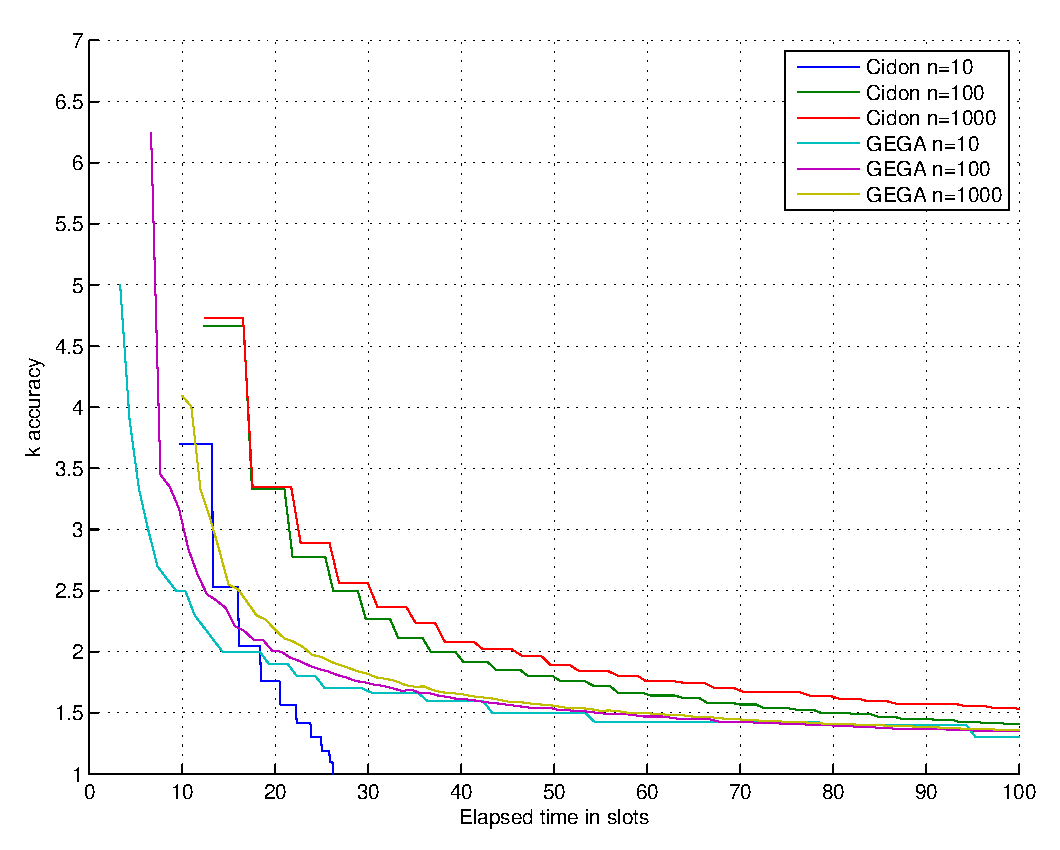
\includegraphics[width=0.8\textwidth]{matlab/Comparison/comparison-gega-cidon}% here 20% wider than \textwidth
 \caption{\emph{GEGA vs Cidon}}
\end{figure}
\end{comment}

In general, we can say that \gega performs great for middle-large batch sizes when we require  $\hat{n}$ to be, with high probability, in the interval $\displaystyle \frac{n}{k}\leq\hat{n}\leq kn$ with $1.5\leq k\leq2$.



\chapter*{Conclusions}
\addcontentsline{toc}{chapter}{Conclusions}
The final goal of this work was to investigate \emph{The Batch Size Estimate Problem} in order to develop, if possible, innovative techniques to solve the problem. Hence, we studied and characterized both the \emph{Batch Size Estimate} and some of the \emph{Batch Resolution Algorithms} to understand in what measure the estimate can influence, and hopefully speedup, the resolution process. There are two possible ways to approach the matter: on one hand you can perform an explicit estimate phase, followed by a resolution one, on the other hand, you can choose to combine the two together. This second option is usually the case in window based scenarios where the result of the resolution is used to preform an estimate and where estimate and resolution processes coincide. Window based approach is really efficient when we have a good knowledge of the batch multiplicity but has the disadvantage that performs really poor when the batch size is different from the expected one. In fact, communication costs are reduced due to deferred feedback but, at the same time, a wrong estimate of the multiplicity results in really poor resolution performance. The big open problem of this approach is how to determine the size of the initial window. A large window results in good estimate and resolution of a possibly large amount of nodes but suffers poor performance if the batch to solve is much smaller than the windows size (empty slots) or much larger (collisions). Using \emph{GEGA} is a great choice in this scenario to determine the batch size in terms of operational range.\\
The main advantages of \emph{GEGA} are:
\begin{itemize}
\item Speed. In fact, for a wide range of minimum required accuracies and batch sizes, it is faster than any other estimate algorithm known to us.
\item Ability to adapt to any batch size. In fact, the time required by the algorithm depends mostly on the user required accuracy and is quite independent of the real batch size  (logarithmic addictive term).
\item Estimate accuracy can be considered independent of the batch size.   
\end{itemize}
However, there are also some limitation to the proposed estimate scheme:
\begin{itemize}
\item It is not able to achieve arbitrary precision in the estimate;
\item When looking for a really tight (almost exact) estimate, other estimate techniques are faster.
\end{itemize}

Therefore we suggest to adopt it to:
\begin{itemize}
\item provide an initial estimate of the batch size which can be further refined using other techniques or that can be used to speedup dynamically estimating resolution processes. 
\item provide an estimate for algorithms that are ``robust'' in terms of resolution efficiency: their performance degrades smoothly when estimated batch size differs, but not too much, from the real one (e.g. \emph{m Groups Splitting}). 
\end{itemize}

Understanding in details how to balance the estimate overhead with the improved resolution efficiency depends on the applied BRA and goes beyond the goals of this work. Just to provide you an idea on how things work, referring, as an example, to the \emph{m Groups Split} in the CSMA scenario described in Section \ref{se:mgroups} we have that, following the notations used throughout this work, if estimate is within the interval $\frac{n}{k}\leq \hat{n}\leq kn$, maximum performance loss is below 3\% when $k=1.5$ and 7\% when $k=2$. Therefore, considering the estimate overhead and choosing the required accuracy in function of the batch size, using GEGA results convenient compared to oblivious resolution (MBT, no estimate performed) when the batch size is larger than 30-70.



\begin{comment}

\begin{sidewaystable}
\centering
\begin{tabular}{|llllllllp{1in}lp{1in}|}
\hline
Context   &Length   &Breadth/   &Depth   &Profile   &Pottery   &Flint   &Animal   &Stone   &Other    &C14 Dates \\
  &         &Diameter   &        &          &          &        & 
Bones&&&\\
\hline
&&&&&&&&&&\\
\multicolumn{10}{|l}{\bf Grooved Ware}&\\
784 &---   &0.90m &0.18m &Sloping U &P1    &$\times$46  &  $\times$8  &&$\times$2 bone&  2150$\pm$ 100 BC\\
785 &---   &1.00m &0.12  &Sloping U &P2--4 &$\times$23  &  $\times$21 & Hammerstone &---&---\\
962 &---   &1.37m &0.20m &Sloping U &P5--6 &$\times$48  &  $\times$57* & ---&     ---&1990 $\pm$ 80 BC (Layer 4) 1870 $\pm$90 BC (Layer 1)\\
983 &0.83m &0.73m &0.25m &Stepped U &---   &$\times$18  &  $\times$8 & ---& Fired clay&---\\
&&&&&&&&&&\\
\multicolumn{10}{|l}{\bf Beaker}&\\
552 &---   &0.68m &0.12m &Saucer    &P7--14 &---        & --- & --- &--- &---\\
790 &---   &0.60m &0.25m &U         &P15    &$\times$12 & --- & Quartzite-lump&--- &---\\
794 &2.89m &0.75m &0.25m &Irreg.    &P16    $\times$3   & --- & --- &--- &---\\
\hline
\end{tabular}
 
\caption[Grooved Ware and Beaker Features, their Finds and Radiocarbon
Dates]{Grooved Ware and Beaker Features, their Finds and Radiocarbon
Dates; For a breakdown of the Pottery Assemblages see Tables I and
III; for the Flints see Tables II and IV; for the Animal Bones see
Table V.}\label{rotfloat2} \end{sidewaystable} 
\end{comment}

\begin{appendices}

\chapter[Appendix]{}

\section{Probability}
\textcolor{red}{sezione provvisoria}
\subsection{Chebyshev's inequality}
Let $X$ be a \emph{random variable} with expected value $\mu$ and finite variance $\sigma^{2}$. Then for any real number $k>0$,
\begin{equation}
\Pr(\left|X-\mu\right|\geq k)\leq\frac{\sigma^{2}}{k^2}
\label{eq:cheby}
\end{equation}
\subsection{Binomial Distribution}

$B(n,p)$
\subsubsection{Poisson Approximation}
The binomial distribution converges towards the Poisson distribution as the number of trials goes to infinity while the product $np$ remains fixed. Therefore the Poisson distribution with parameter $\lambda = np$ can be used as an approximation to $B(n, p)$ of the binomial distribution if $n$ is sufficiently large and $p$ is sufficiently small. According to two rules of thumb, this approximation is good if $n \geq 20$ and $p \leq 0.05$, or if $n \geq 100$ and $np \leq 10$.
\subsubsection{Normal Approximation}
If $n$ is large enough, then the skew of the distribution is not too great. In this case, if a suitable continuity correction is used, then an excellent approximation to $B(n, p)$ is given by the normal distribution $\mathcal{N}(np,np(1-p))$\\
The approximation generally improves as $n$ increases and is better when $p$ is not near to 0 or 1. Various rules of thumb may be used to decide whether $n$ is large enough, and $p$ is far enough from the extremes of zero or unity:
One rule is that both $n p$ and $n(1-p)$ must be greater than 5. However, the specific number varies from source to source, and depends on how good an approximation one wants; some sources give 10.\\

oppure dal libro $np(1-p)\geq 10$.




\subsection{Poisson Distribution}
\subsection{Normal Distribution}
 $\mathcal{N}(\mu,\sigma^{2})$
\begin{equation}
f(x)= \frac{1}{\sqrt{2\pi\sigma^{2}}}\exp{-\frac{(x-\mu)^{2}}{2\sigma^{2}}}
\end{equation}

\section{Greenberg bounded \emph{m}-moments}

In general for base $b$ greenberg algorithm the first and second moments are bounded by:

\begin{equation}
\phi(b)= \frac{1}{\log b} \int_{0}^{\infty} \! e^{-x}(1+x) \prod_{k=1}^{\infty}(1-e^{-b^{k}x}(1+b^{k}x))x^{-2} \, dx
\end{equation}

\begin{equation}
\Phi(b)= \frac{1}{\log b} \int_{0}^{\infty} \! e^{-x}(1+x) \prod_{k=1}^{\infty}(1-e^{-b^{k}x}(1+b^{k}x))x^{-3} \, dx
\end{equation}

\textcolor{red}{note sul calcolo\\ va velocemente a 0 quind basta considerare un intervallo iniziale  limitato\\
anche per produttoria con k è lo stesso.\\ risolto con quad matlab}

\section{CBT Estimate Experimental Distribution}

Following tables \ref{CBT-table-1} shows the behavior of CBT Algorithm (section \ref{cbt-estimation}) for estimation.  Simulation was implemented in matlab.
The resulting distribution of $\hat{n}$ fixed $n$ is the result of averaging \numprint{100000} runs of CBT Algorihm applied on uniformly random generated nodes ID batches.\\ 

\begin{table}[H]
\caption[Experimentally computed CBT Estimate Distributon]{Experimentally computed CBT Estimate Distributon. Table 1/3}
\label{CBT-table-1}
\resizebox{\textwidth}{!}{
\begin{tabular}{r|cccccccccccc}
n&$\hat{n}:$&2&4&8&16&32&64&128&256&512&1024&2048 \\\hline

2 &&0.499 &0.253 &0.125 &0.061 &0.031 &0.015 &0.007 &0.004 &0.002 &9e-04 &4e-04\\\hline

4 &&&0.189 &0.303 &0.225 &0.133 &0.072 &0.038 &0.020 &0.010 &0.005 &0.002\\\hline

8 &&&0.055 &0.212 &0.261 &0.201 &0.126 &0.071 &0.037 &0.019 &0.009 &0.005\\\hline

16 &&&8e-04 &0.070 &0.209 &0.252 &0.197 &0.125 &0.070 &0.038 &0.019 &0.010\\\hline

32 &&&&0.003 &0.075 &0.213 &0.249 &0.195 &0.123 &0.069 &0.037 &0.018\\\hline

64 &&&&&0.004 &0.077 &0.208 &0.250 &0.193 &0.124 &0.069 &0.037\\\hline

128 &&&&&&0.005 &0.081 &0.208 &0.247 &0.191 &0.123 &0.069\\\hline

256 &&&&&&2e-05 &0.006 &0.079 &0.209 &0.246 &0.193 &0.123\\\hline

512 &&&&&&&&0.005 &0.081 &0.207 &0.245 &0.193\\\hline

1024 &&&&&&&&&0.005 &0.080 &0.208 &0.245\\\hline

2048 &&&&&&&&&2e-05 &0.005 &0.080 &0.209\\\hline

4096 &&&&&&&&&&1e-05 &0.006 &0.082\\\hline

8192 &&&&&&&&&&&1e-05 &0.006\\\hline

16384 &&&&&&&&&&&&2e-05\\\hline

32768 &&&&&&&&&&&&\\\hline

\end{tabular}
}

\end{table}
\begin{table}[H]
\ContinuedFloat
\caption[]{Experimentally computed CBT Estimate Distributon. Table 2/3}
\resizebox{\textwidth}{!}{
\begin{tabular}{r|cccccccccccc}
n&$\hat{n}:$&4096&8192&16384&32768&$2^{16}$&$2^{17}$&$2^{18}$&$2^{19}$&$2^{20}$&$2^{21}$&$2^{22}$ \\\hline

2 &&2e-04 &1e-04 &1e-04 &&&&1e-05 &&&&\\\hline

4 &&0.001 &5e-04 &3e-04 &1e-04 &6e-05 &4e-05 &&2e-05 &1e-05 &&\\\hline

8 &&0.002 &0.001 &6e-04 &3e-04 &9e-05 &8e-05 &4e-05 &1e-05 &&&\\\hline

16 &&0.005 &0.003 &0.001 &6e-04 &3e-04 &2e-04 &6e-05 &2e-05 &2e-05 &&\\\hline

32 &&0.009 &0.005 &0.003 &0.001 &6e-04 &3e-04 &1e-04 &1e-04 &6e-05 &1e-05 &1e-05\\\hline

64 &&0.019 &0.009 &0.005 &0.002 &0.001 &7e-04 &3e-04 &7e-05 &4e-05 &&2e-05\\\hline

128 &&0.037 &0.019 &0.010 &0.005 &0.003 &0.001 &5e-04 &4e-04 &2e-04 &5e-05 &4e-05\\\hline

256 &&0.068 &0.038 &0.019 &0.009 &0.005 &0.002 &0.001 &6e-04 &3e-04 &6e-05 &8e-05\\\hline

512 &&0.123 &0.071 &0.037 &0.019 &0.010 &0.005 &0.002 &0.001 &6e-04 &3e-04 &2e-04\\\hline

1024 &&0.193 &0.122 &0.070 &0.037 &0.019 &0.010 &0.005 &0.002 &0.001 &6e-04 &2e-04\\\hline

2048 &&0.246 &0.194 &0.123 &0.068 &0.037 &0.019 &0.010 &0.005 &0.002 &0.001 &6e-04\\\hline

4096 &&0.210 &0.246 &0.193 &0.121 &0.068 &0.037 &0.019 &0.009 &0.004 &0.003 &0.001\\\hline

8192 &&0.080 &0.208 &0.247 &0.192 &0.123 &0.070 &0.037 &0.019 &0.009 &0.005 &0.002\\\hline

16384 &&0.006 &0.080 &0.208 &0.247 &0.192 &0.123 &0.069 &0.037 &0.019 &0.010 &0.005\\\hline

32768 &&&0.006 &0.079 &0.209 &0.248 &0.194 &0.122 &0.069 &0.036 &0.019 &0.010\\\hline

\end{tabular}
}

\end{table}
\begin{table}[H]\ContinuedFloat
\caption[]{Experimentally computed CBT Estimate Distributon. Table 3/3}
\resizebox{\textwidth}{!}{
\begin{tabular}{r|ccccccccccc}
n&$\hat{n}:$&$2^{23}$&$2^{24}$&$2^{25}$&$2^{26}$&$2^{27}$&$2^{28}$&$2^{29}$&$2^{30}$&$2^{31}$&$2^{32}$ \\\hline

2 &&&&&&&&&&&\\\hline

4 &&&&&&&&&&&\\\hline

8 &&&&&&&&&&&\\\hline

16 &&&&&&&&&&&\\\hline

32 &&1e-05 &&&&&&&&&\\\hline

64 &&2e-05 &&&&1e-05 &&&&&\\\hline

128 &&4e-05 &&1e-05 &&&&&&&\\\hline

256 &&4e-05 &1e-05 &&2e-05 &&&1e-05 &&&\\\hline

512 &&7e-05 &2e-05 &1e-05 &3e-05 &1e-05 &&&&&\\\hline

1024 &&2e-04 &1e-04 &4e-05 &&2e-05 &1e-05 &&&&\\\hline

2048 &&3e-04 &1e-04 &3e-05 &3e-05 &3e-05 &3e-05 &&&&\\\hline

4096 &&6e-04 &3e-04 &9e-05 &7e-05 &1e-05 &&&&&\\\hline

8192 &&0.001 &8e-04 &3e-04 &2e-04 &8e-05 &7e-05 &2e-05 &3e-05 &1e-05 &\\\hline

16384 &&0.002 &0.001 &6e-04 &3e-04 &1e-04 &1e-04 &4e-05 &&&\\\hline

32768 &&0.005 &0.002 &0.001 &6e-04 &3e-04 &2e-04 &1e-04 &1e-05 &2e-05 &1e-05\\\hline

\end{tabular}
}
\end{table}

\lstinputlisting{matlab/CBT/cbtsimpletest.m}
\lstinputlisting{matlab/CBT/cbtsplit.m}
\lstinputlisting{matlab/CBT/cbtfulltest.m}
%\verbatiminput{matlab/CBT/cbtfulltest.m}

\section{Greenberg Estimate Distribution}
In following table \ref{basic-greenberg-stop-probabilities} we report how the end  up probability (equation \ref{eq:bgstopprobability}) is distributed among slots given a batch of size $n$.  Column ``$n$'' lists  the considered batch sizes. $\hat{n}$ is the resulting estimation (without corrections) when ending up in the underneath slot.\\  For sake of simplicity considered values are all powers of 2.\\
Datas presented were post-processed to become more accessible:
\begin{itemize}
\item values above $10^{-3}$ are reported in format ('\emph{\%1.3f}');
\item values below $10^{-12}$ are not presented since are tight close to 0.
\item other values are presented in exponential notation and rounded to the first meaningful digit ('\emph{\%1.e}')
\end{itemize}


\begin{sidewaystable}
%%%%%
\flushleft
\resizebox{25cm}{!}{
\begin{tabular}{r|ccccccccccccccccccccccc}
&$\hat{n}$& 2 &4 &8 &16 &32 &64 &128 &256 &512 &1024 &2048 &4096 &8192 &16384 &32768 &65536\\
n & slot:& 1 &2 &3 &4 &5 &6 &7 &8 &9 &10 &11 &12 &13 &14 &15 & 16\\ 
\toprule
1 &&1.000 &&&&&&&&&\\\hline

2 &&0.750 &0.234 &0.015 &2e-04 &1e-06 &9e-10 &&&&&&&&\\\hline

4 &&0.312 &0.508 &0.166 &0.014 &3e-04 &2e-06 &2e-09 &&&&&&&\\\hline

8 &&0.035 &0.354 &0.450 &0.147 &0.013 &3e-04 &2e-06 &4e-09 &1e-12 &&&&&&\\\hline

16 &&3e-04 &0.063 &0.363 &0.422 &0.138 &0.013 &3e-04 &2e-06 &4e-09 &2e-12 &&&&&\\\hline

32 &&8e-09 &0.001 &0.078 &0.366 &0.409 &0.134 &0.013 &3e-04 &2e-06 &4e-09 &2e-12 &&&&\\\hline

64 &&&2e-07 &0.002 &0.084 &0.367 &0.402 &0.131 &0.013 &3e-04 &2e-06 &4e-09 &2e-12 &&&\\\hline

128 &&&&7e-07 &0.002 &0.088 &0.367 &0.399 &0.130 &0.013 &3e-04 &2e-06 &5e-09 &2e-12 &&\\\hline

256 &&&&&1e-06 &0.003 &0.090 &0.368 &0.397 &0.130 &0.013 &3e-04 &2e-06 &5e-09 &2e-12 & \\\hline

512 &&&&&&2e-06 &0.003 &0.090 &0.368 &0.397 &0.130 &0.012 &3e-04 &2e-06 &5e-09 &2e-12 \\\hline
1024 &&&&&&&2e-06 &0.003 &0.091 &0.368 &0.396 &0.129 &0.012 &3e-04 &2e-06 &5e-09 &2e-12 \\
\bottomrule
\end{tabular}
}

\begin{tabular}{c}
\\
\end{tabular}
\resizebox{25cm}{!}{
\begin{tabular}{r|ccccccccccccccccccccccc}
&$\hat{n}$&128 &256 &512 &1024 &2048 &4096 &8192 &16384 &32768 &65536 &$2^{17}$ &$2^{18}$ &$2^{19}$ &$2^{20}$ &$2^{21}$ &$2^{22}$ \\ 
n & slot:& 7 &8 &9 &10 &11 &12 &13 &14 &15 &16 &17 &18 &19 &20 &21 &22 \\ 
\toprule


2048 &&2e-06 &0.003 &0.091 &0.368 &0.396 &0.129 &0.012 &3e-04 &2e-06 &5e-09 &2e-12 &&&&&\\\hline

4096 &&&2e-06 &0.003 &0.091 &0.368 &0.396 &0.129 &0.012 &3e-04 &2e-06 &5e-09 &2e-12 &&&&\\\hline

8192 &&&&2e-06 &0.003 &0.091 &0.368 &0.396 &0.129 &0.012 &3e-04 &2e-06 &5e-09 &2e-12 &&&\\\hline

16384 &&&&&2e-06 &0.003 &0.091 &0.368 &0.396 &0.129 &0.012 &3e-04 &2e-06 &5e-09 &2e-12 &&\\\hline

32768 &&&&&&2e-06 &0.003 &0.091 &0.368 &0.396 &0.129 &0.012 &3e-04 &2e-06 &5e-09 &2e-12 &\\\hline

65536 &&&&&&&2e-06 &0.003 &0.091 &0.368 &0.396 &0.129 &0.012 &3e-04 &2e-06 &5e-09 &2e-12\\

\bottomrule
\end{tabular}
}
%%%%
\caption{Analytically computed basic Greeenberg Estimate Distribution}
\label{basic-greenberg-stop-probabilities}

\end{sidewaystable}

\end{appendices}

\clearpage
\begin{thebibliography}{99}
 
\bibitem{popovski}
  Peter Popovski, Frank H.P. Fitzek, Ramjee Prasad, \emph{ A Class of Algorithms for Collision Resolution with Multiplicity Estimation}, Springer, Algorithmica, Vol. 49, No. 4, December 2007, 286-317
  
\bibitem{lucent}
Murali Kodialam, Thyaga Nandagopal, \emph{Fast and Reliable Estimation Schemes in RFID Systems}, MobiCom '06: Proceedings of the 12th annual international conference on Mobile computing and networking, ACM , September 2006, 322-333 
 
\bibitem{cidon}
 Israel Cidon, Moshe Side, \emph{Conflict Multiplicity Estimation and Batch Resolution Algorithms}, IEEE Transactions On Information Theory, Vol. 34, No. 1, January 1988, 101-110
 
\bibitem{greenberg87}
  Albert G. Greenberg, Philippe Flajolet,  Richard E. Ladner,
  \emph{Estimating the Multiplicities of Conflicts to Speed Their Resolution in Multiple Access Channels},
  Journal of the Association for Computing Machinery,
  Vol 34, No. 2, April 1987, 289-325
  
 \bibitem{capetanakis}
  J.I. Capetanakis, \emph{ Tree algorithms for packet broadcast channels}, IEEE Transactions On Information Theory, Vol. 25, No. 5, September 1979, 505-515
 \end{thebibliography}
\end{document}